% Options for packages loaded elsewhere
% Options for packages loaded elsewhere
\PassOptionsToPackage{unicode}{hyperref}
\PassOptionsToPackage{hyphens}{url}
\PassOptionsToPackage{dvipsnames,svgnames,x11names}{xcolor}
%
\documentclass[
  letterpaper,
  DIV=11,
  numbers=noendperiod]{scrartcl}
\usepackage{xcolor}
\usepackage[top=30mm,left=30mm]{geometry}
\usepackage{amsmath,amssymb}
\setcounter{secnumdepth}{-\maxdimen} % remove section numbering
\usepackage{iftex}
\ifPDFTeX
  \usepackage[T1]{fontenc}
  \usepackage[utf8]{inputenc}
  \usepackage{textcomp} % provide euro and other symbols
\else % if luatex or xetex
  \usepackage{unicode-math} % this also loads fontspec
  \defaultfontfeatures{Scale=MatchLowercase}
  \defaultfontfeatures[\rmfamily]{Ligatures=TeX,Scale=1}
\fi
\usepackage{lmodern}
\ifPDFTeX\else
  % xetex/luatex font selection
\fi
% Use upquote if available, for straight quotes in verbatim environments
\IfFileExists{upquote.sty}{\usepackage{upquote}}{}
\IfFileExists{microtype.sty}{% use microtype if available
  \usepackage[]{microtype}
  \UseMicrotypeSet[protrusion]{basicmath} % disable protrusion for tt fonts
}{}
\makeatletter
\@ifundefined{KOMAClassName}{% if non-KOMA class
  \IfFileExists{parskip.sty}{%
    \usepackage{parskip}
  }{% else
    \setlength{\parindent}{0pt}
    \setlength{\parskip}{6pt plus 2pt minus 1pt}}
}{% if KOMA class
  \KOMAoptions{parskip=half}}
\makeatother
% Make \paragraph and \subparagraph free-standing
\makeatletter
\ifx\paragraph\undefined\else
  \let\oldparagraph\paragraph
  \renewcommand{\paragraph}{
    \@ifstar
      \xxxParagraphStar
      \xxxParagraphNoStar
  }
  \newcommand{\xxxParagraphStar}[1]{\oldparagraph*{#1}\mbox{}}
  \newcommand{\xxxParagraphNoStar}[1]{\oldparagraph{#1}\mbox{}}
\fi
\ifx\subparagraph\undefined\else
  \let\oldsubparagraph\subparagraph
  \renewcommand{\subparagraph}{
    \@ifstar
      \xxxSubParagraphStar
      \xxxSubParagraphNoStar
  }
  \newcommand{\xxxSubParagraphStar}[1]{\oldsubparagraph*{#1}\mbox{}}
  \newcommand{\xxxSubParagraphNoStar}[1]{\oldsubparagraph{#1}\mbox{}}
\fi
\makeatother

\usepackage{color}
\usepackage{fancyvrb}
\newcommand{\VerbBar}{|}
\newcommand{\VERB}{\Verb[commandchars=\\\{\}]}
\DefineVerbatimEnvironment{Highlighting}{Verbatim}{commandchars=\\\{\}}
% Add ',fontsize=\small' for more characters per line
\usepackage{framed}
\definecolor{shadecolor}{RGB}{241,243,245}
\newenvironment{Shaded}{\begin{snugshade}}{\end{snugshade}}
\newcommand{\AlertTok}[1]{\textcolor[rgb]{0.68,0.00,0.00}{#1}}
\newcommand{\AnnotationTok}[1]{\textcolor[rgb]{0.37,0.37,0.37}{#1}}
\newcommand{\AttributeTok}[1]{\textcolor[rgb]{0.40,0.45,0.13}{#1}}
\newcommand{\BaseNTok}[1]{\textcolor[rgb]{0.68,0.00,0.00}{#1}}
\newcommand{\BuiltInTok}[1]{\textcolor[rgb]{0.00,0.23,0.31}{#1}}
\newcommand{\CharTok}[1]{\textcolor[rgb]{0.13,0.47,0.30}{#1}}
\newcommand{\CommentTok}[1]{\textcolor[rgb]{0.37,0.37,0.37}{#1}}
\newcommand{\CommentVarTok}[1]{\textcolor[rgb]{0.37,0.37,0.37}{\textit{#1}}}
\newcommand{\ConstantTok}[1]{\textcolor[rgb]{0.56,0.35,0.01}{#1}}
\newcommand{\ControlFlowTok}[1]{\textcolor[rgb]{0.00,0.23,0.31}{\textbf{#1}}}
\newcommand{\DataTypeTok}[1]{\textcolor[rgb]{0.68,0.00,0.00}{#1}}
\newcommand{\DecValTok}[1]{\textcolor[rgb]{0.68,0.00,0.00}{#1}}
\newcommand{\DocumentationTok}[1]{\textcolor[rgb]{0.37,0.37,0.37}{\textit{#1}}}
\newcommand{\ErrorTok}[1]{\textcolor[rgb]{0.68,0.00,0.00}{#1}}
\newcommand{\ExtensionTok}[1]{\textcolor[rgb]{0.00,0.23,0.31}{#1}}
\newcommand{\FloatTok}[1]{\textcolor[rgb]{0.68,0.00,0.00}{#1}}
\newcommand{\FunctionTok}[1]{\textcolor[rgb]{0.28,0.35,0.67}{#1}}
\newcommand{\ImportTok}[1]{\textcolor[rgb]{0.00,0.46,0.62}{#1}}
\newcommand{\InformationTok}[1]{\textcolor[rgb]{0.37,0.37,0.37}{#1}}
\newcommand{\KeywordTok}[1]{\textcolor[rgb]{0.00,0.23,0.31}{\textbf{#1}}}
\newcommand{\NormalTok}[1]{\textcolor[rgb]{0.00,0.23,0.31}{#1}}
\newcommand{\OperatorTok}[1]{\textcolor[rgb]{0.37,0.37,0.37}{#1}}
\newcommand{\OtherTok}[1]{\textcolor[rgb]{0.00,0.23,0.31}{#1}}
\newcommand{\PreprocessorTok}[1]{\textcolor[rgb]{0.68,0.00,0.00}{#1}}
\newcommand{\RegionMarkerTok}[1]{\textcolor[rgb]{0.00,0.23,0.31}{#1}}
\newcommand{\SpecialCharTok}[1]{\textcolor[rgb]{0.37,0.37,0.37}{#1}}
\newcommand{\SpecialStringTok}[1]{\textcolor[rgb]{0.13,0.47,0.30}{#1}}
\newcommand{\StringTok}[1]{\textcolor[rgb]{0.13,0.47,0.30}{#1}}
\newcommand{\VariableTok}[1]{\textcolor[rgb]{0.07,0.07,0.07}{#1}}
\newcommand{\VerbatimStringTok}[1]{\textcolor[rgb]{0.13,0.47,0.30}{#1}}
\newcommand{\WarningTok}[1]{\textcolor[rgb]{0.37,0.37,0.37}{\textit{#1}}}

\usepackage{longtable,booktabs,array}
\newcounter{none} % for unnumbered tables
\usepackage{calc} % for calculating minipage widths
% Correct order of tables after \paragraph or \subparagraph
\usepackage{etoolbox}
\makeatletter
\patchcmd\longtable{\par}{\if@noskipsec\mbox{}\fi\par}{}{}
\makeatother
% Allow footnotes in longtable head/foot
\IfFileExists{footnotehyper.sty}{\usepackage{footnotehyper}}{\usepackage{footnote}}
\makesavenoteenv{longtable}
\usepackage{graphicx}
\makeatletter
\newsavebox\pandoc@box
\newcommand*\pandocbounded[1]{% scales image to fit in text height/width
  \sbox\pandoc@box{#1}%
  \Gscale@div\@tempa{\textheight}{\dimexpr\ht\pandoc@box+\dp\pandoc@box\relax}%
  \Gscale@div\@tempb{\linewidth}{\wd\pandoc@box}%
  \ifdim\@tempb\p@<\@tempa\p@\let\@tempa\@tempb\fi% select the smaller of both
  \ifdim\@tempa\p@<\p@\scalebox{\@tempa}{\usebox\pandoc@box}%
  \else\usebox{\pandoc@box}%
  \fi%
}
% Set default figure placement to htbp
\def\fps@figure{htbp}
\makeatother





\setlength{\emergencystretch}{3em} % prevent overfull lines

\providecommand{\tightlist}{%
  \setlength{\itemsep}{0pt}\setlength{\parskip}{0pt}}



 


\KOMAoption{captions}{tableheading}
\makeatletter
\@ifpackageloaded{caption}{}{\usepackage{caption}}
\AtBeginDocument{%
\ifdefined\contentsname
  \renewcommand*\contentsname{Table of contents}
\else
  \newcommand\contentsname{Table of contents}
\fi
\ifdefined\listfigurename
  \renewcommand*\listfigurename{List of Figures}
\else
  \newcommand\listfigurename{List of Figures}
\fi
\ifdefined\listtablename
  \renewcommand*\listtablename{List of Tables}
\else
  \newcommand\listtablename{List of Tables}
\fi
\ifdefined\figurename
  \renewcommand*\figurename{Figure}
\else
  \newcommand\figurename{Figure}
\fi
\ifdefined\tablename
  \renewcommand*\tablename{Table}
\else
  \newcommand\tablename{Table}
\fi
}
\@ifpackageloaded{float}{}{\usepackage{float}}
\floatstyle{ruled}
\@ifundefined{c@chapter}{\newfloat{codelisting}{h}{lop}}{\newfloat{codelisting}{h}{lop}[chapter]}
\floatname{codelisting}{Listing}
\newcommand*\listoflistings{\listof{codelisting}{List of Listings}}
\makeatother
\makeatletter
\makeatother
\makeatletter
\@ifpackageloaded{caption}{}{\usepackage{caption}}
\@ifpackageloaded{subcaption}{}{\usepackage{subcaption}}
\makeatother
\usepackage{bookmark}
\IfFileExists{xurl.sty}{\usepackage{xurl}}{} % add URL line breaks if available
\urlstyle{same}
\hypersetup{
  pdftitle={Assessing deepSSF trajectories},
  pdfauthor={Scott Forrest},
  colorlinks=true,
  linkcolor={blue},
  filecolor={Maroon},
  citecolor={Blue},
  urlcolor={Blue},
  pdfcreator={LaTeX via pandoc}}


\title{Assessing deepSSF trajectories}
\author{Scott Forrest}
\date{2025-07-09}
\begin{document}
\maketitle
\begin{abstract}
Now that we have generated trajectories using the
\texttt{deepSSF\_simulations.ipynb} script, we can check how well they
capture different aspects of the observed data. This includes looking at
the distribution of step lengths and turning angles, as well as
comparing the observed and simulated trajectories in terms of the
environmental covariates. We could also further summarise the
trajectories using path-level summaries following a similar approach.
\end{abstract}

\renewcommand*\contentsname{Table of contents}
{
\setcounter{tocdepth}{3}
\tableofcontents
}

\subsection{Loading packages}\label{loading-packages}

\begin{Shaded}
\begin{Highlighting}[]
\FunctionTok{options}\NormalTok{(}\AttributeTok{scipen =} \DecValTok{999}\NormalTok{)}

\FunctionTok{library}\NormalTok{(tidyverse)}
\NormalTok{packages }\OtherTok{\textless{}{-}} \FunctionTok{c}\NormalTok{(}\StringTok{"amt"}\NormalTok{, }\StringTok{"sf"}\NormalTok{, }\StringTok{"terra"}\NormalTok{, }\StringTok{"beepr"}\NormalTok{, }\StringTok{"tictoc"}\NormalTok{, }\StringTok{"viridis"}\NormalTok{, }
              \StringTok{"scales"}\NormalTok{, }\StringTok{"ggpubr"}\NormalTok{, }\StringTok{"zoo"}\NormalTok{)}
\FunctionTok{walk}\NormalTok{(packages, require, }\AttributeTok{character.only =}\NormalTok{ T)}
\end{Highlighting}
\end{Shaded}

\section{Reading in the environmental
covariates}\label{reading-in-the-environmental-covariates}

\begin{Shaded}
\begin{Highlighting}[]
\NormalTok{ndvi }\OtherTok{\textless{}{-}} \FunctionTok{rast}\NormalTok{(}\StringTok{"mapping/cropped rasters/ndvi\_GEE\_projected\_watermask20230207.tif"}\NormalTok{)}
\NormalTok{canopy\_cover }\OtherTok{\textless{}{-}} \FunctionTok{rast}\NormalTok{(}\StringTok{"mapping/cropped rasters/canopy\_cover.tif"}\NormalTok{)}
\NormalTok{veg\_herby }\OtherTok{\textless{}{-}} \FunctionTok{rast}\NormalTok{(}\StringTok{"mapping/cropped rasters/veg\_herby.tif"}\NormalTok{)}
\NormalTok{slope }\OtherTok{\textless{}{-}} \FunctionTok{rast}\NormalTok{(}\StringTok{"mapping/cropped rasters/slope\_raster.tif"}\NormalTok{)}

\CommentTok{\# change the names (these will become the column names when extracting }
\CommentTok{\# covariate values at the used and random steps)}
\FunctionTok{names}\NormalTok{(ndvi) }\OtherTok{\textless{}{-}} \FunctionTok{rep}\NormalTok{(}\StringTok{"ndvi"}\NormalTok{, terra}\SpecialCharTok{::}\FunctionTok{nlyr}\NormalTok{(ndvi))}
\FunctionTok{names}\NormalTok{(canopy\_cover) }\OtherTok{\textless{}{-}} \StringTok{"canopy\_cover"}
\FunctionTok{names}\NormalTok{(veg\_herby) }\OtherTok{\textless{}{-}} \StringTok{"veg\_herby"}
\FunctionTok{names}\NormalTok{(slope) }\OtherTok{\textless{}{-}} \StringTok{"slope"}

\CommentTok{\# for ggplot (and arbitrary index)}
\NormalTok{ndvi\_df }\OtherTok{\textless{}{-}} \FunctionTok{as.data.frame}\NormalTok{(ndvi[[}\DecValTok{1}\NormalTok{]], }\AttributeTok{xy =} \ConstantTok{TRUE}\NormalTok{)}
\CommentTok{\# create discrete breaks for the NDVI for plotting}
\NormalTok{ndvi\_quantiles }\OtherTok{\textless{}{-}} \FunctionTok{quantile}\NormalTok{(ndvi\_df}\SpecialCharTok{$}\NormalTok{ndvi, }\AttributeTok{probs =} \FunctionTok{c}\NormalTok{(}\FloatTok{0.01}\NormalTok{, }\FloatTok{0.99}\NormalTok{))}
\NormalTok{ndvi\_breaks }\OtherTok{\textless{}{-}} \FunctionTok{seq}\NormalTok{(ndvi\_quantiles[}\DecValTok{1}\NormalTok{], ndvi\_quantiles[}\DecValTok{2}\NormalTok{], }\AttributeTok{length.out =} \DecValTok{9}\NormalTok{)}
\NormalTok{ndvi\_df}\SpecialCharTok{$}\NormalTok{ndvi\_discrete }\OtherTok{\textless{}{-}} \FunctionTok{cut}\NormalTok{(ndvi\_df}\SpecialCharTok{$}\NormalTok{ndvi, }\AttributeTok{breaks=}\NormalTok{ndvi\_breaks, }\AttributeTok{dig.lab =} \DecValTok{2}\NormalTok{)}
\end{Highlighting}
\end{Shaded}

\section{Import observed buffalo
data}\label{import-observed-buffalo-data}

\begin{Shaded}
\begin{Highlighting}[]
\NormalTok{buffalo }\OtherTok{\textless{}{-}} \FunctionTok{read\_csv}\NormalTok{(}\StringTok{"data/buffalo\_clean.csv"}\NormalTok{)}
\end{Highlighting}
\end{Shaded}

\begin{verbatim}
Rows: 115776 Columns: 4
-- Column specification --------------------------------------------------------
Delimiter: ","
dbl  (3): x_, y_, id
dttm (1): t_

i Use `spec()` to retrieve the full column specification for this data.
i Specify the column types or set `show_col_types = FALSE` to quiet this message.
\end{verbatim}

\begin{Shaded}
\begin{Highlighting}[]
\FunctionTok{attr}\NormalTok{(buffalo}\SpecialCharTok{$}\NormalTok{t\_, }\StringTok{"tzone"}\NormalTok{) }\OtherTok{\textless{}{-}} \StringTok{"Australia/Queensland"}

\CommentTok{\# plot the data of the buffalo that the deepSSF model was trained with}
\FunctionTok{ggplot}\NormalTok{() }\SpecialCharTok{+}
  \FunctionTok{geom\_point}\NormalTok{(}\AttributeTok{data =}\NormalTok{ buffalo }\SpecialCharTok{|\textgreater{}} \FunctionTok{filter}\NormalTok{(id }\SpecialCharTok{==} \DecValTok{2005}\NormalTok{),}
            \FunctionTok{aes}\NormalTok{(}\AttributeTok{x =}\NormalTok{ x\_, }\AttributeTok{y =}\NormalTok{ y\_, }\AttributeTok{colour =} \FunctionTok{factor}\NormalTok{(id))) }\SpecialCharTok{+}
  \FunctionTok{scale\_colour\_viridis\_d}\NormalTok{() }\SpecialCharTok{+}
  \FunctionTok{coord\_equal}\NormalTok{() }\SpecialCharTok{+}
  \FunctionTok{theme\_bw}\NormalTok{()}
\end{Highlighting}
\end{Shaded}

\pandocbounded{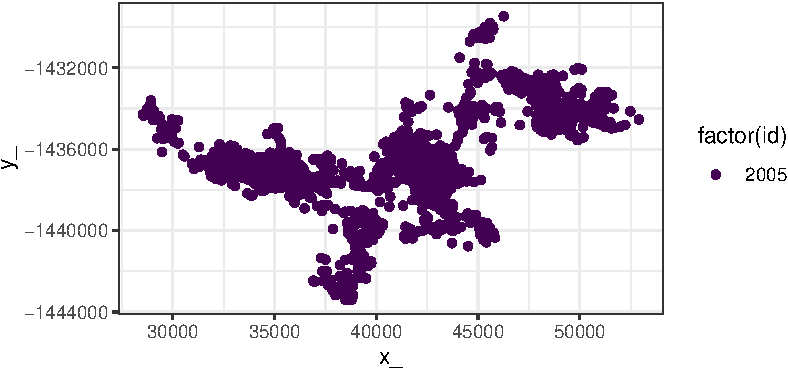
\includegraphics[keepaspectratio]{deepSSF_assessing_trajectories_files/figure-pdf/unnamed-chunk-3-1.pdf}}

\subsection{Calculate step info}\label{calculate-step-info}

\begin{Shaded}
\begin{Highlighting}[]
\NormalTok{hourly\_lag }\OtherTok{\textless{}{-}} \DecValTok{1}

\NormalTok{buffalo }\OtherTok{\textless{}{-}}\NormalTok{ buffalo }\SpecialCharTok{\%\textgreater{}\%} \FunctionTok{mutate}\NormalTok{(}
  \AttributeTok{id =}\NormalTok{ id,}
  \AttributeTok{x1 =}\NormalTok{ x\_,}
  \AttributeTok{y1 =}\NormalTok{ y\_,}
  \AttributeTok{x2 =} \FunctionTok{lead}\NormalTok{(x1, }\AttributeTok{n =}\NormalTok{ hourly\_lag, }\AttributeTok{default =} \ConstantTok{NA}\NormalTok{),}
  \AttributeTok{y2 =} \FunctionTok{lead}\NormalTok{(y1, }\AttributeTok{n =}\NormalTok{ hourly\_lag, }\AttributeTok{default =} \ConstantTok{NA}\NormalTok{),}
  \AttributeTok{t1 =}\NormalTok{ t\_,}
  \AttributeTok{t2 =} \FunctionTok{lead}\NormalTok{(t1, }\AttributeTok{n =}\NormalTok{ hourly\_lag, }\AttributeTok{default =} \ConstantTok{NA}\NormalTok{),}
  \AttributeTok{time\_diff =} \FunctionTok{c}\NormalTok{(}\ConstantTok{NA}\NormalTok{, }\FunctionTok{diff}\NormalTok{(t\_)}\SpecialCharTok{/}\DecValTok{60}\NormalTok{), }\CommentTok{\# time difference in minutes}
  \AttributeTok{hour\_t1 =}\NormalTok{ lubridate}\SpecialCharTok{::}\FunctionTok{hour}\NormalTok{(t\_),}
  \AttributeTok{hour\_t2 =} \FunctionTok{lead}\NormalTok{(hour\_t1, }\AttributeTok{n =}\NormalTok{ hourly\_lag, }\AttributeTok{default =} \ConstantTok{NA}\NormalTok{),}
  \AttributeTok{yday\_t1 =}\NormalTok{ lubridate}\SpecialCharTok{::}\FunctionTok{yday}\NormalTok{(t\_), }\CommentTok{\# day of the year}
  \AttributeTok{yday\_t2 =} \FunctionTok{lead}\NormalTok{(yday\_t1, }\AttributeTok{n =}\NormalTok{ hourly\_lag, }\AttributeTok{default =} \ConstantTok{NA}\NormalTok{),}
  \AttributeTok{sl =} \FunctionTok{c}\NormalTok{(}\FunctionTok{sqrt}\NormalTok{(}\FunctionTok{diff}\NormalTok{(y\_)}\SpecialCharTok{\^{}}\DecValTok{2} \SpecialCharTok{+} \FunctionTok{diff}\NormalTok{(x\_)}\SpecialCharTok{\^{}}\DecValTok{2}\NormalTok{), }\ConstantTok{NA}\NormalTok{), }\CommentTok{\# step lengths}
  \AttributeTok{log\_sl =} \FunctionTok{log}\NormalTok{(sl),}
  \AttributeTok{bearing =} \FunctionTok{c}\NormalTok{(}\FunctionTok{atan2}\NormalTok{(}\FunctionTok{diff}\NormalTok{(y\_), }\FunctionTok{diff}\NormalTok{(x\_)), }\ConstantTok{NA}\NormalTok{),}
  \AttributeTok{ta =} \FunctionTok{c}\NormalTok{(}\ConstantTok{NA}\NormalTok{, }\FunctionTok{ifelse}\NormalTok{(}
    \FunctionTok{diff}\NormalTok{(bearing) }\SpecialCharTok{\textgreater{}}\NormalTok{ pi, }\FunctionTok{diff}\NormalTok{(bearing)}\SpecialCharTok{{-}}\NormalTok{(}\DecValTok{2}\SpecialCharTok{*}\NormalTok{pi), }\FunctionTok{ifelse}\NormalTok{(}
      \FunctionTok{diff}\NormalTok{(bearing) }\SpecialCharTok{\textless{}} \SpecialCharTok{{-}}\NormalTok{pi, }\FunctionTok{diff}\NormalTok{(bearing)}\SpecialCharTok{+}\NormalTok{(}\DecValTok{2}\SpecialCharTok{*}\NormalTok{pi), }\FunctionTok{diff}\NormalTok{(bearing)))), }\CommentTok{\# turning angles}
  \AttributeTok{cos\_ta =} \FunctionTok{cos}\NormalTok{(ta),}
  
  \AttributeTok{.keep =} \StringTok{"none"}
\NormalTok{)}

\FunctionTok{head}\NormalTok{(buffalo)}
\end{Highlighting}
\end{Shaded}

\begin{verbatim}
# A tibble: 6 x 17
     id     x1        y1     x2       y2 t1                  t2                 
  <dbl>  <dbl>     <dbl>  <dbl>    <dbl> <dttm>              <dttm>             
1  2005 41941. -1435875. 41969.  -1.44e6 2018-07-25 10:04:02 2018-07-25 11:04:23
2  2005 41969. -1435671. 41922.  -1.44e6 2018-07-25 11:04:23 2018-07-25 12:04:39
3  2005 41922. -1435654. 41779.  -1.44e6 2018-07-25 12:04:39 2018-07-25 13:04:17
4  2005 41779. -1435601. 41841.  -1.44e6 2018-07-25 13:04:17 2018-07-25 14:04:39
5  2005 41841. -1435635. 41655.  -1.44e6 2018-07-25 14:04:39 2018-07-25 15:04:27
6  2005 41655. -1435604. 41619.  -1.44e6 2018-07-25 15:04:27 2018-07-25 16:04:24
# i 10 more variables: time_diff <dbl>, hour_t1 <int>, hour_t2 <int>,
#   yday_t1 <dbl>, yday_t2 <dbl>, sl <dbl>, log_sl <dbl>, bearing <dbl>,
#   ta <dbl>, cos_ta <dbl>
\end{verbatim}

\subsubsection{To compare the observed buffalo data to the simulated
data, select a subset of the buffalo
data}\label{to-compare-the-observed-buffalo-data-to-the-simulated-data-select-a-subset-of-the-buffalo-data}

\begin{Shaded}
\begin{Highlighting}[]
\NormalTok{no\_subset\_locations }\OtherTok{\textless{}{-}} \DecValTok{3000} \CommentTok{\# to compare to the simulated data}

\NormalTok{buffalo\_id\_subset }\OtherTok{\textless{}{-}}\NormalTok{ buffalo }\CommentTok{\#\%\textgreater{}\% }
  \CommentTok{\# filter(id == 2005) \%\textgreater{}\% }
  \CommentTok{\# arrange(t1) \%\textgreater{}\%  }
  \CommentTok{\# slice(1:no\_subset\_locations)}

\CommentTok{\# hist(buffalo\_id\_subset$time\_diff)}
\end{Highlighting}
\end{Shaded}

\subsection{Import multiple deep learning
trajectories}\label{import-multiple-deep-learning-trajectories}

\begin{Shaded}
\begin{Highlighting}[]
\CommentTok{\# deepSSF model folder}
\NormalTok{deepSSF\_dir }\OtherTok{\textless{}{-}} \StringTok{"id2005\_med\_CNN\_movement\_2\_2025{-}05{-}10"}

\CommentTok{\# read in multiple csv files with similar filenames and bind them together}
\NormalTok{sim\_data\_full\_list }\OtherTok{\textless{}{-}} 
  \FunctionTok{list.files}\NormalTok{(}\FunctionTok{paste0}\NormalTok{(}\StringTok{"Python/outputs/model\_training/"}\NormalTok{,deepSSF\_dir,}\StringTok{"/simulations/deepSSF\_trajectories/"}\NormalTok{), }\AttributeTok{pattern =} \StringTok{"*.csv"}\NormalTok{, }\AttributeTok{full.names =}\NormalTok{ T)[}\DecValTok{1}\SpecialCharTok{:}\DecValTok{50}\NormalTok{]}

\FunctionTok{length}\NormalTok{(sim\_data\_full\_list)}
\end{Highlighting}
\end{Shaded}

\begin{verbatim}
[1] 50
\end{verbatim}

\begin{Shaded}
\begin{Highlighting}[]
\CommentTok{\# to filter filenames with any string matching conditions}
\NormalTok{sim\_data\_filenames }\OtherTok{\textless{}{-}} \FunctionTok{grep}\NormalTok{(}\StringTok{""}\NormalTok{, sim\_data\_full\_list, }\AttributeTok{value =}\NormalTok{ T) }\CommentTok{\#\%\textgreater{}\% }
  \CommentTok{\# grep("3000steps", x = ., value = T) }

\CommentTok{\# read dataframes as a single dataframe with id identifier}
\NormalTok{sim\_data\_all }\OtherTok{\textless{}{-}}\NormalTok{ sim\_data\_filenames }\SpecialCharTok{\%\textgreater{}\%}
  \FunctionTok{map\_dfr}\NormalTok{(read\_csv, }\AttributeTok{.id =} \StringTok{"id"}\NormalTok{) }\SpecialCharTok{\%\textgreater{}\%} 
  \FunctionTok{mutate}\NormalTok{(}
    \AttributeTok{...1 =} \ConstantTok{NULL}
\NormalTok{    )}

\NormalTok{sim\_data\_all}
\end{Highlighting}
\end{Shaded}

\begin{verbatim}
# A tibble: 150,000 x 6
   id         x         y  hour  yday bearing
   <chr>  <dbl>     <dbl> <dbl> <dbl>   <dbl>
 1 1     41969. -1435671      0   206  -2.86 
 2 1     41856. -1435879.     1   206  -2.07 
 3 1     42373. -1436237.     2   206  -0.605
 4 1     42356. -1436233.     3   206   2.95 
 5 1     42357. -1436241.     4   206  -1.43 
 6 1     42367. -1436234.     5   206   0.593
 7 1     42366. -1436245.     6   206  -1.74 
 8 1     42462. -1436232.     7   206   0.130
 9 1     42464. -1436242.     8   206  -1.34 
10 1     42291. -1436407.     9   206  -2.38 
# i 149,990 more rows
\end{verbatim}

\subsection{Calculate step lengths and turning angles
etc}\label{calculate-step-lengths-and-turning-angles-etc}

\begin{Shaded}
\begin{Highlighting}[]
\NormalTok{hourly\_lag }\OtherTok{\textless{}{-}} \DecValTok{1}

\CommentTok{\# Nest the data by \textquotesingle{}id\textquotesingle{}}
\NormalTok{sim\_data\_nested }\OtherTok{\textless{}{-}}\NormalTok{ sim\_data\_all }\SpecialCharTok{\%\textgreater{}\%} 
  \FunctionTok{group\_by}\NormalTok{(id) }\SpecialCharTok{\%\textgreater{}\%}
  \FunctionTok{nest}\NormalTok{()}

\CommentTok{\# Map the mutate transformation over each nested tibble}
\NormalTok{sim\_data\_nested }\OtherTok{\textless{}{-}}\NormalTok{ sim\_data\_nested }\SpecialCharTok{\%\textgreater{}\%}
  \FunctionTok{mutate}\NormalTok{(}\AttributeTok{data =} \FunctionTok{map}\NormalTok{(data, }\SpecialCharTok{\textasciitilde{}}\NormalTok{ .x }\SpecialCharTok{\%\textgreater{}\%}
    \FunctionTok{mutate}\NormalTok{(}
      \AttributeTok{x1 =}\NormalTok{ x,}
      \AttributeTok{y1 =}\NormalTok{ y,}
      \AttributeTok{x2 =} \FunctionTok{lead}\NormalTok{(x1, }\AttributeTok{n =}\NormalTok{ hourly\_lag, }\AttributeTok{default =} \ConstantTok{NA}\NormalTok{),}
      \AttributeTok{y2 =} \FunctionTok{lead}\NormalTok{(y1, }\AttributeTok{n =}\NormalTok{ hourly\_lag, }\AttributeTok{default =} \ConstantTok{NA}\NormalTok{),}
      \AttributeTok{date =} \FunctionTok{as.Date}\NormalTok{(yday }\SpecialCharTok{{-}} \DecValTok{1}\NormalTok{, }\AttributeTok{origin =} \StringTok{"2018{-}01{-}01"}\NormalTok{),}
      \AttributeTok{t1 =} \FunctionTok{as.POSIXct}\NormalTok{(}\FunctionTok{paste}\NormalTok{(date, hour), }\AttributeTok{format =} \StringTok{"\%Y{-}\%m{-}\%d \%H"}\NormalTok{),}
      \AttributeTok{t2 =} \FunctionTok{lead}\NormalTok{(t1, }\AttributeTok{n =}\NormalTok{ hourly\_lag, }\AttributeTok{default =} \ConstantTok{NA}\NormalTok{),}
      \AttributeTok{yday\_t1 =}\NormalTok{ lubridate}\SpecialCharTok{::}\FunctionTok{yday}\NormalTok{(t1), }\CommentTok{\# day of the year}
      \AttributeTok{yday\_t2 =} \FunctionTok{lead}\NormalTok{(yday\_t1, }\AttributeTok{n =}\NormalTok{ hourly\_lag, }\AttributeTok{default =} \ConstantTok{NA}\NormalTok{),}
      \AttributeTok{hour\_t1 =}\NormalTok{ lubridate}\SpecialCharTok{::}\FunctionTok{hour}\NormalTok{(t1),}
      \AttributeTok{hour\_t2 =} \FunctionTok{lead}\NormalTok{(hour\_t1, }\AttributeTok{n =}\NormalTok{ hourly\_lag, }\AttributeTok{default =} \ConstantTok{NA}\NormalTok{),}
      \AttributeTok{sl =} \FunctionTok{c}\NormalTok{(}\FunctionTok{sqrt}\NormalTok{(}\FunctionTok{diff}\NormalTok{(y)}\SpecialCharTok{\^{}}\DecValTok{2} \SpecialCharTok{+} \FunctionTok{diff}\NormalTok{(x)}\SpecialCharTok{\^{}}\DecValTok{2}\NormalTok{), }\ConstantTok{NA}\NormalTok{),  }\CommentTok{\# step lengths}
      \AttributeTok{log\_sl =} \FunctionTok{log}\NormalTok{(sl),}
      \AttributeTok{bearing =} \FunctionTok{c}\NormalTok{(}\FunctionTok{atan2}\NormalTok{(}\FunctionTok{diff}\NormalTok{(y), }\FunctionTok{diff}\NormalTok{(x)), }\ConstantTok{NA}\NormalTok{),}
      \AttributeTok{ta =} \FunctionTok{c}\NormalTok{(}\ConstantTok{NA}\NormalTok{, }\FunctionTok{ifelse}\NormalTok{(}
        \FunctionTok{diff}\NormalTok{(bearing) }\SpecialCharTok{\textgreater{}}\NormalTok{ pi, }\FunctionTok{diff}\NormalTok{(bearing) }\SpecialCharTok{{-}}\NormalTok{ (}\DecValTok{2} \SpecialCharTok{*}\NormalTok{ pi),}
        \FunctionTok{ifelse}\NormalTok{(}\FunctionTok{diff}\NormalTok{(bearing) }\SpecialCharTok{\textless{}} \SpecialCharTok{{-}}\NormalTok{pi, }\FunctionTok{diff}\NormalTok{(bearing) }\SpecialCharTok{+}\NormalTok{ (}\DecValTok{2} \SpecialCharTok{*}\NormalTok{ pi), }\FunctionTok{diff}\NormalTok{(bearing))}
\NormalTok{      )),}
      \AttributeTok{cos\_ta =} \FunctionTok{cos}\NormalTok{(ta),}
      
      \AttributeTok{.keep =} \StringTok{"none"}
\NormalTok{    )}
\NormalTok{  ))}

\CommentTok{\# Unnest the transformed data back into a single data frame}
\NormalTok{sim\_data\_all }\OtherTok{\textless{}{-}}\NormalTok{ sim\_data\_nested }\SpecialCharTok{\%\textgreater{}\%} 
  \FunctionTok{unnest}\NormalTok{(data) }\SpecialCharTok{\%\textgreater{}\%} 
  \FunctionTok{ungroup}\NormalTok{() }\SpecialCharTok{\%\textgreater{}\%} 
  \FunctionTok{mutate}\NormalTok{(}\AttributeTok{id =} \FunctionTok{as.numeric}\NormalTok{(id))}

\FunctionTok{head}\NormalTok{(sim\_data\_all)}
\end{Highlighting}
\end{Shaded}

\begin{verbatim}
# A tibble: 6 x 17
     id bearing     x1        y1     x2        y2 date       t1                 
  <dbl>   <dbl>  <dbl>     <dbl>  <dbl>     <dbl> <date>     <dttm>             
1     1  -2.07  41969. -1435671  41856. -1435879. 2018-07-25 2018-07-25 00:00:00
2     1  -0.605 41856. -1435879. 42373. -1436237. 2018-07-25 2018-07-25 01:00:00
3     1   2.95  42373. -1436237. 42356. -1436233. 2018-07-25 2018-07-25 02:00:00
4     1  -1.43  42356. -1436233. 42357. -1436241. 2018-07-25 2018-07-25 03:00:00
5     1   0.593 42357. -1436241. 42367. -1436234. 2018-07-25 2018-07-25 04:00:00
6     1  -1.74  42367. -1436234. 42366. -1436245. 2018-07-25 2018-07-25 05:00:00
# i 9 more variables: t2 <dttm>, yday_t1 <dbl>, yday_t2 <dbl>, hour_t1 <int>,
#   hour_t2 <int>, sl <dbl>, log_sl <dbl>, ta <dbl>, cos_ta <dbl>
\end{verbatim}

\subsection{Combine the observed and simulated
datasets}\label{combine-the-observed-and-simulated-datasets}

\begin{Shaded}
\begin{Highlighting}[]
\NormalTok{all\_data }\OtherTok{\textless{}{-}} \FunctionTok{bind\_rows}\NormalTok{(buffalo\_id\_subset, sim\_data\_all)}
\FunctionTok{head}\NormalTok{(all\_data)}
\end{Highlighting}
\end{Shaded}

\begin{verbatim}
# A tibble: 6 x 18
     id     x1        y1     x2       y2 t1                  t2                 
  <dbl>  <dbl>     <dbl>  <dbl>    <dbl> <dttm>              <dttm>             
1  2005 41941. -1435875. 41969.  -1.44e6 2018-07-25 10:04:02 2018-07-25 11:04:23
2  2005 41969. -1435671. 41922.  -1.44e6 2018-07-25 11:04:23 2018-07-25 12:04:39
3  2005 41922. -1435654. 41779.  -1.44e6 2018-07-25 12:04:39 2018-07-25 13:04:17
4  2005 41779. -1435601. 41841.  -1.44e6 2018-07-25 13:04:17 2018-07-25 14:04:39
5  2005 41841. -1435635. 41655.  -1.44e6 2018-07-25 14:04:39 2018-07-25 15:04:27
6  2005 41655. -1435604. 41619.  -1.44e6 2018-07-25 15:04:27 2018-07-25 16:04:24
# i 11 more variables: time_diff <dbl>, hour_t1 <int>, hour_t2 <int>,
#   yday_t1 <dbl>, yday_t2 <dbl>, sl <dbl>, log_sl <dbl>, bearing <dbl>,
#   ta <dbl>, cos_ta <dbl>, date <date>
\end{verbatim}

\subsubsection{Prepare trajectories for
plotting}\label{prepare-trajectories-for-plotting}

\begin{Shaded}
\begin{Highlighting}[]
\CommentTok{\# set a buffer around the minimum and maximum x and y values}
\NormalTok{buffer }\OtherTok{\textless{}{-}} \DecValTok{2500}

\CommentTok{\# set the extent of the plot}
\NormalTok{plot\_extent }\OtherTok{\textless{}{-}}\NormalTok{ all\_data }\SpecialCharTok{\%\textgreater{}\%} \FunctionTok{filter}\NormalTok{(id }\SpecialCharTok{\%in\%} \DecValTok{1}\SpecialCharTok{:}\DecValTok{5}\NormalTok{) }\SpecialCharTok{\%\textgreater{}\%} 
  \FunctionTok{summarise}\NormalTok{(}\AttributeTok{min\_x =} \FunctionTok{min}\NormalTok{(x1) }\SpecialCharTok{{-}} \DecValTok{2500}\NormalTok{, }\AttributeTok{min\_y =} \FunctionTok{min}\NormalTok{(y1) }\SpecialCharTok{{-}} \DecValTok{2500}\NormalTok{, }\AttributeTok{max\_x =} \FunctionTok{max}\NormalTok{(x1) }\SpecialCharTok{+} \DecValTok{2500}\NormalTok{, }\AttributeTok{max\_y =} \FunctionTok{max}\NormalTok{(y1) }\SpecialCharTok{+} \DecValTok{2500}\NormalTok{)}

\CommentTok{\# Remove cells outside the extent of the simulated locations (with the buffer)}
\NormalTok{ndvi\_df }\OtherTok{\textless{}{-}}\NormalTok{ ndvi\_df }\SpecialCharTok{\%\textgreater{}\%}
  \FunctionTok{filter}\NormalTok{(x }\SpecialCharTok{\textgreater{}=}\NormalTok{ plot\_extent[[}\DecValTok{1}\NormalTok{]] }\SpecialCharTok{\&}\NormalTok{ x }\SpecialCharTok{\textless{}=}\NormalTok{ plot\_extent[[}\DecValTok{3}\NormalTok{]] }\SpecialCharTok{\&} 
\NormalTok{           y }\SpecialCharTok{\textgreater{}=}\NormalTok{ plot\_extent[[}\DecValTok{2}\NormalTok{]] }\SpecialCharTok{\&}\NormalTok{ y }\SpecialCharTok{\textless{}=}\NormalTok{ plot\_extent[[}\DecValTok{4}\NormalTok{]]) }\SpecialCharTok{\%\textgreater{}\%} 
  \FunctionTok{mutate}\NormalTok{(}
    \AttributeTok{x\_scaled =}\NormalTok{ (x }\SpecialCharTok{{-}}\NormalTok{ plot\_extent[[}\DecValTok{1}\NormalTok{]])}\SpecialCharTok{/}\DecValTok{1000}\NormalTok{,}
    \AttributeTok{y\_scaled =}\NormalTok{ (y }\SpecialCharTok{{-}}\NormalTok{ plot\_extent[[}\DecValTok{2}\NormalTok{]])}\SpecialCharTok{/}\DecValTok{1000}
\NormalTok{  )}

\CommentTok{\# Scale the x and y coordinates of the observed and simulated data}
\NormalTok{all\_data }\OtherTok{\textless{}{-}}\NormalTok{ all\_data }\SpecialCharTok{\%\textgreater{}\%}
  \FunctionTok{mutate}\NormalTok{(}
    \AttributeTok{x1\_scaled =}\NormalTok{ (x1 }\SpecialCharTok{{-}}\NormalTok{ plot\_extent[[}\DecValTok{1}\NormalTok{]])}\SpecialCharTok{/}\DecValTok{1000}\NormalTok{,}
    \AttributeTok{y1\_scaled =}\NormalTok{ (y1 }\SpecialCharTok{{-}}\NormalTok{ plot\_extent[[}\DecValTok{2}\NormalTok{]])}\SpecialCharTok{/}\DecValTok{1000}
\NormalTok{  )}
\end{Highlighting}
\end{Shaded}

\subsection{Plot the obsereved and simulated
trajectories}\label{plot-the-obsereved-and-simulated-trajectories}

\begin{Shaded}
\begin{Highlighting}[]
\FunctionTok{ggplot}\NormalTok{() }\SpecialCharTok{+}
  
  \FunctionTok{geom\_raster}\NormalTok{(}\AttributeTok{data =}\NormalTok{ ndvi\_df, }
                      \FunctionTok{aes}\NormalTok{(}\AttributeTok{x =}\NormalTok{ x\_scaled, }\AttributeTok{y =}\NormalTok{ y\_scaled, }\AttributeTok{fill =}\NormalTok{ ndvi\_discrete), }
                      \AttributeTok{alpha =} \FloatTok{0.75}\NormalTok{) }\SpecialCharTok{+}
  \FunctionTok{scale\_fill\_brewer}\NormalTok{(}\StringTok{"ndvi"}\NormalTok{, }\AttributeTok{palette =} \StringTok{"Greys"}\NormalTok{, }
                    \AttributeTok{guide =} \FunctionTok{guide\_legend}\NormalTok{(}\AttributeTok{reverse =} \ConstantTok{TRUE}\NormalTok{)) }\SpecialCharTok{+}
  
  \FunctionTok{geom\_path}\NormalTok{(}\AttributeTok{data =}\NormalTok{ all\_data }\SpecialCharTok{\%\textgreater{}\%} \FunctionTok{filter}\NormalTok{(id }\SpecialCharTok{\%in\%} \DecValTok{1}\SpecialCharTok{:}\DecValTok{5}\NormalTok{),}
            \FunctionTok{aes}\NormalTok{(}\AttributeTok{x =}\NormalTok{ x1\_scaled, }\AttributeTok{y =}\NormalTok{ y1\_scaled, }\AttributeTok{colour =} \FunctionTok{as.factor}\NormalTok{(id)), }
            \AttributeTok{alpha =} \FloatTok{0.75}\NormalTok{, }\AttributeTok{linewidth =} \FloatTok{0.25}\NormalTok{) }\SpecialCharTok{+}
  
  \FunctionTok{scale\_colour\_viridis\_d}\NormalTok{() }\SpecialCharTok{+}
  
  \FunctionTok{geom\_path}\NormalTok{(}\AttributeTok{data =}\NormalTok{ all\_data }\SpecialCharTok{\%\textgreater{}\%} \FunctionTok{filter}\NormalTok{(id }\SpecialCharTok{==} \DecValTok{2005}\NormalTok{),}
            \FunctionTok{aes}\NormalTok{(}\AttributeTok{x =}\NormalTok{ x1\_scaled, }\AttributeTok{y =}\NormalTok{ y1\_scaled), }
            \AttributeTok{alpha =} \FloatTok{0.75}\NormalTok{, }\AttributeTok{linewidth =} \FloatTok{0.25}\NormalTok{, }\AttributeTok{colour =} \StringTok{"red"}\NormalTok{) }\SpecialCharTok{+}
  
  \FunctionTok{geom\_point}\NormalTok{(}\AttributeTok{data =}\NormalTok{ all\_data }\SpecialCharTok{\%\textgreater{}\%} \FunctionTok{slice}\NormalTok{(}\DecValTok{1}\NormalTok{),}
            \FunctionTok{aes}\NormalTok{(}\AttributeTok{x =}\NormalTok{ x1\_scaled, }\AttributeTok{y =}\NormalTok{ y1\_scaled), }\AttributeTok{fill =} \StringTok{"blue"}\NormalTok{, }\AttributeTok{shape =} \DecValTok{23}\NormalTok{) }\SpecialCharTok{+}
  
  \FunctionTok{scale\_x\_continuous}\NormalTok{(}\StringTok{"Easting (km)"}\NormalTok{,}
                     \AttributeTok{expand =} \FunctionTok{c}\NormalTok{(}\DecValTok{0}\NormalTok{, }\DecValTok{0}\NormalTok{)) }\SpecialCharTok{+}
  \FunctionTok{scale\_y\_continuous}\NormalTok{(}\StringTok{"Northing (km)"}\NormalTok{,}
                     \AttributeTok{expand =} \FunctionTok{c}\NormalTok{(}\DecValTok{0}\NormalTok{, }\DecValTok{0}\NormalTok{)) }\SpecialCharTok{+}
  \FunctionTok{coord\_equal}\NormalTok{() }\SpecialCharTok{+}
  \FunctionTok{theme\_bw}\NormalTok{() }\SpecialCharTok{+}
  \FunctionTok{theme}\NormalTok{(}\AttributeTok{legend.position =} \StringTok{"none"}\NormalTok{)}
\end{Highlighting}
\end{Shaded}

\begin{verbatim}
Warning: Removed 70627 rows containing missing values or values outside the scale range
(`geom_raster()`).
\end{verbatim}

\pandocbounded{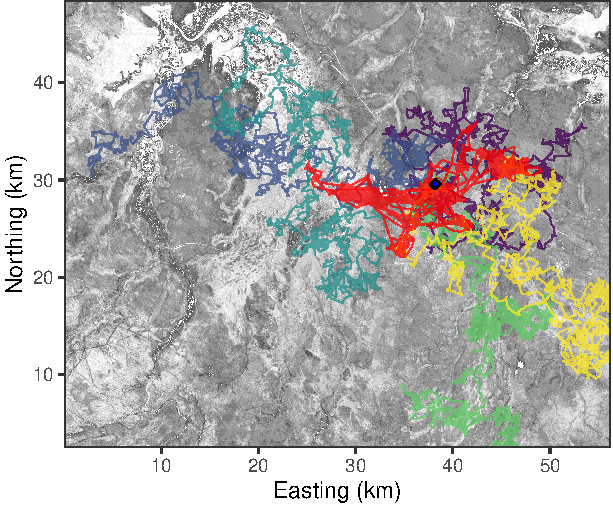
\includegraphics[keepaspectratio]{deepSSF_assessing_trajectories_files/figure-pdf/unnamed-chunk-10-1.pdf}}

\begin{Shaded}
\begin{Highlighting}[]
\FunctionTok{ggsave}\NormalTok{(}\FunctionTok{paste0}\NormalTok{(}\StringTok{"Python/outputs/model\_training/"}\NormalTok{,deepSSF\_dir,}\StringTok{"/simulated\_trajectories.png"}\NormalTok{), }\AttributeTok{width=}\DecValTok{150}\NormalTok{, }\AttributeTok{height=}\DecValTok{150}\NormalTok{, }\AttributeTok{units=}\StringTok{"mm"}\NormalTok{, }\AttributeTok{dpi =} \DecValTok{600}\NormalTok{)}
\end{Highlighting}
\end{Shaded}

\begin{verbatim}
Warning: Removed 70627 rows containing missing values or values outside the scale range
(`geom_raster()`).
\end{verbatim}

\section{Plot movement distributions}\label{plot-movement-distributions}

The skyblue density plot represents the observed data and the orange
density plot represents the simulated data.

\subsection{Step lengths}\label{step-lengths}

\begin{Shaded}
\begin{Highlighting}[]
\NormalTok{cell\_widths }\OtherTok{\textless{}{-}} \FunctionTok{data.frame}\NormalTok{(}\AttributeTok{x =} \FunctionTok{c}\NormalTok{(}\DecValTok{0}\NormalTok{, }\FloatTok{12.5}\NormalTok{, }\FunctionTok{seq}\NormalTok{(}\FloatTok{37.5}\NormalTok{, }\DecValTok{1785}\NormalTok{, }\AttributeTok{by =} \DecValTok{25}\NormalTok{)), }\AttributeTok{y =} \DecValTok{0}\NormalTok{)}

\NormalTok{step\_lengths\_stationary }\OtherTok{\textless{}{-}} \FunctionTok{ggplot}\NormalTok{() }\SpecialCharTok{+}
  \CommentTok{\# geom\_vline(data = cell\_widths,}
  \CommentTok{\#            aes(xintercept = x), }
  \CommentTok{\#            colour = "black", linetype = "dashed", alpha = 0.5) +}
  \FunctionTok{geom\_density}\NormalTok{(}\AttributeTok{data =}\NormalTok{ all\_data }\SpecialCharTok{\%\textgreater{}\%} \FunctionTok{filter}\NormalTok{(id }\SpecialCharTok{==} \DecValTok{2005}\NormalTok{),}
                 \FunctionTok{aes}\NormalTok{(}\AttributeTok{x =}\NormalTok{ sl),}
                 \AttributeTok{fill =} \StringTok{"skyblue"}\NormalTok{, }\AttributeTok{colour =} \StringTok{"skyblue"}\NormalTok{, }\AttributeTok{alpha =} \FloatTok{0.5}\NormalTok{) }\SpecialCharTok{+}
  \FunctionTok{geom\_density}\NormalTok{(}\AttributeTok{data =}\NormalTok{ all\_data }\SpecialCharTok{\%\textgreater{}\%} \FunctionTok{filter}\NormalTok{(}\SpecialCharTok{!}\NormalTok{id }\SpecialCharTok{==} \DecValTok{2005}\NormalTok{),}
                 \FunctionTok{aes}\NormalTok{(}\AttributeTok{x =}\NormalTok{ sl),}
                 \AttributeTok{fill =} \StringTok{"orange"}\NormalTok{, }\AttributeTok{colour =} \StringTok{"orange"}\NormalTok{, }\AttributeTok{alpha =} \FloatTok{0.5}\NormalTok{) }\SpecialCharTok{+}
  \FunctionTok{scale\_x\_continuous}\NormalTok{(}\StringTok{"Step length (m)"}\NormalTok{, }\AttributeTok{limits =} \FunctionTok{c}\NormalTok{(}\DecValTok{0}\NormalTok{, }\DecValTok{1500}\NormalTok{)) }\SpecialCharTok{+}
  \FunctionTok{scale\_y\_continuous}\NormalTok{(}\StringTok{"Density"}\NormalTok{) }\SpecialCharTok{+}
  \FunctionTok{theme\_bw}\NormalTok{()}

\NormalTok{step\_lengths\_stationary}
\end{Highlighting}
\end{Shaded}

\begin{verbatim}
Warning: Removed 147 rows containing non-finite outside the scale range
(`stat_density()`).
\end{verbatim}

\begin{verbatim}
Warning: Removed 3703 rows containing non-finite outside the scale range
(`stat_density()`).
\end{verbatim}

\pandocbounded{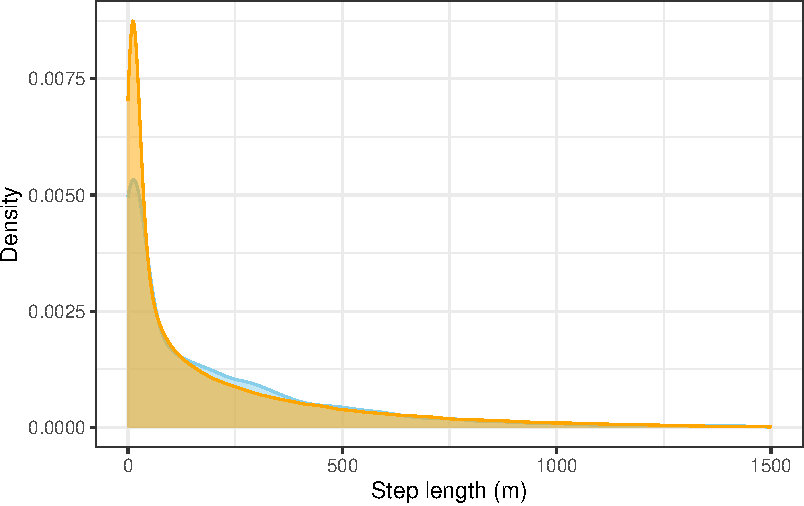
\includegraphics[keepaspectratio]{deepSSF_assessing_trajectories_files/figure-pdf/unnamed-chunk-11-1.pdf}}

\begin{Shaded}
\begin{Highlighting}[]
\FunctionTok{ggsave}\NormalTok{(}\FunctionTok{paste0}\NormalTok{(}\StringTok{"Python/outputs/model\_training/"}\NormalTok{,deepSSF\_dir,}\StringTok{"/step\_lengths.png"}\NormalTok{), }\AttributeTok{width=}\DecValTok{150}\NormalTok{, }\AttributeTok{height=}\DecValTok{80}\NormalTok{, }\AttributeTok{units=}\StringTok{"mm"}\NormalTok{, }\AttributeTok{dpi =} \DecValTok{600}\NormalTok{)}
\end{Highlighting}
\end{Shaded}

\begin{verbatim}
Warning: Removed 147 rows containing non-finite outside the scale range
(`stat_density()`).
Removed 3703 rows containing non-finite outside the scale range
(`stat_density()`).
\end{verbatim}

\subsection{Log step lengths}\label{log-step-lengths}

\begin{Shaded}
\begin{Highlighting}[]
\NormalTok{step\_lengths\_log }\OtherTok{\textless{}{-}} \FunctionTok{ggplot}\NormalTok{() }\SpecialCharTok{+}
  \FunctionTok{geom\_vline}\NormalTok{(}\AttributeTok{data =}\NormalTok{ cell\_widths,}
             \FunctionTok{aes}\NormalTok{(}\AttributeTok{xintercept =}\NormalTok{ x), }
             \AttributeTok{colour =} \StringTok{"black"}\NormalTok{, }\AttributeTok{linetype =} \StringTok{"dashed"}\NormalTok{, }\AttributeTok{alpha =} \FloatTok{0.5}\NormalTok{) }\SpecialCharTok{+}
  \FunctionTok{geom\_density}\NormalTok{(}\AttributeTok{data =}\NormalTok{ all\_data }\SpecialCharTok{\%\textgreater{}\%} \FunctionTok{filter}\NormalTok{(id }\SpecialCharTok{==} \DecValTok{2005}\NormalTok{),}
                 \FunctionTok{aes}\NormalTok{(}\AttributeTok{x =}\NormalTok{ sl),}
                 \AttributeTok{fill =} \StringTok{"skyblue"}\NormalTok{, }\AttributeTok{colour =} \StringTok{"skyblue"}\NormalTok{, }\AttributeTok{alpha =} \FloatTok{0.5}\NormalTok{) }\SpecialCharTok{+}
  \FunctionTok{geom\_density}\NormalTok{(}\AttributeTok{data =}\NormalTok{ all\_data }\SpecialCharTok{\%\textgreater{}\%} \FunctionTok{filter}\NormalTok{(}\SpecialCharTok{!}\NormalTok{id }\SpecialCharTok{==} \DecValTok{2005}\NormalTok{),}
                 \FunctionTok{aes}\NormalTok{(}\AttributeTok{x =}\NormalTok{ sl),}
                 \AttributeTok{fill =} \StringTok{"orange"}\NormalTok{, }\AttributeTok{colour =} \StringTok{"orange"}\NormalTok{, }\AttributeTok{alpha =} \FloatTok{0.5}\NormalTok{) }\SpecialCharTok{+}
  \FunctionTok{scale\_x\_log10}\NormalTok{(}\StringTok{"log Step length (m)"}\NormalTok{) }\SpecialCharTok{+}
  \FunctionTok{scale\_y\_continuous}\NormalTok{(}\StringTok{"Density"}\NormalTok{) }\SpecialCharTok{+}
  \FunctionTok{theme\_bw}\NormalTok{()}

\NormalTok{step\_lengths\_log}
\end{Highlighting}
\end{Shaded}

\begin{verbatim}
Warning in scale_x_log10("log Step length (m)"): log-10 transformation
introduced infinite values.
\end{verbatim}

\begin{verbatim}
Warning: Removed 51 rows containing non-finite outside the scale range
(`stat_density()`).
\end{verbatim}

\pandocbounded{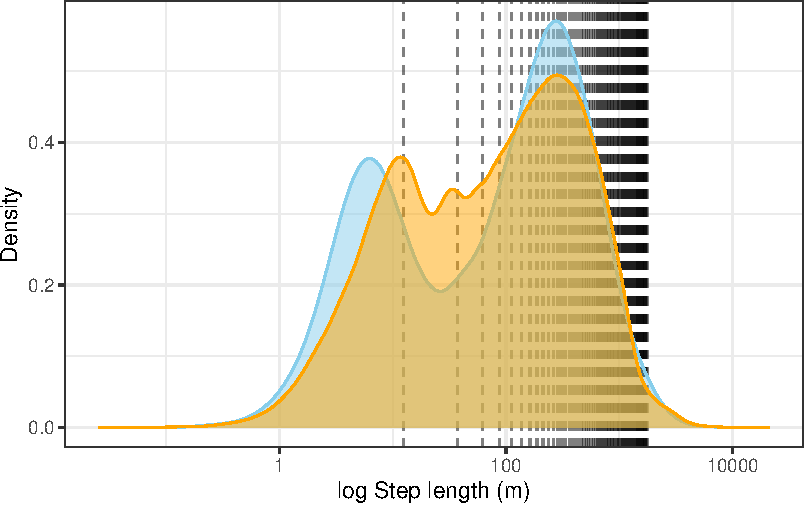
\includegraphics[keepaspectratio]{deepSSF_assessing_trajectories_files/figure-pdf/unnamed-chunk-12-1.pdf}}

\begin{Shaded}
\begin{Highlighting}[]
\FunctionTok{ggsave}\NormalTok{(}\FunctionTok{paste0}\NormalTok{(}\StringTok{"Python/outputs/model\_training/"}\NormalTok{,deepSSF\_dir,}\StringTok{"/log\_sl.png"}\NormalTok{), }\AttributeTok{width=}\DecValTok{150}\NormalTok{, }\AttributeTok{height=}\DecValTok{80}\NormalTok{, }\AttributeTok{units=}\StringTok{"mm"}\NormalTok{, }\AttributeTok{dpi =} \DecValTok{600}\NormalTok{)}
\end{Highlighting}
\end{Shaded}

\begin{verbatim}
Warning in scale_x_log10("log Step length (m)"): log-10 transformation introduced infinite values.
Removed 51 rows containing non-finite outside the scale range
(`stat_density()`).
\end{verbatim}

\subsection{Turning angles}\label{turning-angles}

\begin{Shaded}
\begin{Highlighting}[]
\NormalTok{turning\_angles\_stationary }\OtherTok{\textless{}{-}} \FunctionTok{ggplot}\NormalTok{() }\SpecialCharTok{+}
  \FunctionTok{geom\_density}\NormalTok{(}\AttributeTok{data =}\NormalTok{ all\_data }\SpecialCharTok{\%\textgreater{}\%} \FunctionTok{filter}\NormalTok{(id }\SpecialCharTok{==} \DecValTok{2005}\NormalTok{),}
                 \FunctionTok{aes}\NormalTok{(}\AttributeTok{x =}\NormalTok{ ta),}
                 \AttributeTok{fill =} \StringTok{"skyblue"}\NormalTok{, }\AttributeTok{colour =} \StringTok{"skyblue"}\NormalTok{, }\AttributeTok{alpha =} \FloatTok{0.5}\NormalTok{) }\SpecialCharTok{+}
  \FunctionTok{geom\_density}\NormalTok{(}\AttributeTok{data =}\NormalTok{ all\_data }\SpecialCharTok{\%\textgreater{}\%} \FunctionTok{filter}\NormalTok{(}\SpecialCharTok{!}\NormalTok{id }\SpecialCharTok{==} \DecValTok{2005}\NormalTok{),}
                 \FunctionTok{aes}\NormalTok{(}\AttributeTok{x =}\NormalTok{ ta),}
                 \AttributeTok{fill =} \StringTok{"orange"}\NormalTok{, }\AttributeTok{colour =} \StringTok{"orange"}\NormalTok{, }\AttributeTok{alpha =} \FloatTok{0.5}\NormalTok{) }\SpecialCharTok{+}
  \FunctionTok{scale\_x\_continuous}\NormalTok{(}\StringTok{"Turning angle (radians)"}\NormalTok{) }\SpecialCharTok{+}
  \FunctionTok{scale\_y\_continuous}\NormalTok{(}\StringTok{"Density"}\NormalTok{) }\SpecialCharTok{+}
  \FunctionTok{theme\_bw}\NormalTok{()}

\NormalTok{turning\_angles\_stationary}
\end{Highlighting}
\end{Shaded}

\begin{verbatim}
Warning: Removed 1 row containing non-finite outside the scale range
(`stat_density()`).
\end{verbatim}

\begin{verbatim}
Warning: Removed 101 rows containing non-finite outside the scale range
(`stat_density()`).
\end{verbatim}

\pandocbounded{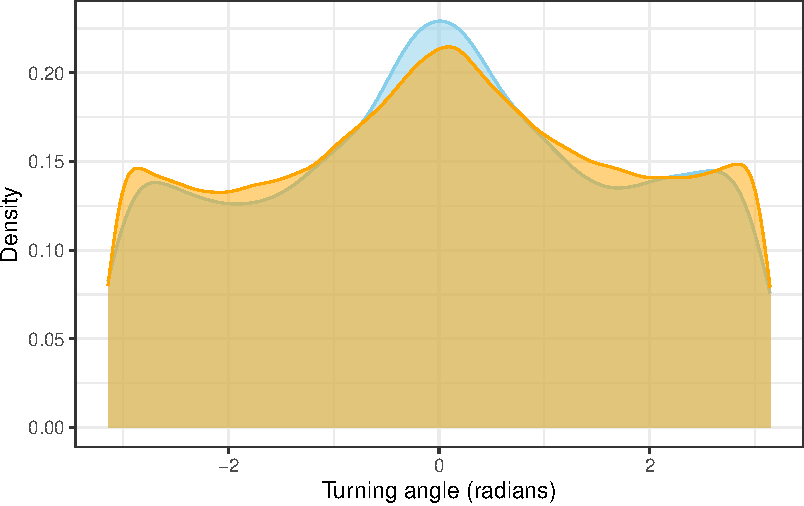
\includegraphics[keepaspectratio]{deepSSF_assessing_trajectories_files/figure-pdf/unnamed-chunk-13-1.pdf}}

\begin{Shaded}
\begin{Highlighting}[]
\FunctionTok{ggsave}\NormalTok{(}\FunctionTok{paste0}\NormalTok{(}\StringTok{"Python/outputs/model\_training/"}\NormalTok{,deepSSF\_dir,}\StringTok{"/turning\_angles.png"}\NormalTok{), }\AttributeTok{width=}\DecValTok{120}\NormalTok{, }\AttributeTok{height=}\DecValTok{80}\NormalTok{, }\AttributeTok{units=}\StringTok{"mm"}\NormalTok{, }\AttributeTok{dpi =} \DecValTok{600}\NormalTok{)}
\end{Highlighting}
\end{Shaded}

\begin{verbatim}
Warning: Removed 1 row containing non-finite outside the scale range (`stat_density()`).
Removed 101 rows containing non-finite outside the scale range
(`stat_density()`).
\end{verbatim}

\subsection{Density of step lengths for each
hour}\label{density-of-step-lengths-for-each-hour}

\begin{Shaded}
\begin{Highlighting}[]
\ControlFlowTok{for}\NormalTok{(i }\ControlFlowTok{in} \DecValTok{0}\SpecialCharTok{:}\DecValTok{23}\NormalTok{) \{}
  \FunctionTok{print}\NormalTok{(}\FunctionTok{ggplot}\NormalTok{() }\SpecialCharTok{+}
    \FunctionTok{geom\_density}\NormalTok{(}\AttributeTok{data =}\NormalTok{ all\_data }\SpecialCharTok{\%\textgreater{}\%} \FunctionTok{filter}\NormalTok{(id }\SpecialCharTok{==} \DecValTok{2005} \SpecialCharTok{\&}\NormalTok{ hour\_t1 }\SpecialCharTok{==}\NormalTok{ i),}
                 \FunctionTok{aes}\NormalTok{(}\AttributeTok{x =}\NormalTok{ sl),}
                 \AttributeTok{fill =} \StringTok{"skyblue"}\NormalTok{, }\AttributeTok{colour =} \StringTok{"black"}\NormalTok{, }\AttributeTok{alpha =} \FloatTok{0.5}\NormalTok{) }\SpecialCharTok{+}
    \FunctionTok{geom\_density}\NormalTok{(}\AttributeTok{data =}\NormalTok{ all\_data }\SpecialCharTok{\%\textgreater{}\%} \FunctionTok{filter}\NormalTok{(}\SpecialCharTok{!}\NormalTok{id }\SpecialCharTok{==} \DecValTok{2005} \SpecialCharTok{\&}\NormalTok{ hour\_t1 }\SpecialCharTok{==}\NormalTok{ i),}
                 \FunctionTok{aes}\NormalTok{(}\AttributeTok{x =}\NormalTok{ sl),}
                 \AttributeTok{fill =} \StringTok{"orange"}\NormalTok{, }\AttributeTok{colour =} \StringTok{"black"}\NormalTok{, }\AttributeTok{alpha =} \FloatTok{0.5}\NormalTok{) }\SpecialCharTok{+}
      \FunctionTok{scale\_x\_continuous}\NormalTok{(}\StringTok{"Step length (m)"}\NormalTok{, }\AttributeTok{limits =} \FunctionTok{c}\NormalTok{(}\DecValTok{0}\NormalTok{, }\DecValTok{1500}\NormalTok{)) }\SpecialCharTok{+}
      \FunctionTok{ggtitle}\NormalTok{(}\FunctionTok{paste0}\NormalTok{(}\StringTok{"Hour: "}\NormalTok{, i)) }\SpecialCharTok{+}
    \FunctionTok{theme\_bw}\NormalTok{())}
\NormalTok{\}}
\end{Highlighting}
\end{Shaded}

\begin{verbatim}
Warning: Removed 3 rows containing non-finite outside the scale range
(`stat_density()`).
\end{verbatim}

\begin{verbatim}
Warning: Removed 52 rows containing non-finite outside the scale range
(`stat_density()`).
\end{verbatim}

\pandocbounded{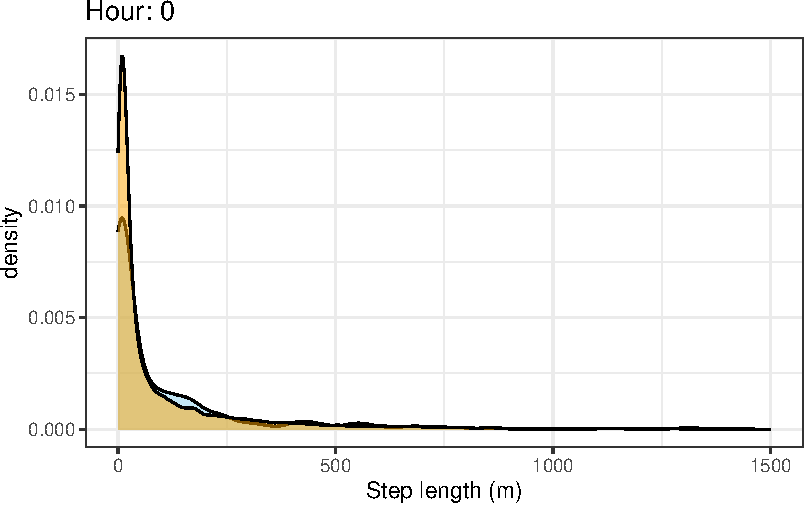
\includegraphics[keepaspectratio]{deepSSF_assessing_trajectories_files/figure-pdf/unnamed-chunk-14-1.pdf}}

\begin{verbatim}
Warning: Removed 5 rows containing non-finite outside the scale range
(`stat_density()`).
\end{verbatim}

\begin{verbatim}
Warning: Removed 35 rows containing non-finite outside the scale range
(`stat_density()`).
\end{verbatim}

\pandocbounded{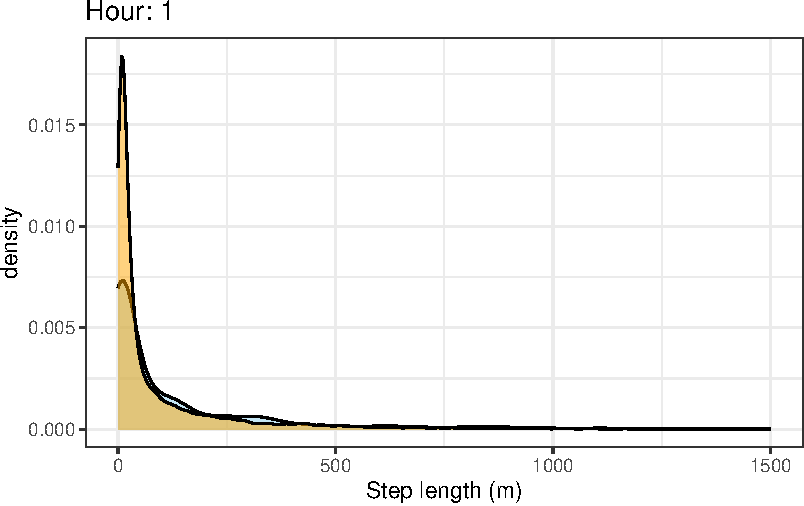
\includegraphics[keepaspectratio]{deepSSF_assessing_trajectories_files/figure-pdf/unnamed-chunk-14-2.pdf}}

\begin{verbatim}
Warning: Removed 5 rows containing non-finite outside the scale range
(`stat_density()`).
\end{verbatim}

\begin{verbatim}
Warning: Removed 36 rows containing non-finite outside the scale range
(`stat_density()`).
\end{verbatim}

\pandocbounded{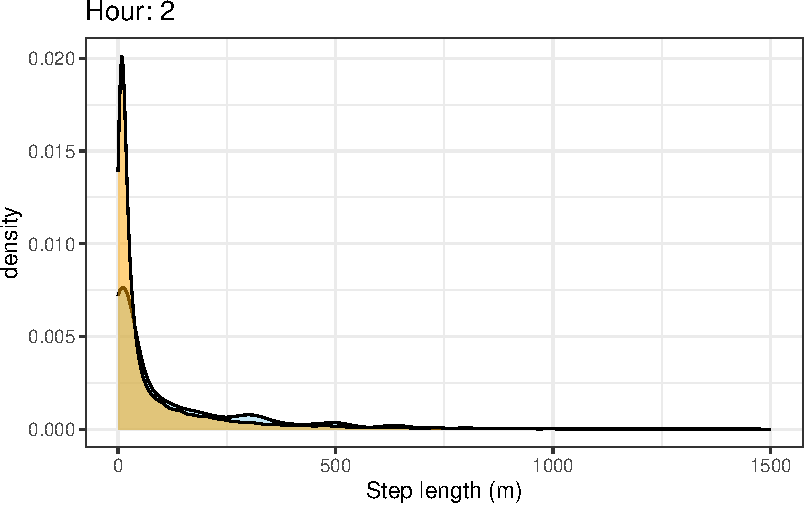
\includegraphics[keepaspectratio]{deepSSF_assessing_trajectories_files/figure-pdf/unnamed-chunk-14-3.pdf}}

\begin{verbatim}
Warning: Removed 6 rows containing non-finite outside the scale range
(`stat_density()`).
\end{verbatim}

\begin{verbatim}
Warning: Removed 39 rows containing non-finite outside the scale range
(`stat_density()`).
\end{verbatim}

\pandocbounded{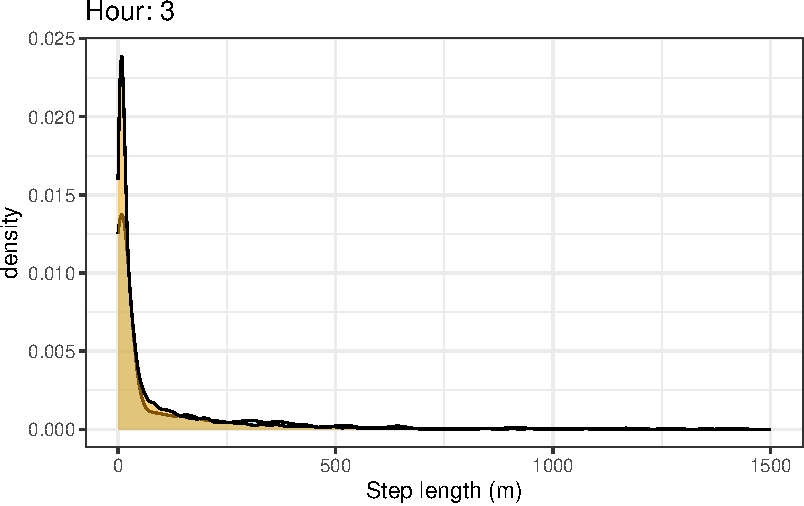
\includegraphics[keepaspectratio]{deepSSF_assessing_trajectories_files/figure-pdf/unnamed-chunk-14-4.pdf}}

\begin{verbatim}
Warning: Removed 2 rows containing non-finite outside the scale range
(`stat_density()`).
Removed 39 rows containing non-finite outside the scale range
(`stat_density()`).
\end{verbatim}

\pandocbounded{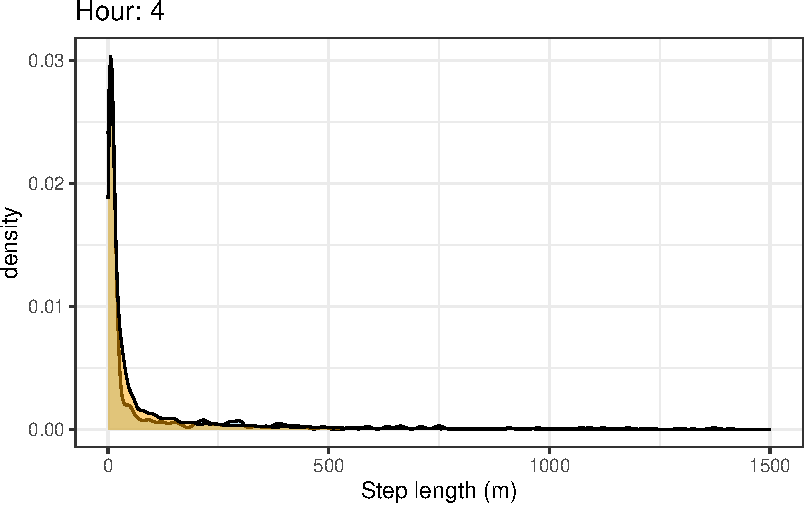
\includegraphics[keepaspectratio]{deepSSF_assessing_trajectories_files/figure-pdf/unnamed-chunk-14-5.pdf}}

\begin{verbatim}
Warning: Removed 7 rows containing non-finite outside the scale range
(`stat_density()`).
\end{verbatim}

\begin{verbatim}
Warning: Removed 78 rows containing non-finite outside the scale range
(`stat_density()`).
\end{verbatim}

\pandocbounded{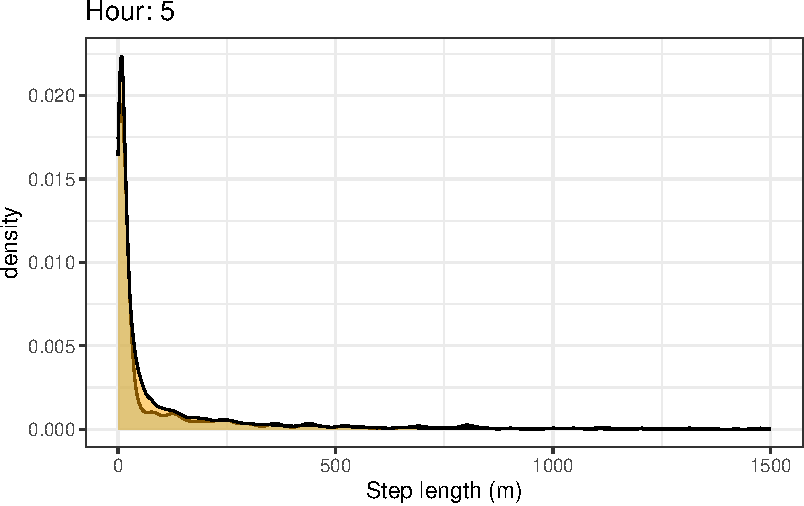
\includegraphics[keepaspectratio]{deepSSF_assessing_trajectories_files/figure-pdf/unnamed-chunk-14-6.pdf}}

\begin{verbatim}
Warning: Removed 12 rows containing non-finite outside the scale range
(`stat_density()`).
\end{verbatim}

\begin{verbatim}
Warning: Removed 199 rows containing non-finite outside the scale range
(`stat_density()`).
\end{verbatim}

\pandocbounded{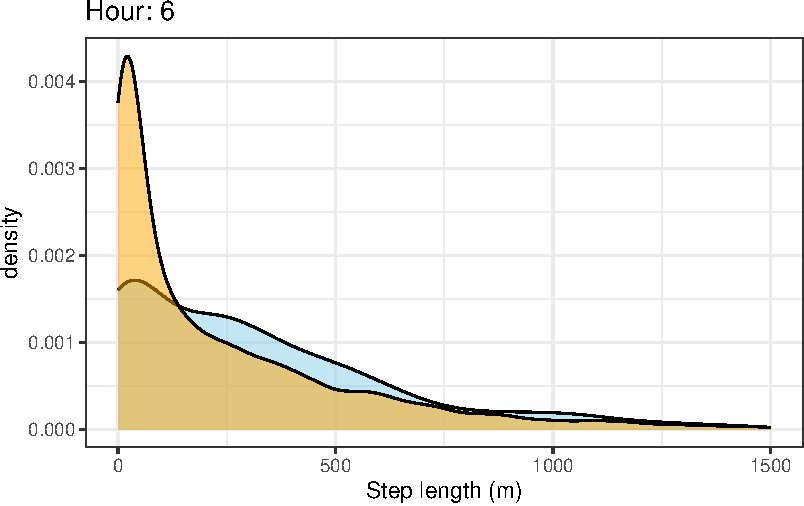
\includegraphics[keepaspectratio]{deepSSF_assessing_trajectories_files/figure-pdf/unnamed-chunk-14-7.pdf}}

\begin{verbatim}
Warning: Removed 15 rows containing non-finite outside the scale range
(`stat_density()`).
\end{verbatim}

\begin{verbatim}
Warning: Removed 320 rows containing non-finite outside the scale range
(`stat_density()`).
\end{verbatim}

\pandocbounded{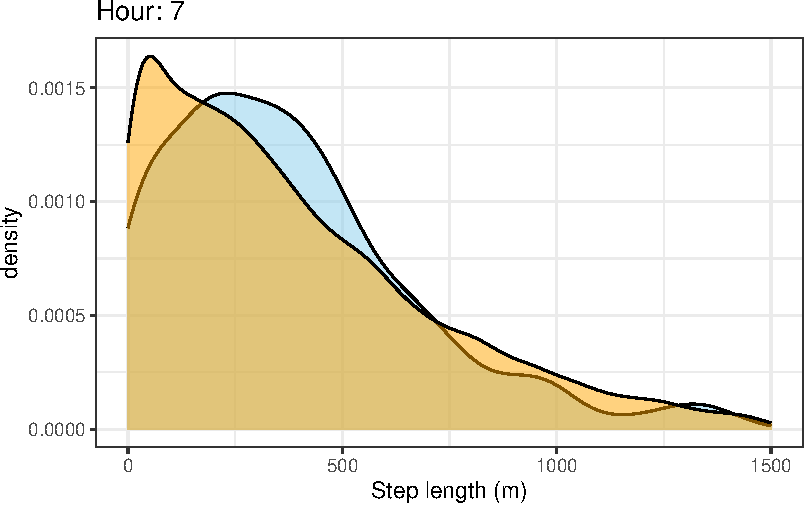
\includegraphics[keepaspectratio]{deepSSF_assessing_trajectories_files/figure-pdf/unnamed-chunk-14-8.pdf}}

\begin{verbatim}
Warning: Removed 18 rows containing non-finite outside the scale range
(`stat_density()`).
\end{verbatim}

\begin{verbatim}
Warning: Removed 377 rows containing non-finite outside the scale range
(`stat_density()`).
\end{verbatim}

\pandocbounded{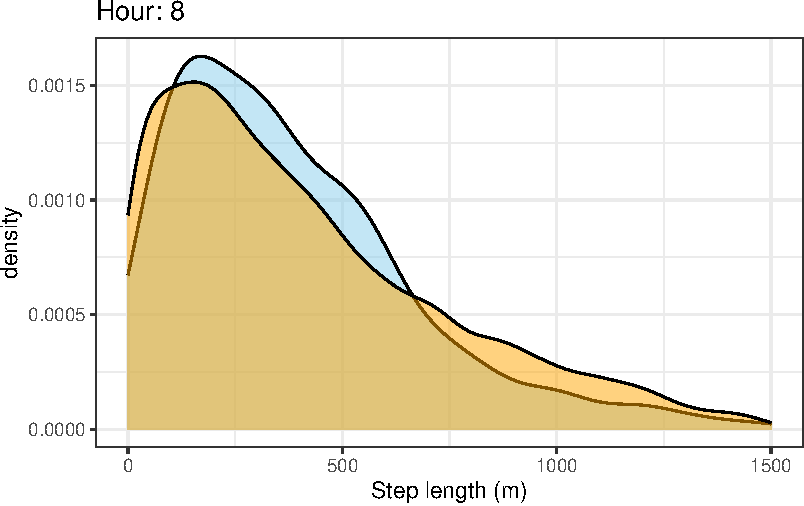
\includegraphics[keepaspectratio]{deepSSF_assessing_trajectories_files/figure-pdf/unnamed-chunk-14-9.pdf}}

\begin{verbatim}
Warning: Removed 6 rows containing non-finite outside the scale range
(`stat_density()`).
\end{verbatim}

\begin{verbatim}
Warning: Removed 266 rows containing non-finite outside the scale range
(`stat_density()`).
\end{verbatim}

\pandocbounded{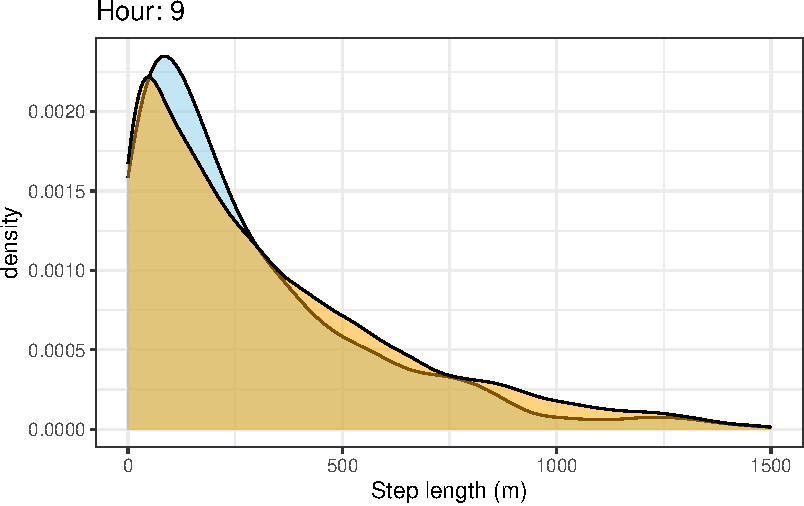
\includegraphics[keepaspectratio]{deepSSF_assessing_trajectories_files/figure-pdf/unnamed-chunk-14-10.pdf}}

\begin{verbatim}
Warning: Removed 3 rows containing non-finite outside the scale range
(`stat_density()`).
\end{verbatim}

\begin{verbatim}
Warning: Removed 164 rows containing non-finite outside the scale range
(`stat_density()`).
\end{verbatim}

\pandocbounded{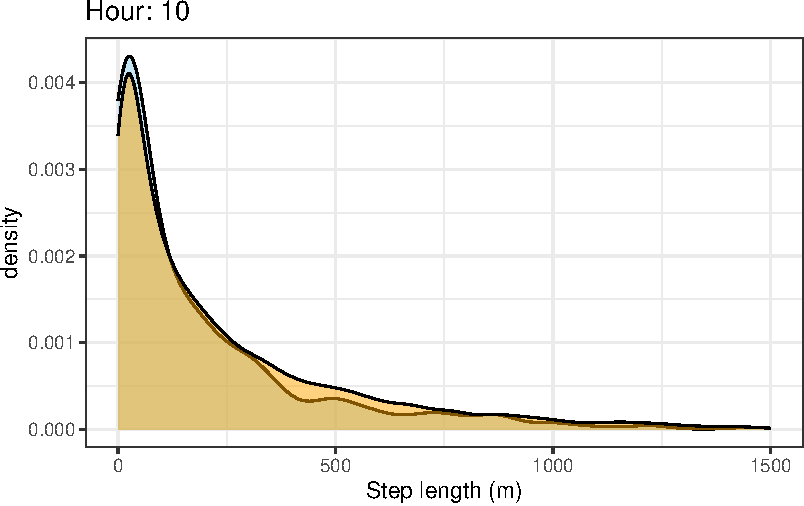
\includegraphics[keepaspectratio]{deepSSF_assessing_trajectories_files/figure-pdf/unnamed-chunk-14-11.pdf}}

\begin{verbatim}
Warning: Removed 2 rows containing non-finite outside the scale range
(`stat_density()`).
\end{verbatim}

\begin{verbatim}
Warning: Removed 88 rows containing non-finite outside the scale range
(`stat_density()`).
\end{verbatim}

\pandocbounded{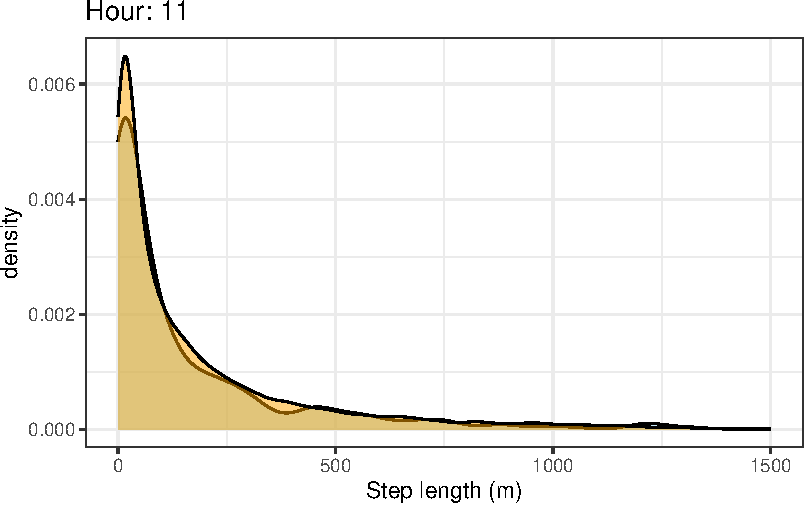
\includegraphics[keepaspectratio]{deepSSF_assessing_trajectories_files/figure-pdf/unnamed-chunk-14-12.pdf}}

\begin{verbatim}
Warning: Removed 1 row containing non-finite outside the scale range
(`stat_density()`).
\end{verbatim}

\begin{verbatim}
Warning: Removed 44 rows containing non-finite outside the scale range
(`stat_density()`).
\end{verbatim}

\pandocbounded{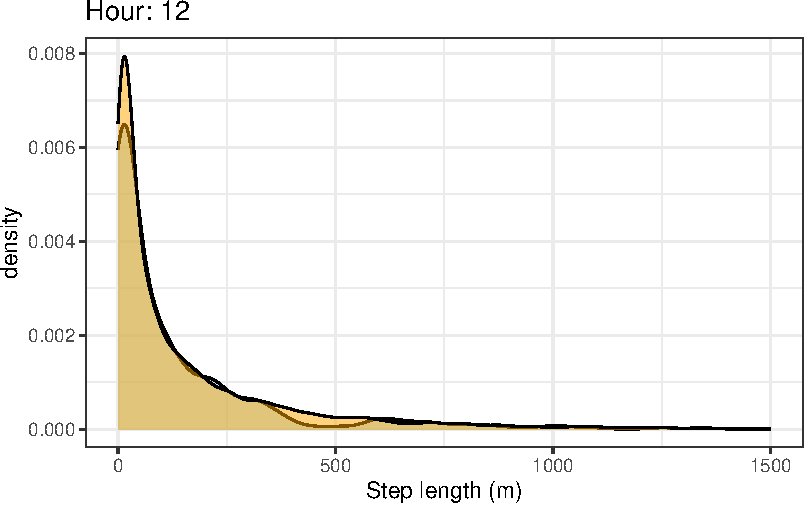
\includegraphics[keepaspectratio]{deepSSF_assessing_trajectories_files/figure-pdf/unnamed-chunk-14-13.pdf}}

\begin{verbatim}
Warning: Removed 1 row containing non-finite outside the scale range
(`stat_density()`).
\end{verbatim}

\begin{verbatim}
Warning: Removed 54 rows containing non-finite outside the scale range
(`stat_density()`).
\end{verbatim}

\pandocbounded{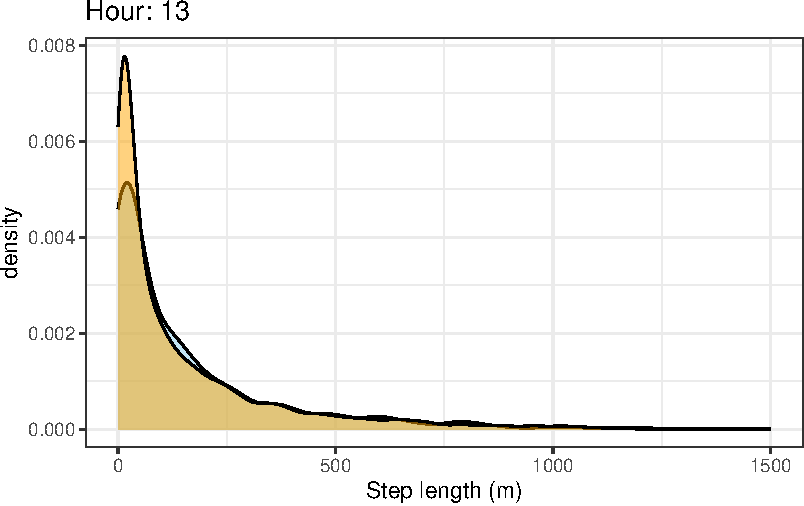
\includegraphics[keepaspectratio]{deepSSF_assessing_trajectories_files/figure-pdf/unnamed-chunk-14-14.pdf}}

\begin{verbatim}
Warning: Removed 3 rows containing non-finite outside the scale range
(`stat_density()`).
\end{verbatim}

\begin{verbatim}
Warning: Removed 57 rows containing non-finite outside the scale range
(`stat_density()`).
\end{verbatim}

\pandocbounded{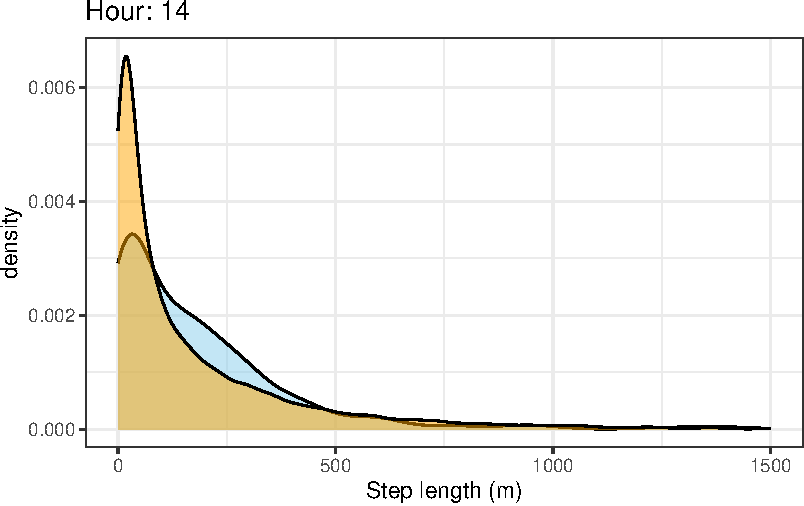
\includegraphics[keepaspectratio]{deepSSF_assessing_trajectories_files/figure-pdf/unnamed-chunk-14-15.pdf}}

\begin{verbatim}
Warning: Removed 7 rows containing non-finite outside the scale range
(`stat_density()`).
\end{verbatim}

\begin{verbatim}
Warning: Removed 74 rows containing non-finite outside the scale range
(`stat_density()`).
\end{verbatim}

\pandocbounded{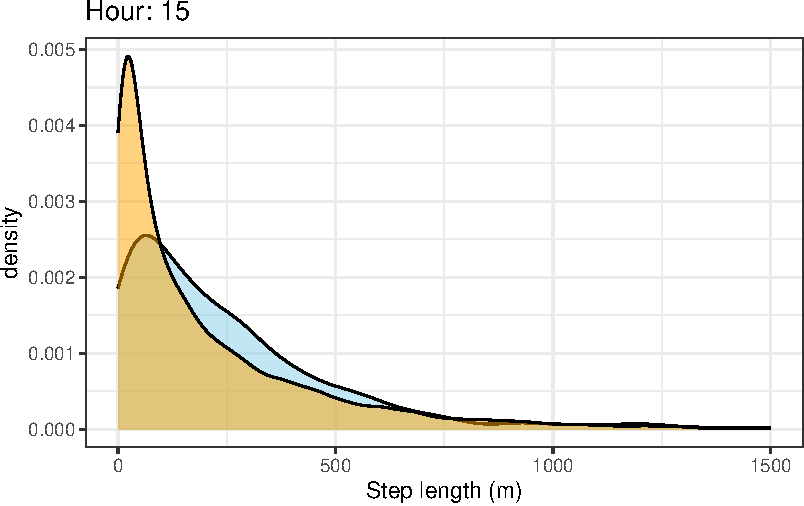
\includegraphics[keepaspectratio]{deepSSF_assessing_trajectories_files/figure-pdf/unnamed-chunk-14-16.pdf}}

\begin{verbatim}
Warning: Removed 8 rows containing non-finite outside the scale range
(`stat_density()`).
\end{verbatim}

\begin{verbatim}
Warning: Removed 161 rows containing non-finite outside the scale range
(`stat_density()`).
\end{verbatim}

\pandocbounded{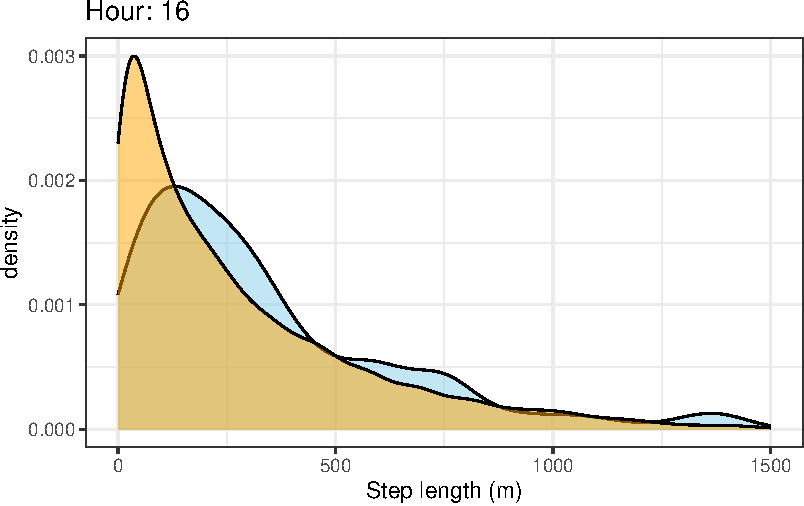
\includegraphics[keepaspectratio]{deepSSF_assessing_trajectories_files/figure-pdf/unnamed-chunk-14-17.pdf}}

\begin{verbatim}
Warning: Removed 9 rows containing non-finite outside the scale range
(`stat_density()`).
\end{verbatim}

\begin{verbatim}
Warning: Removed 273 rows containing non-finite outside the scale range
(`stat_density()`).
\end{verbatim}

\pandocbounded{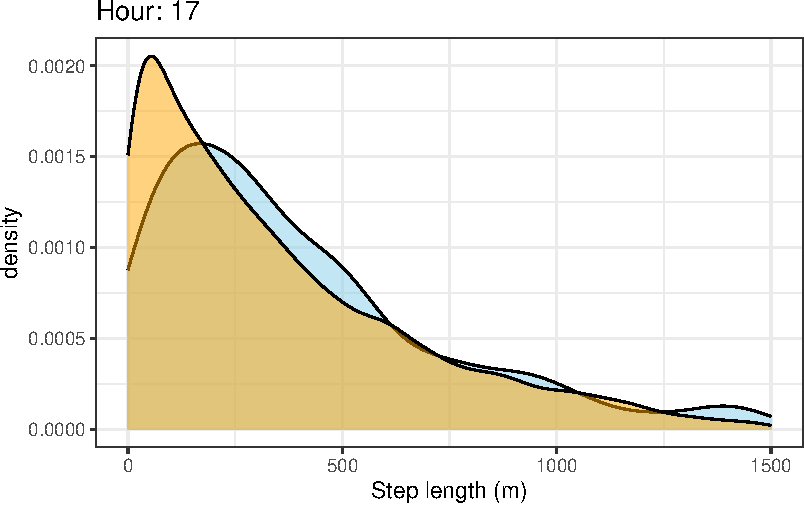
\includegraphics[keepaspectratio]{deepSSF_assessing_trajectories_files/figure-pdf/unnamed-chunk-14-18.pdf}}

\begin{verbatim}
Warning: Removed 12 rows containing non-finite outside the scale range
(`stat_density()`).
\end{verbatim}

\begin{verbatim}
Warning: Removed 398 rows containing non-finite outside the scale range
(`stat_density()`).
\end{verbatim}

\pandocbounded{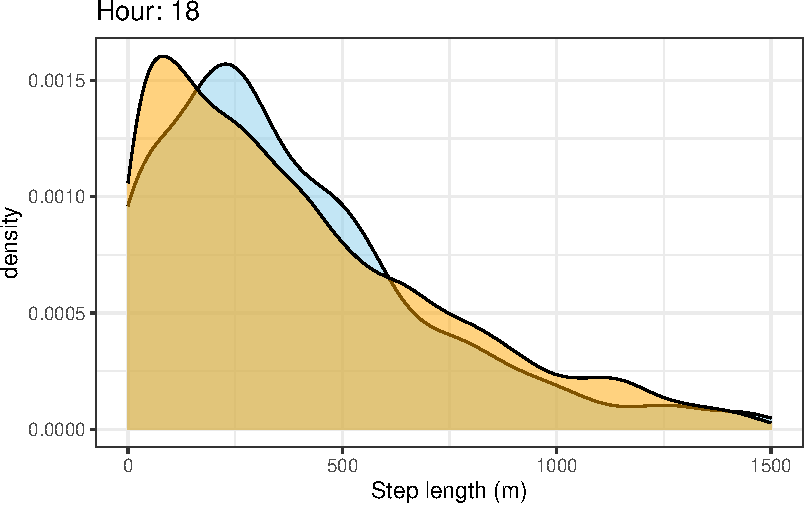
\includegraphics[keepaspectratio]{deepSSF_assessing_trajectories_files/figure-pdf/unnamed-chunk-14-19.pdf}}

\begin{verbatim}
Warning: Removed 9 rows containing non-finite outside the scale range
(`stat_density()`).
\end{verbatim}

\begin{verbatim}
Warning: Removed 457 rows containing non-finite outside the scale range
(`stat_density()`).
\end{verbatim}

\pandocbounded{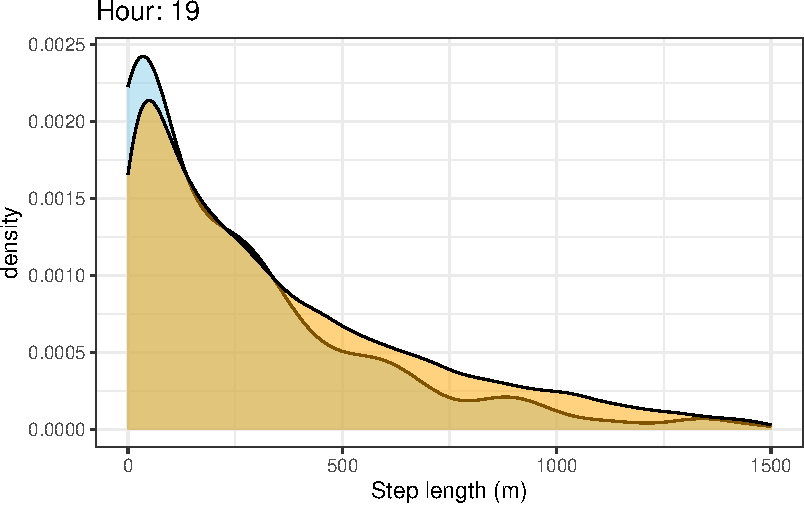
\includegraphics[keepaspectratio]{deepSSF_assessing_trajectories_files/figure-pdf/unnamed-chunk-14-20.pdf}}

\begin{verbatim}
Warning: Removed 5 rows containing non-finite outside the scale range
(`stat_density()`).
\end{verbatim}

\begin{verbatim}
Warning: Removed 228 rows containing non-finite outside the scale range
(`stat_density()`).
\end{verbatim}

\pandocbounded{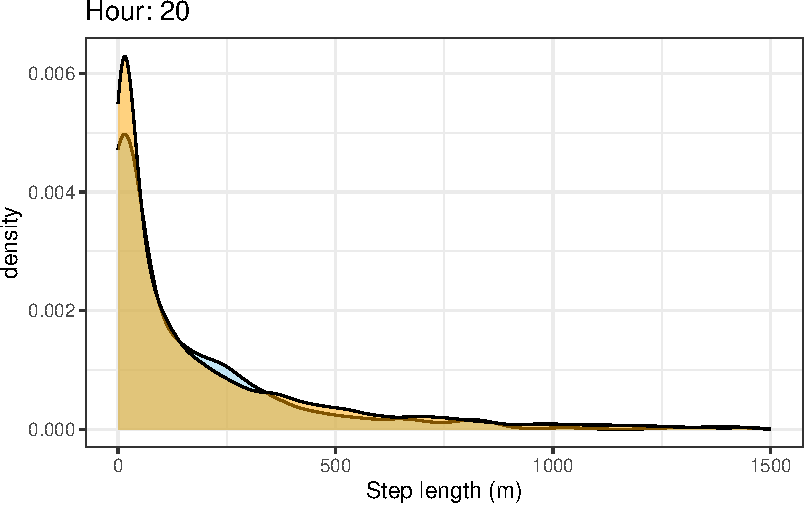
\includegraphics[keepaspectratio]{deepSSF_assessing_trajectories_files/figure-pdf/unnamed-chunk-14-21.pdf}}

\begin{verbatim}
Warning: Removed 3 rows containing non-finite outside the scale range
(`stat_density()`).
\end{verbatim}

\begin{verbatim}
Warning: Removed 103 rows containing non-finite outside the scale range
(`stat_density()`).
\end{verbatim}

\pandocbounded{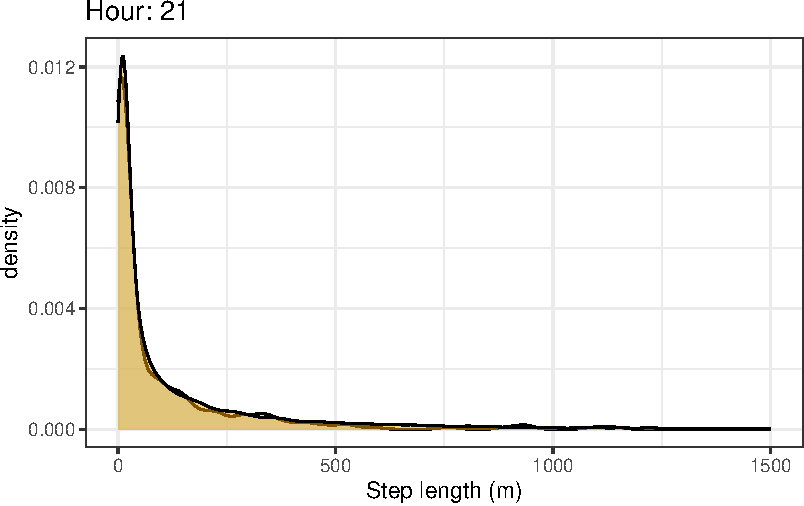
\includegraphics[keepaspectratio]{deepSSF_assessing_trajectories_files/figure-pdf/unnamed-chunk-14-22.pdf}}

\begin{verbatim}
Warning: Removed 2 rows containing non-finite outside the scale range
(`stat_density()`).
\end{verbatim}

\begin{verbatim}
Warning: Removed 60 rows containing non-finite outside the scale range
(`stat_density()`).
\end{verbatim}

\pandocbounded{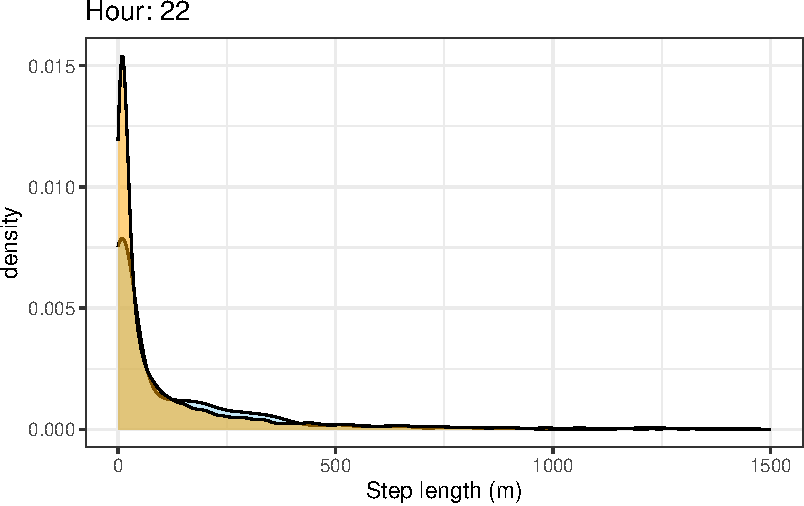
\includegraphics[keepaspectratio]{deepSSF_assessing_trajectories_files/figure-pdf/unnamed-chunk-14-23.pdf}}

\begin{verbatim}
Warning: Removed 3 rows containing non-finite outside the scale range
(`stat_density()`).
\end{verbatim}

\begin{verbatim}
Warning: Removed 101 rows containing non-finite outside the scale range
(`stat_density()`).
\end{verbatim}

\pandocbounded{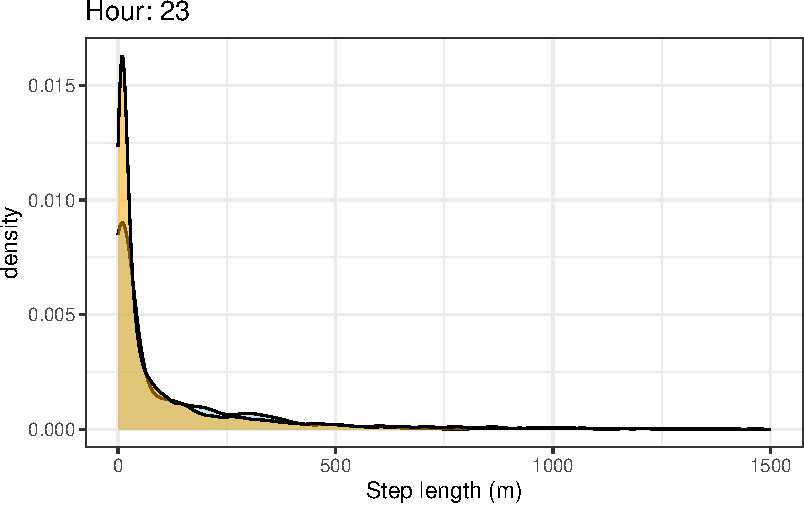
\includegraphics[keepaspectratio]{deepSSF_assessing_trajectories_files/figure-pdf/unnamed-chunk-14-24.pdf}}

\subsection{Density of turning angles for each
hour}\label{density-of-turning-angles-for-each-hour}

\begin{Shaded}
\begin{Highlighting}[]
\ControlFlowTok{for}\NormalTok{(i }\ControlFlowTok{in} \DecValTok{0}\SpecialCharTok{:}\DecValTok{23}\NormalTok{) \{}
  \FunctionTok{print}\NormalTok{(}\FunctionTok{ggplot}\NormalTok{() }\SpecialCharTok{+}
    \FunctionTok{geom\_density}\NormalTok{(}\AttributeTok{data =}\NormalTok{ all\_data }\SpecialCharTok{\%\textgreater{}\%} \FunctionTok{filter}\NormalTok{(id }\SpecialCharTok{==} \DecValTok{2005} \SpecialCharTok{\&}\NormalTok{ hour\_t1 }\SpecialCharTok{==}\NormalTok{ i),}
           \FunctionTok{aes}\NormalTok{(}\AttributeTok{x =}\NormalTok{ ta),}
           \AttributeTok{fill =} \StringTok{"skyblue"}\NormalTok{, }\AttributeTok{colour =} \StringTok{"black"}\NormalTok{, }\AttributeTok{alpha =} \FloatTok{0.5}\NormalTok{) }\SpecialCharTok{+}
    \FunctionTok{geom\_density}\NormalTok{(}\AttributeTok{data =}\NormalTok{ all\_data }\SpecialCharTok{\%\textgreater{}\%} \FunctionTok{filter}\NormalTok{(}\SpecialCharTok{!}\NormalTok{id }\SpecialCharTok{==} \DecValTok{2005} \SpecialCharTok{\&}\NormalTok{ hour\_t1 }\SpecialCharTok{==}\NormalTok{ i),}
                   \FunctionTok{aes}\NormalTok{(}\AttributeTok{x =}\NormalTok{ ta),}
                 \AttributeTok{fill =} \StringTok{"orange"}\NormalTok{, }\AttributeTok{colour =} \StringTok{"black"}\NormalTok{, }\AttributeTok{alpha =} \FloatTok{0.5}\NormalTok{) }\SpecialCharTok{+}
      \FunctionTok{scale\_x\_continuous}\NormalTok{(}\StringTok{"Turning angle (radians)"}\NormalTok{, }\AttributeTok{limits =} \FunctionTok{c}\NormalTok{(}\SpecialCharTok{{-}}\NormalTok{pi, pi)) }\SpecialCharTok{+}
      \FunctionTok{ggtitle}\NormalTok{(}\FunctionTok{paste0}\NormalTok{(}\StringTok{"Hour: "}\NormalTok{, i)) }\SpecialCharTok{+}
    \FunctionTok{theme\_bw}\NormalTok{())}
\NormalTok{\}}
\end{Highlighting}
\end{Shaded}

\begin{verbatim}
Warning: Removed 50 rows containing non-finite outside the scale range
(`stat_density()`).
\end{verbatim}

\pandocbounded{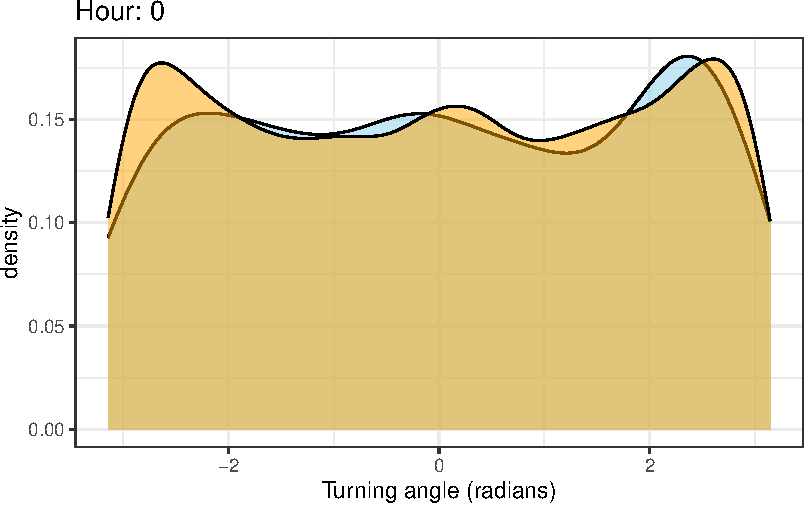
\includegraphics[keepaspectratio]{deepSSF_assessing_trajectories_files/figure-pdf/unnamed-chunk-15-1.pdf}}

\pandocbounded{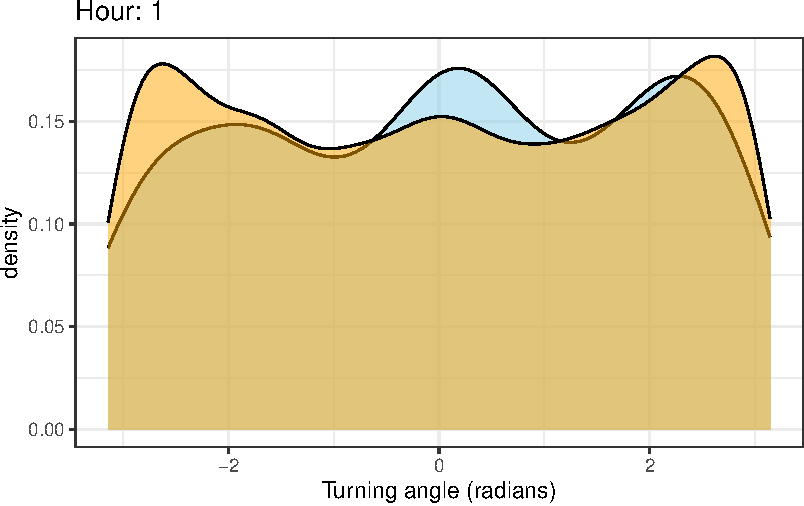
\includegraphics[keepaspectratio]{deepSSF_assessing_trajectories_files/figure-pdf/unnamed-chunk-15-2.pdf}}

\pandocbounded{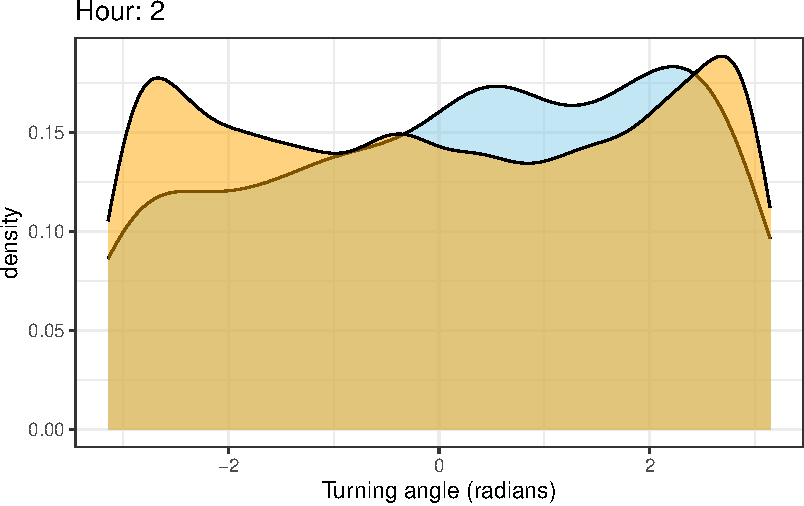
\includegraphics[keepaspectratio]{deepSSF_assessing_trajectories_files/figure-pdf/unnamed-chunk-15-3.pdf}}

\pandocbounded{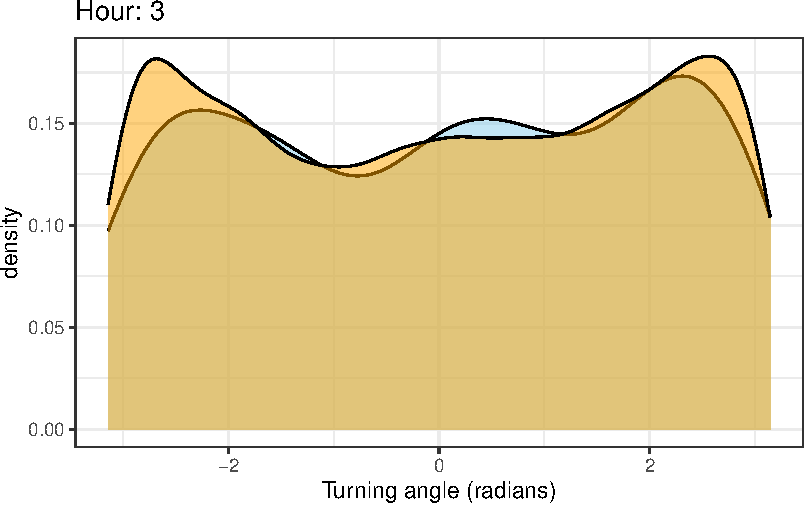
\includegraphics[keepaspectratio]{deepSSF_assessing_trajectories_files/figure-pdf/unnamed-chunk-15-4.pdf}}

\pandocbounded{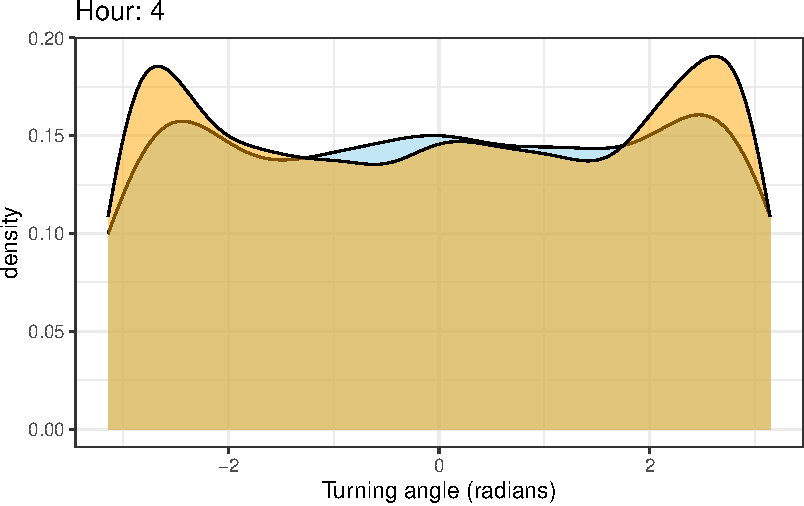
\includegraphics[keepaspectratio]{deepSSF_assessing_trajectories_files/figure-pdf/unnamed-chunk-15-5.pdf}}

\pandocbounded{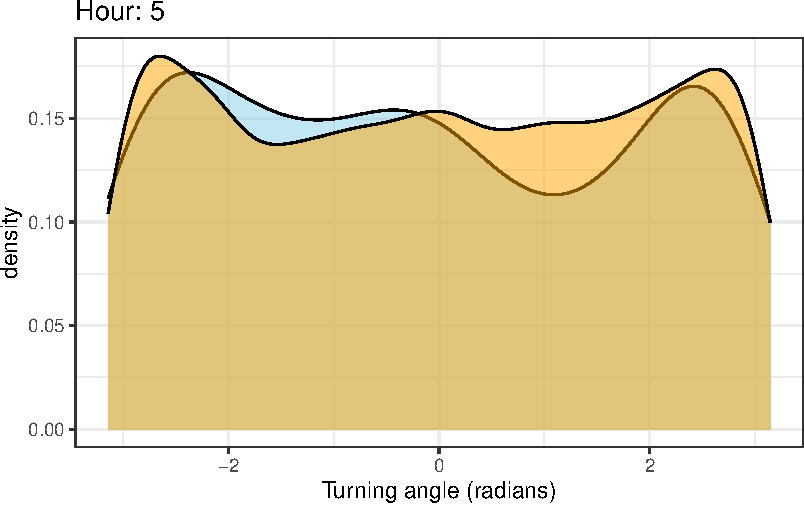
\includegraphics[keepaspectratio]{deepSSF_assessing_trajectories_files/figure-pdf/unnamed-chunk-15-6.pdf}}

\pandocbounded{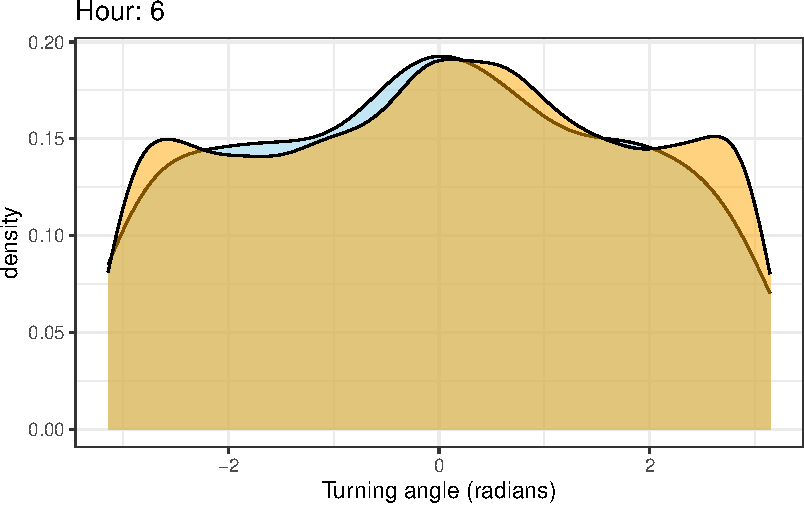
\includegraphics[keepaspectratio]{deepSSF_assessing_trajectories_files/figure-pdf/unnamed-chunk-15-7.pdf}}

\pandocbounded{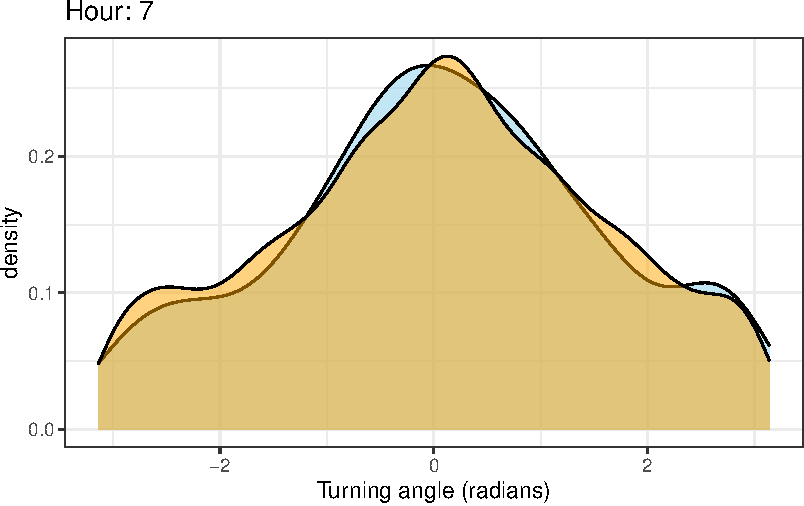
\includegraphics[keepaspectratio]{deepSSF_assessing_trajectories_files/figure-pdf/unnamed-chunk-15-8.pdf}}

\pandocbounded{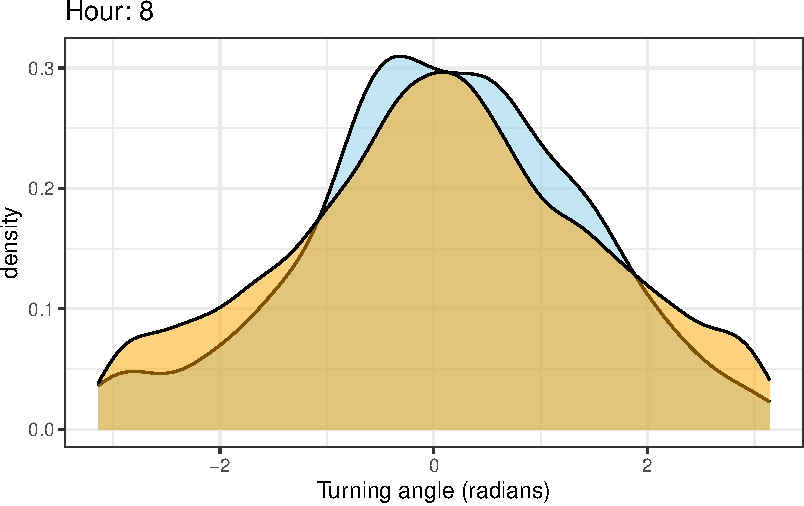
\includegraphics[keepaspectratio]{deepSSF_assessing_trajectories_files/figure-pdf/unnamed-chunk-15-9.pdf}}

\pandocbounded{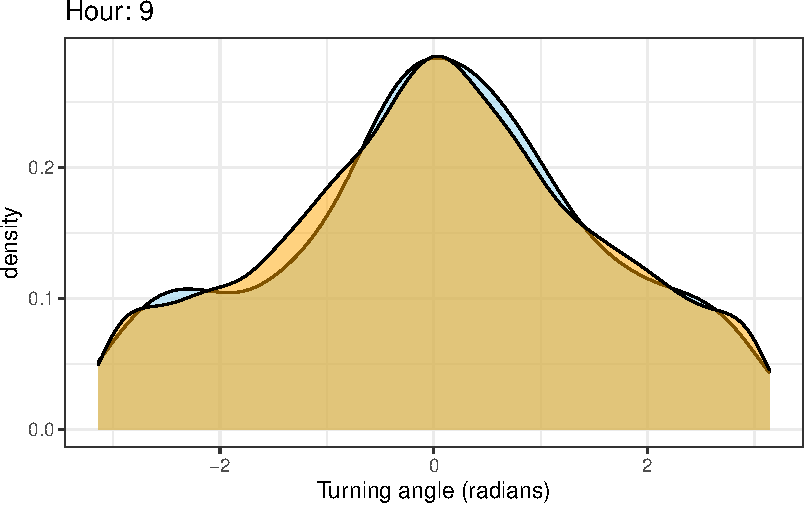
\includegraphics[keepaspectratio]{deepSSF_assessing_trajectories_files/figure-pdf/unnamed-chunk-15-10.pdf}}

\begin{verbatim}
Warning: Removed 1 row containing non-finite outside the scale range
(`stat_density()`).
\end{verbatim}

\begin{verbatim}
Warning: Removed 1 row containing non-finite outside the scale range
(`stat_density()`).
\end{verbatim}

\pandocbounded{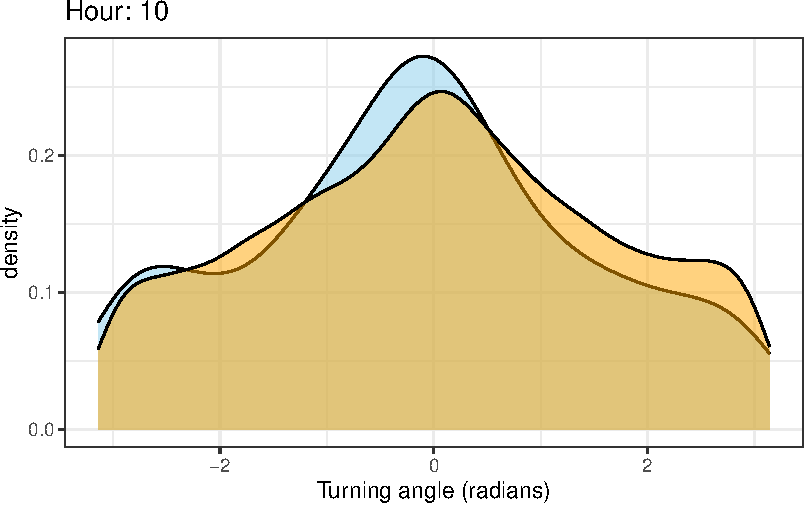
\includegraphics[keepaspectratio]{deepSSF_assessing_trajectories_files/figure-pdf/unnamed-chunk-15-11.pdf}}

\pandocbounded{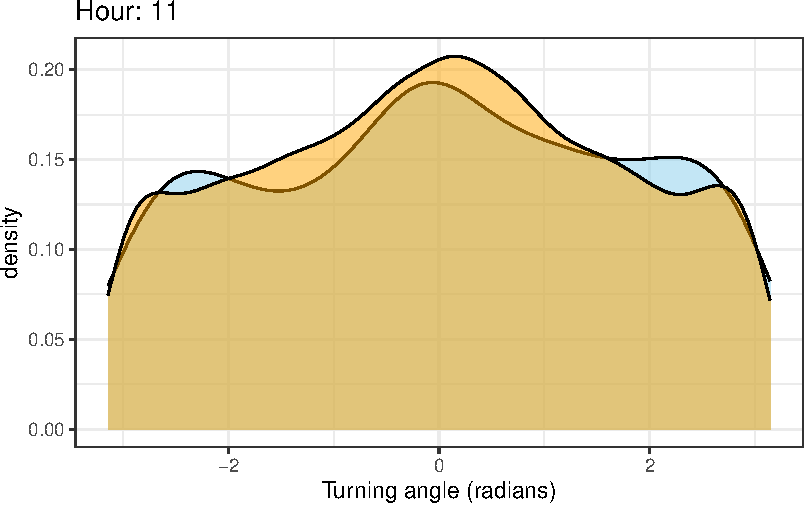
\includegraphics[keepaspectratio]{deepSSF_assessing_trajectories_files/figure-pdf/unnamed-chunk-15-12.pdf}}

\pandocbounded{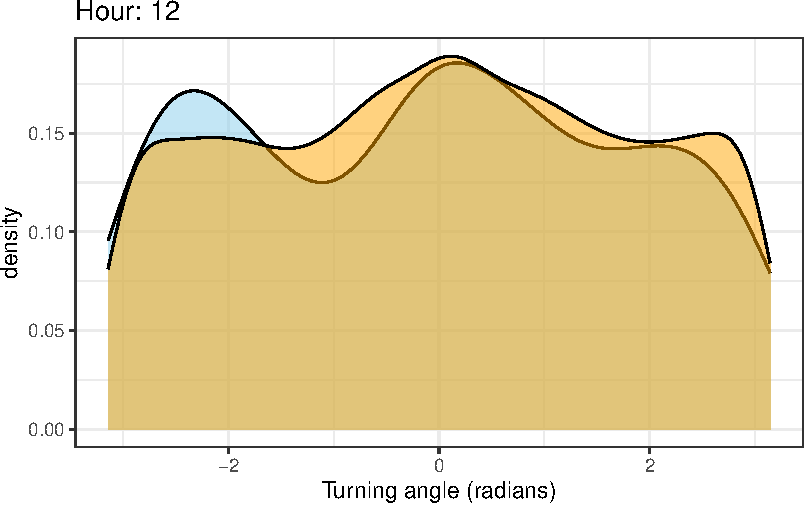
\includegraphics[keepaspectratio]{deepSSF_assessing_trajectories_files/figure-pdf/unnamed-chunk-15-13.pdf}}

\pandocbounded{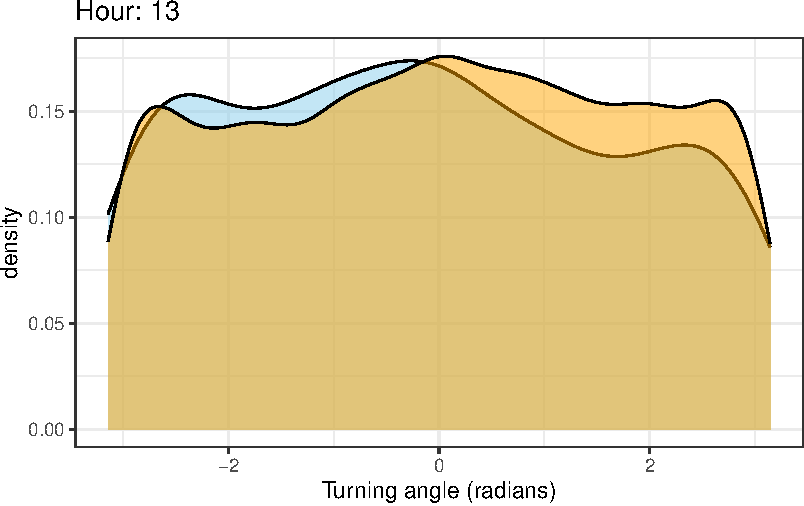
\includegraphics[keepaspectratio]{deepSSF_assessing_trajectories_files/figure-pdf/unnamed-chunk-15-14.pdf}}

\pandocbounded{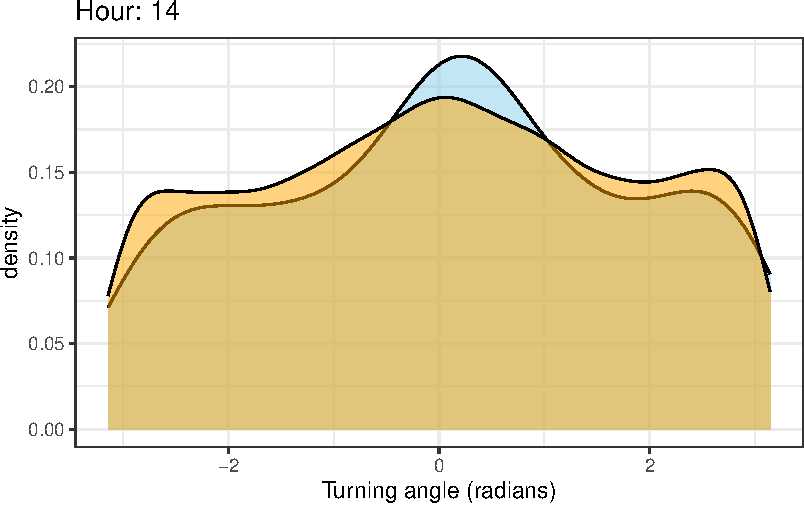
\includegraphics[keepaspectratio]{deepSSF_assessing_trajectories_files/figure-pdf/unnamed-chunk-15-15.pdf}}

\pandocbounded{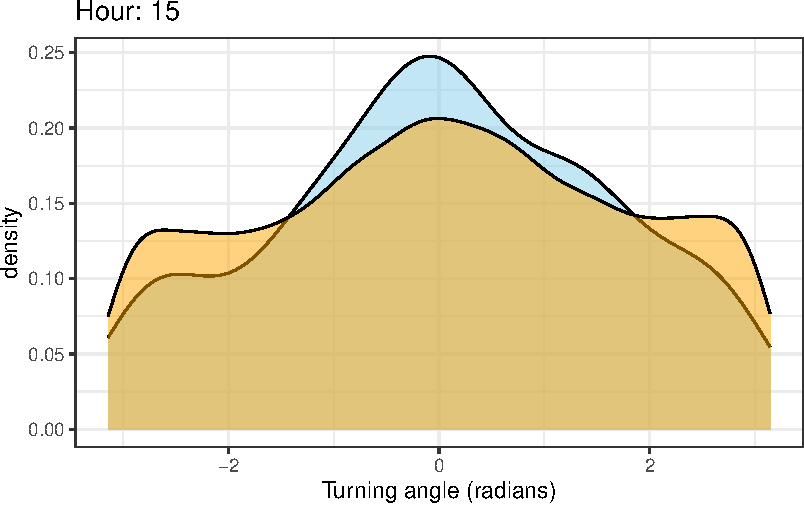
\includegraphics[keepaspectratio]{deepSSF_assessing_trajectories_files/figure-pdf/unnamed-chunk-15-16.pdf}}

\pandocbounded{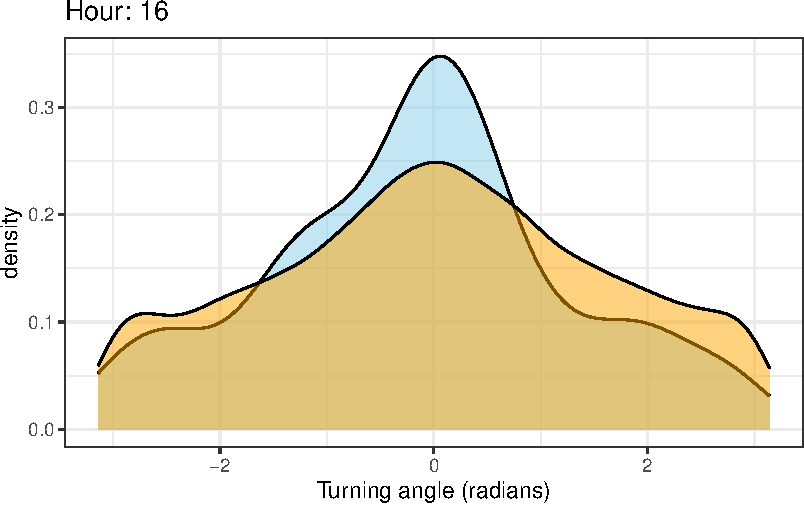
\includegraphics[keepaspectratio]{deepSSF_assessing_trajectories_files/figure-pdf/unnamed-chunk-15-17.pdf}}

\pandocbounded{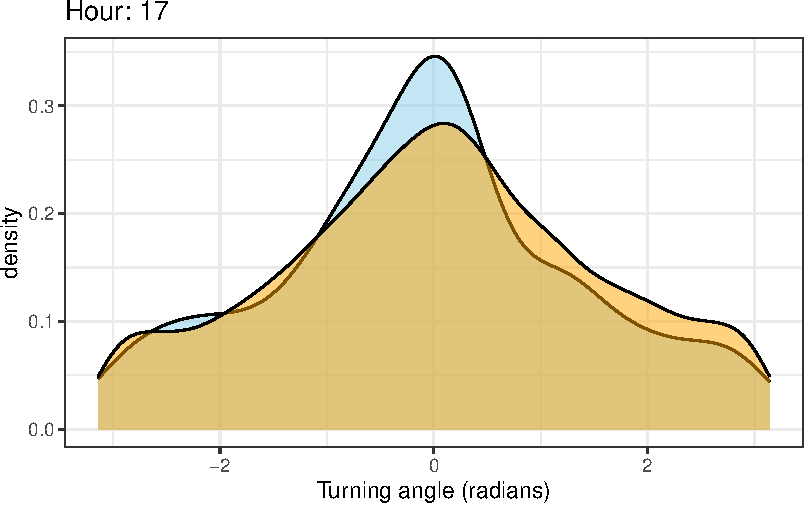
\includegraphics[keepaspectratio]{deepSSF_assessing_trajectories_files/figure-pdf/unnamed-chunk-15-18.pdf}}

\pandocbounded{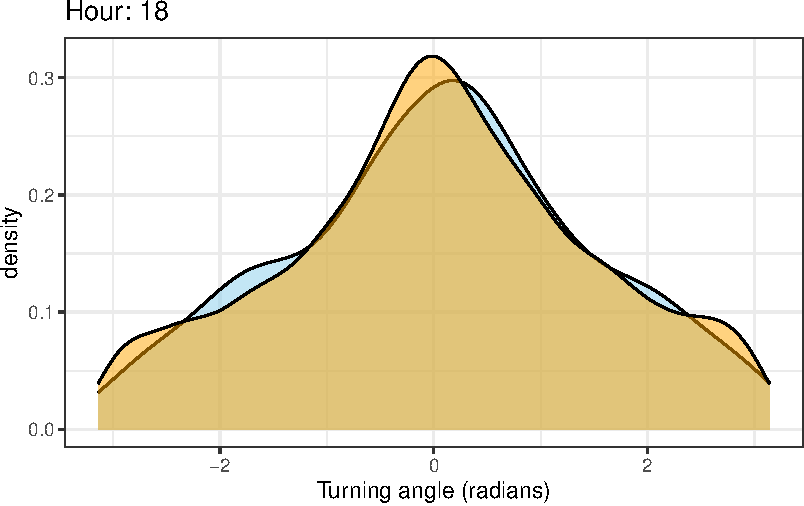
\includegraphics[keepaspectratio]{deepSSF_assessing_trajectories_files/figure-pdf/unnamed-chunk-15-19.pdf}}

\pandocbounded{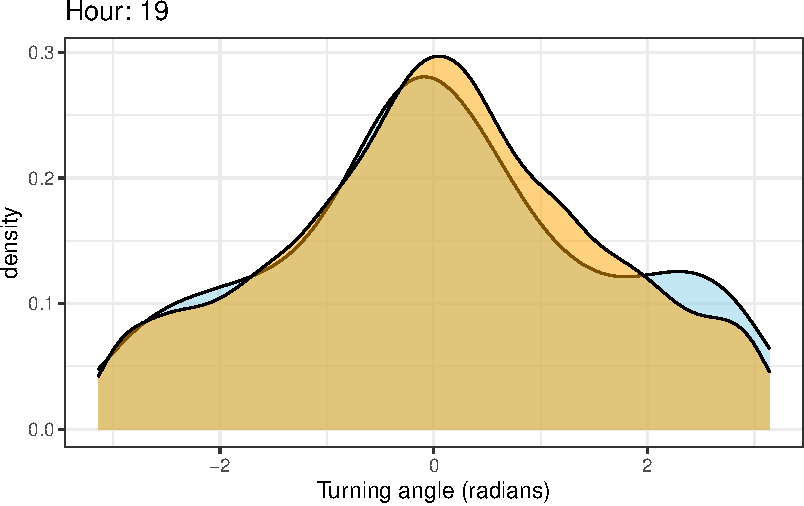
\includegraphics[keepaspectratio]{deepSSF_assessing_trajectories_files/figure-pdf/unnamed-chunk-15-20.pdf}}

\pandocbounded{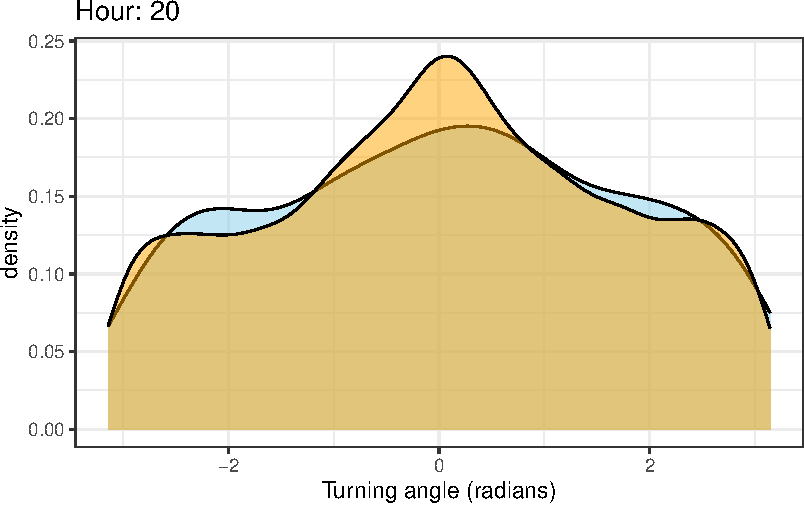
\includegraphics[keepaspectratio]{deepSSF_assessing_trajectories_files/figure-pdf/unnamed-chunk-15-21.pdf}}

\pandocbounded{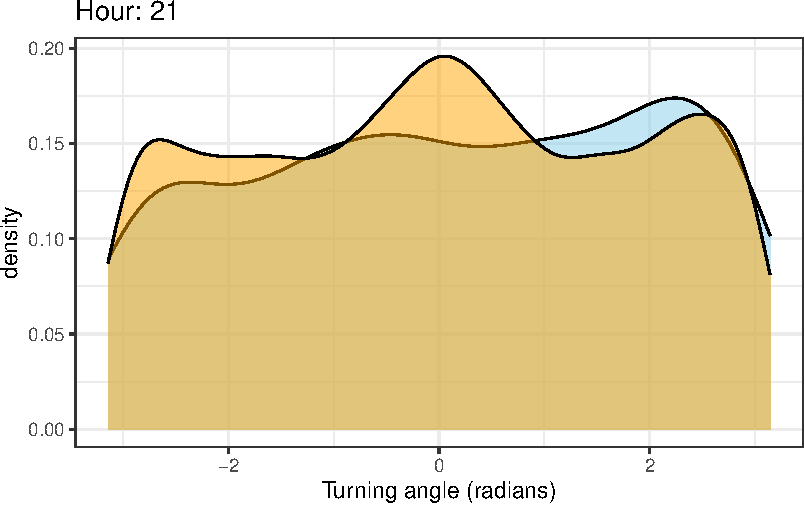
\includegraphics[keepaspectratio]{deepSSF_assessing_trajectories_files/figure-pdf/unnamed-chunk-15-22.pdf}}

\pandocbounded{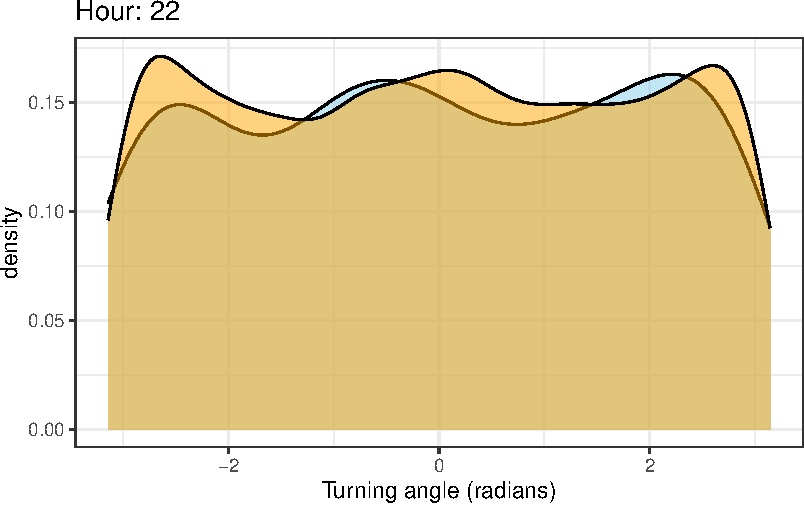
\includegraphics[keepaspectratio]{deepSSF_assessing_trajectories_files/figure-pdf/unnamed-chunk-15-23.pdf}}

\begin{verbatim}
Warning: Removed 50 rows containing non-finite outside the scale range
(`stat_density()`).
\end{verbatim}

\pandocbounded{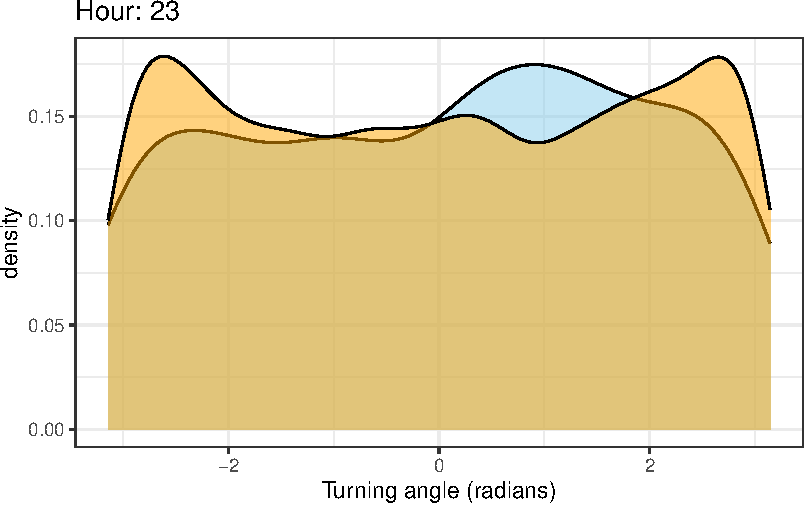
\includegraphics[keepaspectratio]{deepSSF_assessing_trajectories_files/figure-pdf/unnamed-chunk-15-24.pdf}}

\section{Extract covariate values}\label{extract-covariate-values}

To check the distribution of environmental values, we can extract the
values of the covariates at the locations of the observed and simulated
data.

We also need to index the correct NDVI raster for each row of the data.

\begin{Shaded}
\begin{Highlighting}[]
\CommentTok{\# for the simulated data}
\NormalTok{all\_data\_xy }\OtherTok{\textless{}{-}} \FunctionTok{data.frame}\NormalTok{(}\StringTok{"x"} \OtherTok{=}\NormalTok{ all\_data}\SpecialCharTok{$}\NormalTok{x1, }\StringTok{"y"} \OtherTok{=}\NormalTok{ all\_data}\SpecialCharTok{$}\NormalTok{y1)}

\CommentTok{\# Calculate ndvi\_index for all rows at once using vectorized operation}
\NormalTok{all\_data }\OtherTok{\textless{}{-}}\NormalTok{ all\_data }\SpecialCharTok{\%\textgreater{}\%}
  \FunctionTok{mutate}\NormalTok{(}
    \AttributeTok{ndvi\_index =} \FunctionTok{vapply}\NormalTok{(t1, }\ControlFlowTok{function}\NormalTok{(t) }\FunctionTok{which.min}\NormalTok{(}\FunctionTok{abs}\NormalTok{(}\FunctionTok{difftime}\NormalTok{(t, terra}\SpecialCharTok{::}\FunctionTok{time}\NormalTok{(ndvi)))), }\FunctionTok{integer}\NormalTok{(}\DecValTok{1}\NormalTok{)),}
\NormalTok{    )}

\CommentTok{\# Split row indices by the corresponding NDVI layer index}
\NormalTok{ndvi\_groups }\OtherTok{\textless{}{-}} \FunctionTok{split}\NormalTok{(}\FunctionTok{seq\_len}\NormalTok{(}\FunctionTok{nrow}\NormalTok{(all\_data\_xy)), all\_data}\SpecialCharTok{$}\NormalTok{ndvi\_index)}

\CommentTok{\# Extract values per group in one call per layer}
\NormalTok{extracted\_ndvi }\OtherTok{\textless{}{-}} \FunctionTok{map2}\NormalTok{(ndvi\_groups, }\FunctionTok{names}\NormalTok{(ndvi\_groups), }\ControlFlowTok{function}\NormalTok{(rows, index\_str) \{}
  \CommentTok{\# Convert the layer index from character to numeric if needed}
\NormalTok{  index }\OtherTok{\textless{}{-}} \FunctionTok{as.numeric}\NormalTok{(index\_str)}
\NormalTok{  terra}\SpecialCharTok{::}\FunctionTok{extract}\NormalTok{(ndvi[[index]], all\_data\_xy[rows, , }\AttributeTok{drop =} \ConstantTok{FALSE}\NormalTok{])[,}\DecValTok{2}\NormalTok{]}
\NormalTok{\})}

\CommentTok{\# Reassemble the extracted ndvi values into a single vector in original order}
\NormalTok{ndvi\_values }\OtherTok{\textless{}{-}} \FunctionTok{unsplit}\NormalTok{(extracted\_ndvi, all\_data}\SpecialCharTok{$}\NormalTok{ndvi\_index)}

\CommentTok{\# Extract raster data based on calculated ndvi\_index}
\NormalTok{all\_data }\OtherTok{\textless{}{-}}\NormalTok{ all\_data }\SpecialCharTok{\%\textgreater{}\%}
  \FunctionTok{mutate}\NormalTok{(}
    \AttributeTok{ndvi =}\NormalTok{ ndvi\_values,}
    \AttributeTok{canopy\_cover =}\NormalTok{ terra}\SpecialCharTok{::}\FunctionTok{extract}\NormalTok{(canopy\_cover, all\_data\_xy)[,}\DecValTok{2}\NormalTok{],}
    \AttributeTok{veg\_herby =}\NormalTok{ terra}\SpecialCharTok{::}\FunctionTok{extract}\NormalTok{(veg\_herby, all\_data\_xy)[,}\DecValTok{2}\NormalTok{],}
    \AttributeTok{slope =}\NormalTok{ terra}\SpecialCharTok{::}\FunctionTok{extract}\NormalTok{(slope, all\_data\_xy)[,}\DecValTok{2}\NormalTok{],}
\NormalTok{  ) }
\end{Highlighting}
\end{Shaded}

\section{Hourly movement behaviour and selection of
covariates}\label{hourly-movement-behaviour-and-selection-of-covariates}

Here we bin the trajectories into the hours of the day, and calculate
the mean, median (where appropriate) and sd values for the step lengths
and four habitat covariates.

We also save the results as a csv to compare between all of the models.

\begin{Shaded}
\begin{Highlighting}[]
\CommentTok{\# there are some NA values in the hour\_t1 column as well as the covariates}
\FunctionTok{sum}\NormalTok{(}\FunctionTok{is.na}\NormalTok{(all\_data}\SpecialCharTok{$}\NormalTok{hour\_t1))}
\end{Highlighting}
\end{Shaded}

\begin{verbatim}
[1] 0
\end{verbatim}

\begin{Shaded}
\begin{Highlighting}[]
\CommentTok{\# drop NAs}
\NormalTok{all\_data }\OtherTok{\textless{}{-}}\NormalTok{ all\_data }\SpecialCharTok{\%\textgreater{}\%}\NormalTok{ dplyr}\SpecialCharTok{::}\FunctionTok{select}\NormalTok{(}\SpecialCharTok{{-}}\NormalTok{date, }\SpecialCharTok{{-}}\NormalTok{time\_diff) }\SpecialCharTok{\%\textgreater{}\%} \FunctionTok{drop\_na}\NormalTok{()}

\NormalTok{hourly\_habitat }\OtherTok{\textless{}{-}}
\NormalTok{  all\_data }\SpecialCharTok{\%\textgreater{}\%} 
\NormalTok{  dplyr}\SpecialCharTok{::}\FunctionTok{group\_by}\NormalTok{(hour\_t1, id) }\SpecialCharTok{\%\textgreater{}\%}
    \FunctionTok{summarise}\NormalTok{(}\AttributeTok{n =} \FunctionTok{n}\NormalTok{(),}
              \AttributeTok{step\_length\_mean =} \FunctionTok{mean}\NormalTok{(sl, }\AttributeTok{na.rm =} \ConstantTok{TRUE}\NormalTok{),}
              \AttributeTok{step\_length\_median =} \FunctionTok{median}\NormalTok{(sl, }\AttributeTok{na.rm =} \ConstantTok{TRUE}\NormalTok{),}
              \AttributeTok{step\_length\_sd =} \FunctionTok{sd}\NormalTok{(sl, }\AttributeTok{na.rm =} \ConstantTok{TRUE}\NormalTok{),}
              \AttributeTok{ndvi\_mean =} \FunctionTok{mean}\NormalTok{(ndvi, }\AttributeTok{na.rm =} \ConstantTok{TRUE}\NormalTok{),}
              \AttributeTok{ndvi\_median =} \FunctionTok{median}\NormalTok{(ndvi, }\AttributeTok{na.rm =} \ConstantTok{TRUE}\NormalTok{),}
              \AttributeTok{ndvi\_sd =} \FunctionTok{sd}\NormalTok{(ndvi, }\AttributeTok{na.rm =} \ConstantTok{TRUE}\NormalTok{),}
              \AttributeTok{ndvi\_min =} \FunctionTok{min}\NormalTok{(ndvi, }\AttributeTok{na.rm =} \ConstantTok{TRUE}\NormalTok{),}
              \AttributeTok{ndvi\_max =} \FunctionTok{max}\NormalTok{(ndvi, }\AttributeTok{na.rm =} \ConstantTok{TRUE}\NormalTok{),}
              \AttributeTok{ndvi\_mean =} \FunctionTok{mean}\NormalTok{(ndvi, }\AttributeTok{na.rm =} \ConstantTok{TRUE}\NormalTok{),}
              \AttributeTok{ndvi\_median =} \FunctionTok{median}\NormalTok{(ndvi, }\AttributeTok{na.rm =} \ConstantTok{TRUE}\NormalTok{),}
              \AttributeTok{ndvi\_sd =} \FunctionTok{sd}\NormalTok{(ndvi, }\AttributeTok{na.rm =} \ConstantTok{TRUE}\NormalTok{),}
              \AttributeTok{herby\_mean =} \FunctionTok{mean}\NormalTok{(veg\_herby, }\AttributeTok{na.rm =} \ConstantTok{TRUE}\NormalTok{),}
              \AttributeTok{herby\_sd =} \FunctionTok{sd}\NormalTok{(veg\_herby, }\AttributeTok{na.rm =} \ConstantTok{TRUE}\NormalTok{),}
              \AttributeTok{canopy\_mean =} \FunctionTok{mean}\NormalTok{(canopy\_cover}\SpecialCharTok{/}\DecValTok{100}\NormalTok{, }\AttributeTok{na.rm =} \ConstantTok{TRUE}\NormalTok{),}
              \AttributeTok{canopy\_sd =} \FunctionTok{sd}\NormalTok{(canopy\_cover}\SpecialCharTok{/}\DecValTok{100}\NormalTok{, }\AttributeTok{na.rm =} \ConstantTok{TRUE}\NormalTok{),}
              \AttributeTok{canopy\_min =} \FunctionTok{min}\NormalTok{(canopy\_cover}\SpecialCharTok{/}\DecValTok{100}\NormalTok{, }\AttributeTok{na.rm =} \ConstantTok{TRUE}\NormalTok{),}
              \AttributeTok{canopy\_max =} \FunctionTok{max}\NormalTok{(canopy\_cover}\SpecialCharTok{/}\DecValTok{100}\NormalTok{, }\AttributeTok{na.rm =} \ConstantTok{TRUE}\NormalTok{),}
              \AttributeTok{slope\_mean =} \FunctionTok{mean}\NormalTok{(slope, }\AttributeTok{na.rm =} \ConstantTok{TRUE}\NormalTok{),}
              \AttributeTok{slope\_median =} \FunctionTok{median}\NormalTok{(slope, }\AttributeTok{na.rm =} \ConstantTok{TRUE}\NormalTok{),}
              \AttributeTok{slope\_sd =} \FunctionTok{sd}\NormalTok{(slope, }\AttributeTok{na.rm =} \ConstantTok{TRUE}\NormalTok{),}
              \AttributeTok{slope\_min =} \FunctionTok{min}\NormalTok{(slope, }\AttributeTok{na.rm =} \ConstantTok{TRUE}\NormalTok{),}
              \AttributeTok{slope\_max =} \FunctionTok{max}\NormalTok{(slope, }\AttributeTok{na.rm =} \ConstantTok{TRUE}\NormalTok{)}
\NormalTok{              ) }\SpecialCharTok{\%\textgreater{}\%} \FunctionTok{ungroup}\NormalTok{() }\SpecialCharTok{\%\textgreater{}\%} 
  \FunctionTok{mutate}\NormalTok{(}\AttributeTok{Data =} \FunctionTok{ifelse}\NormalTok{(id }\SpecialCharTok{==} \DecValTok{2005}\NormalTok{, }\StringTok{"Observed"}\NormalTok{, }\StringTok{"deepSSF"}\NormalTok{))}
\end{Highlighting}
\end{Shaded}

\begin{verbatim}
`summarise()` has grouped output by 'hour_t1'. You can override using the
`.groups` argument.
\end{verbatim}

Plotting the hourly habitat selection

\begin{Shaded}
\begin{Highlighting}[]
\NormalTok{hourly\_habitat\_long }\OtherTok{\textless{}{-}}\NormalTok{ hourly\_habitat }\SpecialCharTok{\%\textgreater{}\%}
  \FunctionTok{pivot\_longer}\NormalTok{(}\AttributeTok{cols =} \SpecialCharTok{!}\FunctionTok{c}\NormalTok{(Data, hour\_t1, id), }\AttributeTok{names\_to =} \StringTok{"variable"}\NormalTok{, }\AttributeTok{values\_to =} \StringTok{"value"}\NormalTok{)}
\end{Highlighting}
\end{Shaded}

To show the stochasticity of the simulations, here we show the 25th to
50th quantiles and the 2.5th to 97.5th quantiles of the data. Remember
that the `data' are the means for each hour for each trajectory, so the
quantiles are calculated across the means for each hour. We use a
dashed-line ribbon for the 95\% interval and a solid-line ribbon for the
50\% interval. We show the mean as a solid line.

This is the plotting approach that we used in the paper.

\subsection{Calculate the quantiles}\label{calculate-the-quantiles}

\begin{Shaded}
\begin{Highlighting}[]
\CommentTok{\# for all observed and simulated data}
\NormalTok{hourly\_summary\_quantiles }\OtherTok{\textless{}{-}}\NormalTok{ hourly\_habitat\_long }\SpecialCharTok{\%\textgreater{}\%} 
\NormalTok{  dplyr}\SpecialCharTok{::}\FunctionTok{group\_by}\NormalTok{(Data, hour\_t1, variable) }\SpecialCharTok{\%\textgreater{}\%} 
  \FunctionTok{summarise}\NormalTok{(}\AttributeTok{n =} \FunctionTok{n}\NormalTok{(), }
            \AttributeTok{mean =} \FunctionTok{mean}\NormalTok{(value, }\AttributeTok{na.rm =} \ConstantTok{TRUE}\NormalTok{),}
            \AttributeTok{sd =} \FunctionTok{sd}\NormalTok{(value, }\AttributeTok{na.rm =} \ConstantTok{TRUE}\NormalTok{),}
            \AttributeTok{q025 =} \FunctionTok{quantile}\NormalTok{(value, }\AttributeTok{probs =} \FloatTok{0.025}\NormalTok{, }\AttributeTok{na.rm =} \ConstantTok{TRUE}\NormalTok{), }
            \AttributeTok{q25 =} \FunctionTok{quantile}\NormalTok{(value, }\AttributeTok{probs =} \FloatTok{0.25}\NormalTok{, }\AttributeTok{na.rm =} \ConstantTok{TRUE}\NormalTok{),}
            \AttributeTok{q50 =} \FunctionTok{quantile}\NormalTok{(value, }\AttributeTok{probs =} \FloatTok{0.5}\NormalTok{, }\AttributeTok{na.rm =} \ConstantTok{TRUE}\NormalTok{), }
            \AttributeTok{q75 =} \FunctionTok{quantile}\NormalTok{(value, }\AttributeTok{probs =} \FloatTok{0.75}\NormalTok{, }\AttributeTok{na.rm =} \ConstantTok{TRUE}\NormalTok{),}
            \AttributeTok{q975 =} \FunctionTok{quantile}\NormalTok{(value, }\AttributeTok{probs =} \FloatTok{0.975}\NormalTok{, }\AttributeTok{na.rm =} \ConstantTok{TRUE}\NormalTok{))}
\end{Highlighting}
\end{Shaded}

\begin{verbatim}
`summarise()` has grouped output by 'Data', 'hour_t1'. You can override using
the `.groups` argument.
\end{verbatim}

\subsubsection{Summarise the background environmental
covariates}\label{summarise-the-background-environmental-covariates}

\begin{Shaded}
\begin{Highlighting}[]
\NormalTok{ndvi\_df }\OtherTok{\textless{}{-}}\NormalTok{ ndvi\_df }\SpecialCharTok{\%\textgreater{}\%} \FunctionTok{select}\NormalTok{(x,y,ndvi)}

\NormalTok{data\_extent }\OtherTok{\textless{}{-}} \FunctionTok{ext}\NormalTok{(plot\_extent[[}\DecValTok{1}\NormalTok{]], plot\_extent[[}\DecValTok{3}\NormalTok{]], plot\_extent[[}\DecValTok{2}\NormalTok{]], plot\_extent[[}\DecValTok{4}\NormalTok{]])}

\NormalTok{covariates\_data\_subset }\OtherTok{\textless{}{-}} \FunctionTok{c}\NormalTok{(ndvi[[}\DecValTok{8}\NormalTok{]], }
\NormalTok{                            canopy\_cover}\SpecialCharTok{/}\DecValTok{100}\NormalTok{, }
\NormalTok{                            veg\_herby, }
\NormalTok{                            slope) }\SpecialCharTok{\%\textgreater{}\%}\NormalTok{ terra}\SpecialCharTok{::}\FunctionTok{crop}\NormalTok{(data\_extent)}

\NormalTok{covariates\_data\_subset\_df }\OtherTok{\textless{}{-}} \FunctionTok{as.data.frame}\NormalTok{(covariates\_data\_subset, }\AttributeTok{xy =} \ConstantTok{TRUE}\NormalTok{) }

\NormalTok{covariate\_quantiles }\OtherTok{\textless{}{-}}\NormalTok{ covariates\_data\_subset\_df }\SpecialCharTok{\%\textgreater{}\%} 
  \FunctionTok{summarise}\NormalTok{(}
    \AttributeTok{ndvi\_q025 =} \FunctionTok{quantile}\NormalTok{(ndvi, }\AttributeTok{probs =} \FloatTok{0.025}\NormalTok{, }\AttributeTok{na.rm =} \ConstantTok{TRUE}\NormalTok{),}
    \AttributeTok{ndvi\_q25 =} \FunctionTok{quantile}\NormalTok{(ndvi, }\AttributeTok{probs =} \FloatTok{0.25}\NormalTok{, }\AttributeTok{na.rm =} \ConstantTok{TRUE}\NormalTok{),}
    \AttributeTok{ndvi\_q50 =} \FunctionTok{quantile}\NormalTok{(ndvi, }\AttributeTok{probs =} \FloatTok{0.5}\NormalTok{, }\AttributeTok{na.rm =} \ConstantTok{TRUE}\NormalTok{),}
    \AttributeTok{ndvi\_mean =} \FunctionTok{mean}\NormalTok{(ndvi, }\AttributeTok{na.rm =} \ConstantTok{TRUE}\NormalTok{),}
    \AttributeTok{ndvi\_q75 =} \FunctionTok{quantile}\NormalTok{(ndvi, }\AttributeTok{probs =} \FloatTok{0.75}\NormalTok{, }\AttributeTok{na.rm =} \ConstantTok{TRUE}\NormalTok{),}
    \AttributeTok{ndvi\_q975 =} \FunctionTok{quantile}\NormalTok{(ndvi, }\AttributeTok{probs =} \FloatTok{0.975}\NormalTok{, }\AttributeTok{na.rm =} \ConstantTok{TRUE}\NormalTok{),}
    \AttributeTok{canopy\_q025 =} \FunctionTok{quantile}\NormalTok{(canopy\_cover, }\AttributeTok{probs =} \FloatTok{0.025}\NormalTok{, }\AttributeTok{na.rm =} \ConstantTok{TRUE}\NormalTok{),}
    \AttributeTok{canopy\_q25 =} \FunctionTok{quantile}\NormalTok{(canopy\_cover, }\AttributeTok{probs =} \FloatTok{0.25}\NormalTok{, }\AttributeTok{na.rm =} \ConstantTok{TRUE}\NormalTok{),}
    \AttributeTok{canopy\_q50 =} \FunctionTok{quantile}\NormalTok{(canopy\_cover, }\AttributeTok{probs =} \FloatTok{0.5}\NormalTok{, }\AttributeTok{na.rm =} \ConstantTok{TRUE}\NormalTok{),}
    \AttributeTok{canopy\_mean =} \FunctionTok{mean}\NormalTok{(canopy\_cover, }\AttributeTok{na.rm =} \ConstantTok{TRUE}\NormalTok{),}
    \AttributeTok{canopy\_q75 =} \FunctionTok{quantile}\NormalTok{(canopy\_cover, }\AttributeTok{probs =} \FloatTok{0.75}\NormalTok{, }\AttributeTok{na.rm =} \ConstantTok{TRUE}\NormalTok{),}
    \AttributeTok{canopy\_q975 =} \FunctionTok{quantile}\NormalTok{(canopy\_cover, }\AttributeTok{probs =} \FloatTok{0.975}\NormalTok{, }\AttributeTok{na.rm =} \ConstantTok{TRUE}\NormalTok{),}
    \AttributeTok{veg\_herby\_q025 =} \FunctionTok{quantile}\NormalTok{(veg\_herby, }\AttributeTok{probs =} \FloatTok{0.025}\NormalTok{, }\AttributeTok{na.rm =} \ConstantTok{TRUE}\NormalTok{),}
    \AttributeTok{veg\_herby\_q25 =} \FunctionTok{quantile}\NormalTok{(veg\_herby, }\AttributeTok{probs =} \FloatTok{0.25}\NormalTok{, }\AttributeTok{na.rm =} \ConstantTok{TRUE}\NormalTok{),}
    \AttributeTok{veg\_herby\_q50 =} \FunctionTok{quantile}\NormalTok{(veg\_herby, }\AttributeTok{probs =} \FloatTok{0.5}\NormalTok{, }\AttributeTok{na.rm =} \ConstantTok{TRUE}\NormalTok{),}
    \AttributeTok{veg\_herby\_mean =} \FunctionTok{mean}\NormalTok{(veg\_herby, }\AttributeTok{na.rm =} \ConstantTok{TRUE}\NormalTok{),}
    \AttributeTok{veg\_herby\_q75 =} \FunctionTok{quantile}\NormalTok{(veg\_herby, }\AttributeTok{probs =} \FloatTok{0.75}\NormalTok{, }\AttributeTok{na.rm =} \ConstantTok{TRUE}\NormalTok{),}
    \AttributeTok{veg\_herby\_q975 =} \FunctionTok{quantile}\NormalTok{(veg\_herby, }\AttributeTok{probs =} \FloatTok{0.975}\NormalTok{, }\AttributeTok{na.rm =} \ConstantTok{TRUE}\NormalTok{),}
    \AttributeTok{slope\_q025 =} \FunctionTok{quantile}\NormalTok{(slope, }\AttributeTok{probs =} \FloatTok{0.025}\NormalTok{, }\AttributeTok{na.rm =} \ConstantTok{TRUE}\NormalTok{),}
    \AttributeTok{slope\_q25 =} \FunctionTok{quantile}\NormalTok{(slope, }\AttributeTok{probs =} \FloatTok{0.25}\NormalTok{, }\AttributeTok{na.rm =} \ConstantTok{TRUE}\NormalTok{),}
    \AttributeTok{slope\_q50 =} \FunctionTok{quantile}\NormalTok{(slope, }\AttributeTok{probs =} \FloatTok{0.5}\NormalTok{, }\AttributeTok{na.rm =} \ConstantTok{TRUE}\NormalTok{),}
    \AttributeTok{slope\_mean =} \FunctionTok{mean}\NormalTok{(slope, }\AttributeTok{na.rm =} \ConstantTok{TRUE}\NormalTok{),}
    \AttributeTok{slope\_q75 =} \FunctionTok{quantile}\NormalTok{(slope, }\AttributeTok{probs =} \FloatTok{0.75}\NormalTok{, }\AttributeTok{na.rm =} \ConstantTok{TRUE}\NormalTok{),}
    \AttributeTok{slope\_q975 =} \FunctionTok{quantile}\NormalTok{(slope, }\AttributeTok{probs =} \FloatTok{0.975}\NormalTok{, }\AttributeTok{na.rm =} \ConstantTok{TRUE}\NormalTok{)}
\NormalTok{  )}

\NormalTok{covariate\_summaries\_hourly }\OtherTok{\textless{}{-}} \FunctionTok{data.frame}\NormalTok{(}\StringTok{"hour\_t1"} \OtherTok{=} \FloatTok{23.5}\SpecialCharTok{:}\FloatTok{24.5}\NormalTok{, covariate\_quantiles[}\FunctionTok{rep}\NormalTok{(}\DecValTok{1}\NormalTok{, }\DecValTok{24}\NormalTok{), ])}
\end{Highlighting}
\end{Shaded}

\subsection{Set up the plotting
parameters}\label{set-up-the-plotting-parameters}

\begin{Shaded}
\begin{Highlighting}[]
\CommentTok{\# set plotting parameters here that will change in each plot}
\NormalTok{buff\_path\_alpha }\OtherTok{\textless{}{-}} \FloatTok{0.1}
\NormalTok{ribbon\_95\_alpha }\OtherTok{\textless{}{-}} \FloatTok{0.5}
\NormalTok{ribbon\_50\_alpha }\OtherTok{\textless{}{-}} \FloatTok{0.25}
\NormalTok{path\_95\_alpha }\OtherTok{\textless{}{-}} \DecValTok{1}

\CommentTok{\# set path alpha}
\NormalTok{buff\_path\_alpha }\OtherTok{\textless{}{-}} \FloatTok{0.25}

\CommentTok{\# linewidth}
\NormalTok{buff\_path\_linewidth }\OtherTok{\textless{}{-}} \FloatTok{0.5}

\CommentTok{\# Create color mapping}
\NormalTok{unique\_groups }\OtherTok{\textless{}{-}} \FunctionTok{unique}\NormalTok{(hourly\_habitat\_long}\SpecialCharTok{$}\NormalTok{Data)}
\NormalTok{colors }\OtherTok{\textless{}{-}} \FunctionTok{viridis}\NormalTok{(}\FunctionTok{length}\NormalTok{(unique\_groups))}
\FunctionTok{names}\NormalTok{(colors) }\OtherTok{\textless{}{-}}\NormalTok{ unique\_groups}
\NormalTok{colors[}\StringTok{"Observed"}\NormalTok{] }\OtherTok{\textless{}{-}} \StringTok{"skyblue"}
\NormalTok{colors[}\StringTok{"deepSSF"}\NormalTok{] }\OtherTok{\textless{}{-}} \StringTok{"orange"}
\end{Highlighting}
\end{Shaded}

\section{Hourly covariate selection}\label{hourly-covariate-selection}

\textbf{Note the tabs for the step lengths and each of the covariates}

\subsection{Mean step lengths}

\begin{Shaded}
\begin{Highlighting}[]
\NormalTok{hourly\_path\_sl\_plot }\OtherTok{\textless{}{-}} \FunctionTok{ggplot}\NormalTok{() }\SpecialCharTok{+}

  \FunctionTok{geom\_ribbon}\NormalTok{(}\AttributeTok{data =}\NormalTok{ hourly\_summary\_quantiles }\SpecialCharTok{\%\textgreater{}\%} 
                \FunctionTok{filter}\NormalTok{(Data }\SpecialCharTok{==} \StringTok{"Buffalo"} \SpecialCharTok{\&}\NormalTok{ variable }\SpecialCharTok{==} \StringTok{"step\_length\_mean"}\NormalTok{),}
              \FunctionTok{aes}\NormalTok{(}\AttributeTok{x =}\NormalTok{ hour\_t1, }\AttributeTok{ymin =}\NormalTok{ q25, }\AttributeTok{ymax =}\NormalTok{ q75, }\AttributeTok{fill =}\NormalTok{ Data),}
              \AttributeTok{alpha =}\NormalTok{ ribbon\_50\_alpha) }\SpecialCharTok{+}

  \FunctionTok{geom\_ribbon}\NormalTok{(}\AttributeTok{data =}\NormalTok{ hourly\_summary\_quantiles }\SpecialCharTok{\%\textgreater{}\%} 
                \FunctionTok{filter}\NormalTok{(}\SpecialCharTok{!}\NormalTok{Data }\SpecialCharTok{==} \StringTok{"Buffalo"} \SpecialCharTok{\&}\NormalTok{ variable }\SpecialCharTok{==} \StringTok{"step\_length\_mean"}\NormalTok{),}
              \FunctionTok{aes}\NormalTok{(}\AttributeTok{x =}\NormalTok{ hour\_t1, }\AttributeTok{ymin =}\NormalTok{ q25, }\AttributeTok{ymax =}\NormalTok{ q75, }\AttributeTok{fill =}\NormalTok{ Data),}
              \AttributeTok{alpha =}\NormalTok{ ribbon\_50\_alpha) }\SpecialCharTok{+}
  
  \FunctionTok{geom\_path}\NormalTok{(}\AttributeTok{data =}\NormalTok{ hourly\_habitat\_long }\SpecialCharTok{\%\textgreater{}\%} \FunctionTok{filter}\NormalTok{(id }\SpecialCharTok{\textless{}} \DecValTok{10}\NormalTok{) }\SpecialCharTok{\%\textgreater{}\%} 
              \FunctionTok{filter}\NormalTok{(}\SpecialCharTok{!}\NormalTok{Data }\SpecialCharTok{==} \StringTok{"Buffalo"} \SpecialCharTok{\&}\NormalTok{ variable }\SpecialCharTok{==} \StringTok{"step\_length\_mean"}\NormalTok{),}
                 \FunctionTok{aes}\NormalTok{(}\AttributeTok{x =}\NormalTok{ hour\_t1, }\AttributeTok{y =}\NormalTok{ value, }\AttributeTok{colour =}\NormalTok{ Data, }\AttributeTok{group =} \FunctionTok{interaction}\NormalTok{(id, Data)),}
                 \AttributeTok{alpha =}\NormalTok{ buff\_path\_alpha,}
              \AttributeTok{linewidth =}\NormalTok{ buff\_path\_linewidth) }\SpecialCharTok{+}
  
  \FunctionTok{geom\_path}\NormalTok{(}\AttributeTok{data =}\NormalTok{ hourly\_habitat\_long }\SpecialCharTok{\%\textgreater{}\%} 
              \FunctionTok{filter}\NormalTok{(Data }\SpecialCharTok{==} \StringTok{"Buffalo"} \SpecialCharTok{\&}\NormalTok{ variable }\SpecialCharTok{==} \StringTok{"step\_length\_mean"}\NormalTok{),}
                 \FunctionTok{aes}\NormalTok{(}\AttributeTok{x =}\NormalTok{ hour\_t1, }\AttributeTok{y =}\NormalTok{ value, }\AttributeTok{colour =}\NormalTok{ Data, }\AttributeTok{group =} \FunctionTok{interaction}\NormalTok{(id, Data)),}
                 \AttributeTok{alpha =}\NormalTok{ buff\_path\_alpha,}
              \AttributeTok{linewidth =}\NormalTok{ buff\_path\_linewidth) }\SpecialCharTok{+}
  
  \FunctionTok{geom\_path}\NormalTok{(}\AttributeTok{data =}\NormalTok{ hourly\_summary\_quantiles }\SpecialCharTok{\%\textgreater{}\%} 
              \FunctionTok{filter}\NormalTok{(}\SpecialCharTok{!}\NormalTok{Data }\SpecialCharTok{==} \StringTok{"Buffalo"} \SpecialCharTok{\&}\NormalTok{ variable }\SpecialCharTok{==} \StringTok{"step\_length\_mean"}\NormalTok{),}
              \FunctionTok{aes}\NormalTok{(}\AttributeTok{x =}\NormalTok{ hour\_t1, }\AttributeTok{y =}\NormalTok{ q025, }\AttributeTok{colour =}\NormalTok{ Data),}
            \AttributeTok{linetype =} \StringTok{"dashed"}\NormalTok{,}
              \AttributeTok{alpha =}\NormalTok{ path\_95\_alpha) }\SpecialCharTok{+}

  \FunctionTok{geom\_path}\NormalTok{(}\AttributeTok{data =}\NormalTok{ hourly\_summary\_quantiles }\SpecialCharTok{\%\textgreater{}\%} 
              \FunctionTok{filter}\NormalTok{(}\SpecialCharTok{!}\NormalTok{Data }\SpecialCharTok{==} \StringTok{"Buffalo"} \SpecialCharTok{\&}\NormalTok{ variable }\SpecialCharTok{==} \StringTok{"step\_length\_mean"}\NormalTok{),}
              \FunctionTok{aes}\NormalTok{(}\AttributeTok{x =}\NormalTok{ hour\_t1, }\AttributeTok{y =}\NormalTok{ q975, }\AttributeTok{colour =}\NormalTok{ Data),}
            \AttributeTok{linetype =} \StringTok{"dashed"}\NormalTok{,}
              \AttributeTok{alpha =}\NormalTok{ path\_95\_alpha) }\SpecialCharTok{+}
  
  \FunctionTok{geom\_path}\NormalTok{(}\AttributeTok{data =}\NormalTok{ hourly\_summary\_quantiles }\SpecialCharTok{\%\textgreater{}\%} 
              \FunctionTok{filter}\NormalTok{(Data }\SpecialCharTok{==} \StringTok{"Buffalo"} \SpecialCharTok{\&}\NormalTok{ variable }\SpecialCharTok{==} \StringTok{"step\_length\_mean"}\NormalTok{),}
              \FunctionTok{aes}\NormalTok{(}\AttributeTok{x =}\NormalTok{ hour\_t1, }\AttributeTok{y =}\NormalTok{ mean, }\AttributeTok{colour =}\NormalTok{ Data),}
              \AttributeTok{linewidth =} \DecValTok{1}\NormalTok{) }\SpecialCharTok{+}
  
  \FunctionTok{geom\_path}\NormalTok{(}\AttributeTok{data =}\NormalTok{ hourly\_summary\_quantiles }\SpecialCharTok{\%\textgreater{}\%} 
              \FunctionTok{filter}\NormalTok{(}\SpecialCharTok{!}\NormalTok{Data }\SpecialCharTok{==} \StringTok{"Buffalo"} \SpecialCharTok{\&}\NormalTok{ variable }\SpecialCharTok{==} \StringTok{"step\_length\_mean"}\NormalTok{),}
              \FunctionTok{aes}\NormalTok{(}\AttributeTok{x =}\NormalTok{ hour\_t1, }\AttributeTok{y =}\NormalTok{ mean, }\AttributeTok{colour =}\NormalTok{ Data),}
              \AttributeTok{linewidth =} \DecValTok{1}\NormalTok{) }\SpecialCharTok{+}
    
  \FunctionTok{scale\_fill\_manual}\NormalTok{(}\AttributeTok{values =}\NormalTok{ colors) }\SpecialCharTok{+} 
  \FunctionTok{scale\_colour\_manual}\NormalTok{(}\AttributeTok{values =}\NormalTok{ colors) }\SpecialCharTok{+}
  \FunctionTok{scale\_y\_continuous}\NormalTok{(}\StringTok{"Mean value"}\NormalTok{) }\SpecialCharTok{+} 
  \FunctionTok{scale\_x\_continuous}\NormalTok{(}\StringTok{"Hour"}\NormalTok{, }\AttributeTok{breaks =} \FunctionTok{seq}\NormalTok{(}\DecValTok{0}\NormalTok{,}\DecValTok{24}\NormalTok{,}\DecValTok{3}\NormalTok{)) }\SpecialCharTok{+}
  \FunctionTok{ggtitle}\NormalTok{(}\StringTok{"Step length (m)"}\NormalTok{) }\SpecialCharTok{+}
  \FunctionTok{theme\_bw}\NormalTok{() }\SpecialCharTok{+}
  \FunctionTok{theme}\NormalTok{(}\AttributeTok{legend.position =} \StringTok{"bottom"}\NormalTok{)}

\NormalTok{hourly\_path\_sl\_plot}
\end{Highlighting}
\end{Shaded}

\pandocbounded{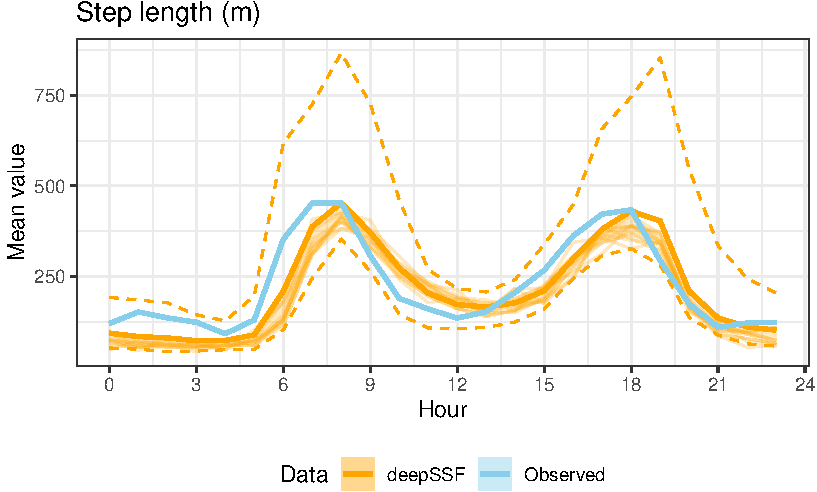
\includegraphics[keepaspectratio]{deepSSF_assessing_trajectories_files/figure-pdf/unnamed-chunk-23-1.pdf}}

\subsection{NDVI}

\begin{Shaded}
\begin{Highlighting}[]
\NormalTok{hourly\_path\_ndvi\_plot }\OtherTok{\textless{}{-}} \FunctionTok{ggplot}\NormalTok{() }\SpecialCharTok{+}
  
  \FunctionTok{geom\_ribbon}\NormalTok{(}\AttributeTok{data =}\NormalTok{ covariate\_summaries\_hourly,}
              \FunctionTok{aes}\NormalTok{(}\AttributeTok{x =}\NormalTok{ hour\_t1, }\AttributeTok{ymin =}\NormalTok{ ndvi\_q25, }\AttributeTok{ymax =}\NormalTok{ ndvi\_q75),}
              \AttributeTok{colour =} \StringTok{"lightgrey"}\NormalTok{, }\AttributeTok{alpha =} \FloatTok{0.15}\NormalTok{) }\SpecialCharTok{+}
  
  \CommentTok{\# geom\_path(data = covariate\_summaries\_hourly,}
  \CommentTok{\#           aes(x = hour\_t1, y = ndvi\_q025),}
  \CommentTok{\#           colour = "black", linetype = "dashed") +}
  \CommentTok{\# }
  \CommentTok{\# geom\_path(data = covariate\_summaries\_hourly,}
  \CommentTok{\#           aes(x = hour\_t1, y = ndvi\_q975),}
  \CommentTok{\#           colour = "black", linetype = "dashed") +}

  \FunctionTok{geom\_path}\NormalTok{(}\AttributeTok{data =}\NormalTok{ covariate\_summaries\_hourly,}
            \FunctionTok{aes}\NormalTok{(}\AttributeTok{x =}\NormalTok{ hour\_t1, }\AttributeTok{y =}\NormalTok{ ndvi\_mean),}
            \AttributeTok{colour =} \StringTok{"black"}\NormalTok{, }\AttributeTok{linetype =} \StringTok{"dashed"}\NormalTok{) }\SpecialCharTok{+}

  \FunctionTok{geom\_ribbon}\NormalTok{(}\AttributeTok{data =}\NormalTok{ hourly\_summary\_quantiles }\SpecialCharTok{\%\textgreater{}\%} 
                \FunctionTok{filter}\NormalTok{(Data }\SpecialCharTok{==} \StringTok{"Buffalo"} \SpecialCharTok{\&}\NormalTok{ variable }\SpecialCharTok{==} \StringTok{"ndvi\_mean"}\NormalTok{),}
              \FunctionTok{aes}\NormalTok{(}\AttributeTok{x =}\NormalTok{ hour\_t1, }\AttributeTok{ymin =}\NormalTok{ q25, }\AttributeTok{ymax =}\NormalTok{ q75, }\AttributeTok{fill =}\NormalTok{ Data),}
              \AttributeTok{alpha =}\NormalTok{ ribbon\_50\_alpha) }\SpecialCharTok{+}

  \FunctionTok{geom\_ribbon}\NormalTok{(}\AttributeTok{data =}\NormalTok{ hourly\_summary\_quantiles }\SpecialCharTok{\%\textgreater{}\%} 
                \FunctionTok{filter}\NormalTok{(}\SpecialCharTok{!}\NormalTok{Data }\SpecialCharTok{==} \StringTok{"Buffalo"} \SpecialCharTok{\&}\NormalTok{ variable }\SpecialCharTok{==} \StringTok{"ndvi\_mean"}\NormalTok{),}
              \FunctionTok{aes}\NormalTok{(}\AttributeTok{x =}\NormalTok{ hour\_t1, }\AttributeTok{ymin =}\NormalTok{ q25, }\AttributeTok{ymax =}\NormalTok{ q75, }\AttributeTok{fill =}\NormalTok{ Data),}
              \AttributeTok{alpha =}\NormalTok{ ribbon\_50\_alpha) }\SpecialCharTok{+}
  
  
  \FunctionTok{geom\_path}\NormalTok{(}\AttributeTok{data =}\NormalTok{ hourly\_habitat\_long }\SpecialCharTok{\%\textgreater{}\%} \FunctionTok{filter}\NormalTok{(id }\SpecialCharTok{\textless{}} \DecValTok{10}\NormalTok{) }\SpecialCharTok{\%\textgreater{}\%} 
              \FunctionTok{filter}\NormalTok{(}\SpecialCharTok{!}\NormalTok{Data }\SpecialCharTok{==} \StringTok{"Buffalo"} \SpecialCharTok{\&}\NormalTok{ variable }\SpecialCharTok{==} \StringTok{"ndvi\_mean"}\NormalTok{),}
                 \FunctionTok{aes}\NormalTok{(}\AttributeTok{x =}\NormalTok{ hour\_t1, }\AttributeTok{y =}\NormalTok{ value, }\AttributeTok{colour =}\NormalTok{ Data, }\AttributeTok{group =} \FunctionTok{interaction}\NormalTok{(id, Data)),}
                 \AttributeTok{alpha =}\NormalTok{ buff\_path\_alpha,}
              \AttributeTok{linewidth =}\NormalTok{ buff\_path\_linewidth) }\SpecialCharTok{+}
  
  
  \FunctionTok{geom\_path}\NormalTok{(}\AttributeTok{data =}\NormalTok{ hourly\_habitat\_long }\SpecialCharTok{\%\textgreater{}\%} 
              \FunctionTok{filter}\NormalTok{(Data }\SpecialCharTok{==} \StringTok{"Buffalo"} \SpecialCharTok{\&}\NormalTok{ variable }\SpecialCharTok{==} \StringTok{"ndvi\_mean"}\NormalTok{),}
                 \FunctionTok{aes}\NormalTok{(}\AttributeTok{x =}\NormalTok{ hour\_t1, }\AttributeTok{y =}\NormalTok{ value, }\AttributeTok{colour =}\NormalTok{ Data, }\AttributeTok{group =} \FunctionTok{interaction}\NormalTok{(id, Data)),}
                 \AttributeTok{alpha =}\NormalTok{ buff\_path\_alpha,}
              \AttributeTok{linewidth =}\NormalTok{ buff\_path\_linewidth) }\SpecialCharTok{+}

  \FunctionTok{geom\_path}\NormalTok{(}\AttributeTok{data =}\NormalTok{ hourly\_summary\_quantiles }\SpecialCharTok{\%\textgreater{}\%} 
              \FunctionTok{filter}\NormalTok{(}\SpecialCharTok{!}\NormalTok{Data }\SpecialCharTok{==} \StringTok{"Buffalo"} \SpecialCharTok{\&}\NormalTok{ variable }\SpecialCharTok{==} \StringTok{"ndvi\_mean"}\NormalTok{),}
              \FunctionTok{aes}\NormalTok{(}\AttributeTok{x =}\NormalTok{ hour\_t1, }\AttributeTok{y =}\NormalTok{ q025, }\AttributeTok{colour =}\NormalTok{ Data),}
            \AttributeTok{linetype =} \StringTok{"dashed"}\NormalTok{,}
              \AttributeTok{alpha =}\NormalTok{ path\_95\_alpha) }\SpecialCharTok{+}

  \FunctionTok{geom\_path}\NormalTok{(}\AttributeTok{data =}\NormalTok{ hourly\_summary\_quantiles }\SpecialCharTok{\%\textgreater{}\%} 
              \FunctionTok{filter}\NormalTok{(}\SpecialCharTok{!}\NormalTok{Data }\SpecialCharTok{==} \StringTok{"Buffalo"} \SpecialCharTok{\&}\NormalTok{ variable }\SpecialCharTok{==} \StringTok{"ndvi\_mean"}\NormalTok{),}
              \FunctionTok{aes}\NormalTok{(}\AttributeTok{x =}\NormalTok{ hour\_t1, }\AttributeTok{y =}\NormalTok{ q975, }\AttributeTok{colour =}\NormalTok{ Data),}
            \AttributeTok{linetype =} \StringTok{"dashed"}\NormalTok{,}
              \AttributeTok{alpha =}\NormalTok{ path\_95\_alpha) }\SpecialCharTok{+}
  
  \FunctionTok{geom\_path}\NormalTok{(}\AttributeTok{data =}\NormalTok{ hourly\_summary\_quantiles }\SpecialCharTok{\%\textgreater{}\%} 
              \FunctionTok{filter}\NormalTok{(Data }\SpecialCharTok{==} \StringTok{"Buffalo"} \SpecialCharTok{\&}\NormalTok{ variable }\SpecialCharTok{==} \StringTok{"ndvi\_mean"}\NormalTok{),}
              \FunctionTok{aes}\NormalTok{(}\AttributeTok{x =}\NormalTok{ hour\_t1, }\AttributeTok{y =}\NormalTok{ mean, }\AttributeTok{colour =}\NormalTok{ Data),}
              \AttributeTok{linewidth =} \DecValTok{1}\NormalTok{) }\SpecialCharTok{+}
  
  \FunctionTok{geom\_path}\NormalTok{(}\AttributeTok{data =}\NormalTok{ hourly\_summary\_quantiles }\SpecialCharTok{\%\textgreater{}\%} 
              \FunctionTok{filter}\NormalTok{(}\SpecialCharTok{!}\NormalTok{Data }\SpecialCharTok{==} \StringTok{"Buffalo"} \SpecialCharTok{\&}\NormalTok{ variable }\SpecialCharTok{==} \StringTok{"ndvi\_mean"}\NormalTok{),}
              \FunctionTok{aes}\NormalTok{(}\AttributeTok{x =}\NormalTok{ hour\_t1, }\AttributeTok{y =}\NormalTok{ mean, }\AttributeTok{colour =}\NormalTok{ Data),}
              \AttributeTok{linewidth =} \DecValTok{1}\NormalTok{) }\SpecialCharTok{+}
    
  \FunctionTok{scale\_fill\_manual}\NormalTok{(}\AttributeTok{values =}\NormalTok{ colors) }\SpecialCharTok{+}
  \FunctionTok{scale\_colour\_manual}\NormalTok{(}\AttributeTok{values =}\NormalTok{ colors) }\SpecialCharTok{+}
  \FunctionTok{scale\_y\_continuous}\NormalTok{(}\StringTok{"Mean value"}\NormalTok{) }\SpecialCharTok{+}
  \FunctionTok{scale\_x\_continuous}\NormalTok{(}\StringTok{"Hour"}\NormalTok{, }\AttributeTok{breaks =} \FunctionTok{seq}\NormalTok{(}\DecValTok{0}\NormalTok{,}\DecValTok{24}\NormalTok{,}\DecValTok{3}\NormalTok{)) }\SpecialCharTok{+}
  \FunctionTok{ggtitle}\NormalTok{(}\StringTok{"NDVI"}\NormalTok{) }\SpecialCharTok{+}
  \FunctionTok{theme\_bw}\NormalTok{()}

\NormalTok{hourly\_path\_ndvi\_plot}
\end{Highlighting}
\end{Shaded}

\pandocbounded{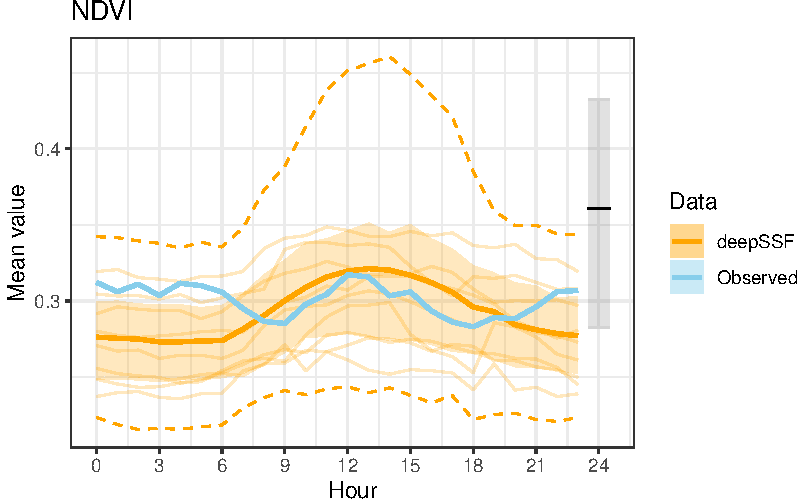
\includegraphics[keepaspectratio]{deepSSF_assessing_trajectories_files/figure-pdf/unnamed-chunk-24-1.pdf}}

\subsection{Canopy cover}

\begin{Shaded}
\begin{Highlighting}[]
\NormalTok{hourly\_path\_canopy\_plot }\OtherTok{\textless{}{-}} \FunctionTok{ggplot}\NormalTok{() }\SpecialCharTok{+}
  
  \FunctionTok{geom\_ribbon}\NormalTok{(}\AttributeTok{data =}\NormalTok{ covariate\_summaries\_hourly,}
              \FunctionTok{aes}\NormalTok{(}\AttributeTok{x =}\NormalTok{ hour\_t1, }\AttributeTok{ymin =}\NormalTok{ canopy\_q25, }\AttributeTok{ymax =}\NormalTok{ canopy\_q75),}
              \AttributeTok{colour =} \StringTok{"lightgrey"}\NormalTok{, }\AttributeTok{alpha =} \FloatTok{0.15}\NormalTok{) }\SpecialCharTok{+}
  
  \CommentTok{\# geom\_path(data = covariate\_summaries\_hourly,}
  \CommentTok{\#           aes(x = hour\_t1, y = canopy\_q025),}
  \CommentTok{\#           colour = "grey", linetype = "dashed") +}
  \CommentTok{\# }
  \CommentTok{\# geom\_path(data = covariate\_summaries\_hourly,}
  \CommentTok{\#           aes(x = hour\_t1, y = canopy\_q975),}
  \CommentTok{\#           colour = "grey", linetype = "dashed") +}

  \FunctionTok{geom\_path}\NormalTok{(}\AttributeTok{data =}\NormalTok{ covariate\_summaries\_hourly,}
            \FunctionTok{aes}\NormalTok{(}\AttributeTok{x =}\NormalTok{ hour\_t1, }\AttributeTok{y =}\NormalTok{ canopy\_mean),}
            \AttributeTok{colour =} \StringTok{"black"}\NormalTok{, }\AttributeTok{linetype =} \StringTok{"dashed"}\NormalTok{) }\SpecialCharTok{+}

  \FunctionTok{geom\_ribbon}\NormalTok{(}\AttributeTok{data =}\NormalTok{ hourly\_summary\_quantiles }\SpecialCharTok{\%\textgreater{}\%} 
                \FunctionTok{filter}\NormalTok{(Data }\SpecialCharTok{==} \StringTok{"Buffalo"} \SpecialCharTok{\&}\NormalTok{ variable }\SpecialCharTok{==} \StringTok{"canopy\_mean"}\NormalTok{),}
              \FunctionTok{aes}\NormalTok{(}\AttributeTok{x =}\NormalTok{ hour\_t1, }\AttributeTok{ymin =}\NormalTok{ q25, }\AttributeTok{ymax =}\NormalTok{ q75, }\AttributeTok{fill =}\NormalTok{ Data),}
              \AttributeTok{alpha =}\NormalTok{ ribbon\_50\_alpha) }\SpecialCharTok{+}

  \FunctionTok{geom\_ribbon}\NormalTok{(}\AttributeTok{data =}\NormalTok{ hourly\_summary\_quantiles }\SpecialCharTok{\%\textgreater{}\%} 
                \FunctionTok{filter}\NormalTok{(}\SpecialCharTok{!}\NormalTok{Data }\SpecialCharTok{==} \StringTok{"Buffalo"} \SpecialCharTok{\&}\NormalTok{ variable }\SpecialCharTok{==} \StringTok{"canopy\_mean"}\NormalTok{),}
              \FunctionTok{aes}\NormalTok{(}\AttributeTok{x =}\NormalTok{ hour\_t1, }\AttributeTok{ymin =}\NormalTok{ q25, }\AttributeTok{ymax =}\NormalTok{ q75, }\AttributeTok{fill =}\NormalTok{ Data),}
              \AttributeTok{alpha =}\NormalTok{ ribbon\_50\_alpha) }\SpecialCharTok{+}
  
  \FunctionTok{geom\_path}\NormalTok{(}\AttributeTok{data =}\NormalTok{ hourly\_habitat\_long }\SpecialCharTok{\%\textgreater{}\%} \FunctionTok{filter}\NormalTok{(id }\SpecialCharTok{\textless{}} \DecValTok{10}\NormalTok{) }\SpecialCharTok{\%\textgreater{}\%} 
              \FunctionTok{filter}\NormalTok{(}\SpecialCharTok{!}\NormalTok{Data }\SpecialCharTok{==} \StringTok{"Buffalo"} \SpecialCharTok{\&}\NormalTok{ variable }\SpecialCharTok{==} \StringTok{"canopy\_mean"}\NormalTok{),}
                 \FunctionTok{aes}\NormalTok{(}\AttributeTok{x =}\NormalTok{ hour\_t1, }\AttributeTok{y =}\NormalTok{ value, }\AttributeTok{colour =}\NormalTok{ Data, }\AttributeTok{group =} \FunctionTok{interaction}\NormalTok{(id, Data)),}
                 \AttributeTok{alpha =}\NormalTok{ buff\_path\_alpha,}
              \AttributeTok{linewidth =}\NormalTok{ buff\_path\_linewidth) }\SpecialCharTok{+}
  
  \FunctionTok{geom\_path}\NormalTok{(}\AttributeTok{data =}\NormalTok{ hourly\_habitat\_long }\SpecialCharTok{\%\textgreater{}\%} 
              \FunctionTok{filter}\NormalTok{(Data }\SpecialCharTok{==} \StringTok{"Buffalo"} \SpecialCharTok{\&}\NormalTok{ variable }\SpecialCharTok{==} \StringTok{"canopy\_mean"}\NormalTok{), }
                 \FunctionTok{aes}\NormalTok{(}\AttributeTok{x =}\NormalTok{ hour\_t1, }\AttributeTok{y =}\NormalTok{ value, }\AttributeTok{colour =}\NormalTok{ Data, }\AttributeTok{group =} \FunctionTok{interaction}\NormalTok{(id, Data)), }
                 \AttributeTok{alpha =}\NormalTok{ buff\_path\_alpha,}
              \AttributeTok{linewidth =}\NormalTok{ buff\_path\_linewidth) }\SpecialCharTok{+}

  \FunctionTok{geom\_path}\NormalTok{(}\AttributeTok{data =}\NormalTok{ hourly\_summary\_quantiles }\SpecialCharTok{\%\textgreater{}\%} 
              \FunctionTok{filter}\NormalTok{(}\SpecialCharTok{!}\NormalTok{Data }\SpecialCharTok{==} \StringTok{"Buffalo"} \SpecialCharTok{\&}\NormalTok{ variable }\SpecialCharTok{==} \StringTok{"canopy\_mean"}\NormalTok{),}
              \FunctionTok{aes}\NormalTok{(}\AttributeTok{x =}\NormalTok{ hour\_t1, }\AttributeTok{y =}\NormalTok{ q025, }\AttributeTok{colour =}\NormalTok{ Data),}
            \AttributeTok{linetype =} \StringTok{"dashed"}\NormalTok{,}
              \AttributeTok{alpha =}\NormalTok{ path\_95\_alpha) }\SpecialCharTok{+}

  \FunctionTok{geom\_path}\NormalTok{(}\AttributeTok{data =}\NormalTok{ hourly\_summary\_quantiles }\SpecialCharTok{\%\textgreater{}\%} 
              \FunctionTok{filter}\NormalTok{(}\SpecialCharTok{!}\NormalTok{Data }\SpecialCharTok{==} \StringTok{"Buffalo"} \SpecialCharTok{\&}\NormalTok{ variable }\SpecialCharTok{==} \StringTok{"canopy\_mean"}\NormalTok{),}
              \FunctionTok{aes}\NormalTok{(}\AttributeTok{x =}\NormalTok{ hour\_t1, }\AttributeTok{y =}\NormalTok{ q975, }\AttributeTok{colour =}\NormalTok{ Data),}
            \AttributeTok{linetype =} \StringTok{"dashed"}\NormalTok{,}
              \AttributeTok{alpha =}\NormalTok{ path\_95\_alpha) }\SpecialCharTok{+}
  
  \FunctionTok{geom\_path}\NormalTok{(}\AttributeTok{data =}\NormalTok{ hourly\_summary\_quantiles }\SpecialCharTok{\%\textgreater{}\%} 
              \FunctionTok{filter}\NormalTok{(Data }\SpecialCharTok{==} \StringTok{"Buffalo"} \SpecialCharTok{\&}\NormalTok{ variable }\SpecialCharTok{==} \StringTok{"canopy\_mean"}\NormalTok{),}
              \FunctionTok{aes}\NormalTok{(}\AttributeTok{x =}\NormalTok{ hour\_t1, }\AttributeTok{y =}\NormalTok{ mean, }\AttributeTok{colour =}\NormalTok{ Data),}
              \AttributeTok{linewidth =} \DecValTok{1}\NormalTok{) }\SpecialCharTok{+}
  
  \FunctionTok{geom\_path}\NormalTok{(}\AttributeTok{data =}\NormalTok{ hourly\_summary\_quantiles }\SpecialCharTok{\%\textgreater{}\%} 
              \FunctionTok{filter}\NormalTok{(}\SpecialCharTok{!}\NormalTok{Data }\SpecialCharTok{==} \StringTok{"Buffalo"} \SpecialCharTok{\&}\NormalTok{ variable }\SpecialCharTok{==} \StringTok{"canopy\_mean"}\NormalTok{),}
              \FunctionTok{aes}\NormalTok{(}\AttributeTok{x =}\NormalTok{ hour\_t1, }\AttributeTok{y =}\NormalTok{ mean, }\AttributeTok{colour =}\NormalTok{ Data),}
              \AttributeTok{linewidth =} \DecValTok{1}\NormalTok{) }\SpecialCharTok{+}
    
  \FunctionTok{scale\_fill\_manual}\NormalTok{(}\AttributeTok{values =}\NormalTok{ colors) }\SpecialCharTok{+} 
  \FunctionTok{scale\_colour\_manual}\NormalTok{(}\AttributeTok{values =}\NormalTok{ colors) }\SpecialCharTok{+}
  \FunctionTok{scale\_y\_continuous}\NormalTok{(}\StringTok{"Mean value"}\NormalTok{) }\SpecialCharTok{+}
  \FunctionTok{scale\_x\_continuous}\NormalTok{(}\StringTok{"Hour"}\NormalTok{, }\AttributeTok{breaks =} \FunctionTok{seq}\NormalTok{(}\DecValTok{0}\NormalTok{,}\DecValTok{24}\NormalTok{,}\DecValTok{3}\NormalTok{)) }\SpecialCharTok{+}
  \FunctionTok{ggtitle}\NormalTok{(}\StringTok{"Canopy cover"}\NormalTok{) }\SpecialCharTok{+}
  \FunctionTok{theme\_bw}\NormalTok{()}

\NormalTok{hourly\_path\_canopy\_plot}
\end{Highlighting}
\end{Shaded}

\pandocbounded{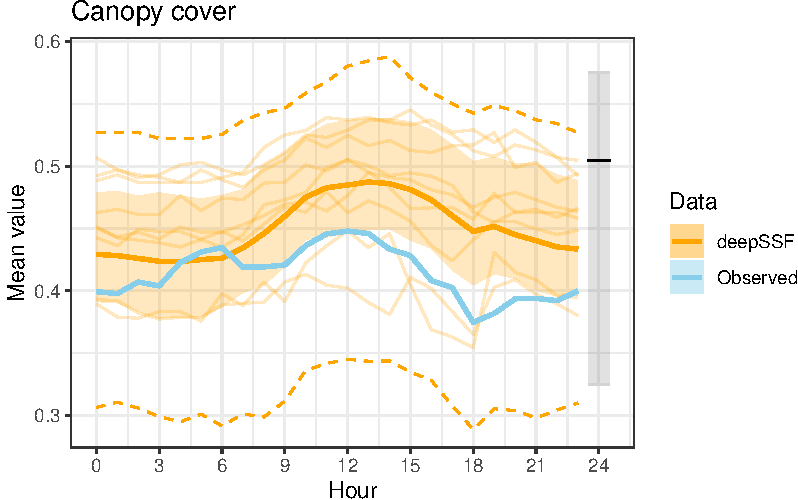
\includegraphics[keepaspectratio]{deepSSF_assessing_trajectories_files/figure-pdf/unnamed-chunk-25-1.pdf}}

\subsection{Herbaceous vegetation}

\begin{Shaded}
\begin{Highlighting}[]
\NormalTok{hourly\_path\_herby\_plot }\OtherTok{\textless{}{-}} \FunctionTok{ggplot}\NormalTok{() }\SpecialCharTok{+}
  
  \FunctionTok{geom\_ribbon}\NormalTok{(}\AttributeTok{data =}\NormalTok{ covariate\_summaries\_hourly,}
              \FunctionTok{aes}\NormalTok{(}\AttributeTok{x =}\NormalTok{ hour\_t1, }\AttributeTok{ymin =}\NormalTok{ veg\_herby\_q25, }\AttributeTok{ymax =}\NormalTok{ veg\_herby\_q75),}
              \AttributeTok{colour =} \StringTok{"lightgrey"}\NormalTok{, }\AttributeTok{alpha =} \FloatTok{0.15}\NormalTok{) }\SpecialCharTok{+}
  
  \CommentTok{\# geom\_path(data = covariate\_summaries\_hourly,}
  \CommentTok{\#           aes(x = hour\_t1, y = veg\_herby\_q025),}
  \CommentTok{\#           colour = "grey", linetype = "dashed") +}
  \CommentTok{\# }
  \CommentTok{\# geom\_path(data = covariate\_summaries\_hourly,}
  \CommentTok{\#           aes(x = hour\_t1, y = veg\_herby\_q975),}
  \CommentTok{\#           colour = "grey", linetype = "dashed") +}

  \FunctionTok{geom\_path}\NormalTok{(}\AttributeTok{data =}\NormalTok{ covariate\_summaries\_hourly,}
            \FunctionTok{aes}\NormalTok{(}\AttributeTok{x =}\NormalTok{ hour\_t1, }\AttributeTok{y =}\NormalTok{ veg\_herby\_mean),}
            \AttributeTok{colour =} \StringTok{"black"}\NormalTok{, }\AttributeTok{linetype =} \StringTok{"dashed"}\NormalTok{) }\SpecialCharTok{+}

  \FunctionTok{geom\_ribbon}\NormalTok{(}\AttributeTok{data =}\NormalTok{ hourly\_summary\_quantiles }\SpecialCharTok{\%\textgreater{}\%} 
                \FunctionTok{filter}\NormalTok{(Data }\SpecialCharTok{==} \StringTok{"Buffalo"} \SpecialCharTok{\&}\NormalTok{ variable }\SpecialCharTok{==} \StringTok{"herby\_mean"}\NormalTok{),}
              \FunctionTok{aes}\NormalTok{(}\AttributeTok{x =}\NormalTok{ hour\_t1, }\AttributeTok{ymin =}\NormalTok{ q25, }\AttributeTok{ymax =}\NormalTok{ q75, }\AttributeTok{fill =}\NormalTok{ Data),}
              \AttributeTok{alpha =}\NormalTok{ ribbon\_50\_alpha) }\SpecialCharTok{+}

  \FunctionTok{geom\_ribbon}\NormalTok{(}\AttributeTok{data =}\NormalTok{ hourly\_summary\_quantiles }\SpecialCharTok{\%\textgreater{}\%} 
                \FunctionTok{filter}\NormalTok{(}\SpecialCharTok{!}\NormalTok{Data }\SpecialCharTok{==} \StringTok{"Buffalo"} \SpecialCharTok{\&}\NormalTok{ variable }\SpecialCharTok{==} \StringTok{"herby\_mean"}\NormalTok{),}
              \FunctionTok{aes}\NormalTok{(}\AttributeTok{x =}\NormalTok{ hour\_t1, }\AttributeTok{ymin =}\NormalTok{ q25, }\AttributeTok{ymax =}\NormalTok{ q75, }\AttributeTok{fill =}\NormalTok{ Data),}
              \AttributeTok{alpha =}\NormalTok{ ribbon\_50\_alpha) }\SpecialCharTok{+}
  
  \FunctionTok{geom\_path}\NormalTok{(}\AttributeTok{data =}\NormalTok{ hourly\_habitat\_long }\SpecialCharTok{\%\textgreater{}\%} \FunctionTok{filter}\NormalTok{(id }\SpecialCharTok{\textless{}} \DecValTok{10}\NormalTok{) }\SpecialCharTok{\%\textgreater{}\%} 
              \FunctionTok{filter}\NormalTok{(}\SpecialCharTok{!}\NormalTok{Data }\SpecialCharTok{==} \StringTok{"Buffalo"} \SpecialCharTok{\&}\NormalTok{ variable }\SpecialCharTok{==} \StringTok{"herby\_mean"}\NormalTok{),}
                 \FunctionTok{aes}\NormalTok{(}\AttributeTok{x =}\NormalTok{ hour\_t1, }\AttributeTok{y =}\NormalTok{ value, }\AttributeTok{colour =}\NormalTok{ Data, }\AttributeTok{group =} \FunctionTok{interaction}\NormalTok{(id, Data)),}
                 \AttributeTok{alpha =}\NormalTok{ buff\_path\_alpha,}
              \AttributeTok{linewidth =}\NormalTok{ buff\_path\_linewidth) }\SpecialCharTok{+}
  
  \FunctionTok{geom\_path}\NormalTok{(}\AttributeTok{data =}\NormalTok{ hourly\_habitat\_long }\SpecialCharTok{\%\textgreater{}\%} 
              \FunctionTok{filter}\NormalTok{(Data }\SpecialCharTok{==} \StringTok{"Buffalo"} \SpecialCharTok{\&}\NormalTok{ variable }\SpecialCharTok{==} \StringTok{"herby\_mean"}\NormalTok{), }
                 \FunctionTok{aes}\NormalTok{(}\AttributeTok{x =}\NormalTok{ hour\_t1, }\AttributeTok{y =}\NormalTok{ value, }\AttributeTok{colour =}\NormalTok{ Data, }\AttributeTok{group =} \FunctionTok{interaction}\NormalTok{(id, Data)), }
                 \AttributeTok{alpha =}\NormalTok{ buff\_path\_alpha,}
              \AttributeTok{linewidth =}\NormalTok{ buff\_path\_linewidth) }\SpecialCharTok{+}

  \FunctionTok{geom\_path}\NormalTok{(}\AttributeTok{data =}\NormalTok{ hourly\_summary\_quantiles }\SpecialCharTok{\%\textgreater{}\%} 
              \FunctionTok{filter}\NormalTok{(}\SpecialCharTok{!}\NormalTok{Data }\SpecialCharTok{==} \StringTok{"Buffalo"} \SpecialCharTok{\&}\NormalTok{ variable }\SpecialCharTok{==} \StringTok{"herby\_mean"}\NormalTok{),}
              \FunctionTok{aes}\NormalTok{(}\AttributeTok{x =}\NormalTok{ hour\_t1, }\AttributeTok{y =}\NormalTok{ q025, }\AttributeTok{colour =}\NormalTok{ Data),}
            \AttributeTok{linetype =} \StringTok{"dashed"}\NormalTok{,}
              \AttributeTok{alpha =}\NormalTok{ path\_95\_alpha) }\SpecialCharTok{+}

  \FunctionTok{geom\_path}\NormalTok{(}\AttributeTok{data =}\NormalTok{ hourly\_summary\_quantiles }\SpecialCharTok{\%\textgreater{}\%} 
              \FunctionTok{filter}\NormalTok{(}\SpecialCharTok{!}\NormalTok{Data }\SpecialCharTok{==} \StringTok{"Buffalo"} \SpecialCharTok{\&}\NormalTok{ variable }\SpecialCharTok{==} \StringTok{"herby\_mean"}\NormalTok{),}
              \FunctionTok{aes}\NormalTok{(}\AttributeTok{x =}\NormalTok{ hour\_t1, }\AttributeTok{y =}\NormalTok{ q975, }\AttributeTok{colour =}\NormalTok{ Data),}
            \AttributeTok{linetype =} \StringTok{"dashed"}\NormalTok{,}
              \AttributeTok{alpha =}\NormalTok{ path\_95\_alpha) }\SpecialCharTok{+}
  
  \FunctionTok{geom\_path}\NormalTok{(}\AttributeTok{data =}\NormalTok{ hourly\_summary\_quantiles }\SpecialCharTok{\%\textgreater{}\%} 
              \FunctionTok{filter}\NormalTok{(Data }\SpecialCharTok{==} \StringTok{"Buffalo"} \SpecialCharTok{\&}\NormalTok{ variable }\SpecialCharTok{==} \StringTok{"herby\_mean"}\NormalTok{),}
              \FunctionTok{aes}\NormalTok{(}\AttributeTok{x =}\NormalTok{ hour\_t1, }\AttributeTok{y =}\NormalTok{ mean, }\AttributeTok{colour =}\NormalTok{ Data),}
              \AttributeTok{linewidth =} \DecValTok{1}\NormalTok{) }\SpecialCharTok{+}
  
  \FunctionTok{geom\_path}\NormalTok{(}\AttributeTok{data =}\NormalTok{ hourly\_summary\_quantiles }\SpecialCharTok{\%\textgreater{}\%} 
              \FunctionTok{filter}\NormalTok{(}\SpecialCharTok{!}\NormalTok{Data }\SpecialCharTok{==} \StringTok{"Buffalo"} \SpecialCharTok{\&}\NormalTok{ variable }\SpecialCharTok{==} \StringTok{"herby\_mean"}\NormalTok{),}
              \FunctionTok{aes}\NormalTok{(}\AttributeTok{x =}\NormalTok{ hour\_t1, }\AttributeTok{y =}\NormalTok{ mean, }\AttributeTok{colour =}\NormalTok{ Data),}
              \AttributeTok{linewidth =} \DecValTok{1}\NormalTok{) }\SpecialCharTok{+}
    
  \FunctionTok{scale\_fill\_manual}\NormalTok{(}\AttributeTok{values =}\NormalTok{ colors) }\SpecialCharTok{+} 
  \FunctionTok{scale\_colour\_manual}\NormalTok{(}\AttributeTok{values =}\NormalTok{ colors) }\SpecialCharTok{+}
  \FunctionTok{scale\_y\_continuous}\NormalTok{(}\StringTok{"Mean value"}\NormalTok{) }\SpecialCharTok{+}
  \FunctionTok{scale\_x\_continuous}\NormalTok{(}\StringTok{"Hour"}\NormalTok{, }\AttributeTok{breaks =} \FunctionTok{seq}\NormalTok{(}\DecValTok{0}\NormalTok{,}\DecValTok{24}\NormalTok{,}\DecValTok{3}\NormalTok{)) }\SpecialCharTok{+}
  \FunctionTok{ggtitle}\NormalTok{(}\StringTok{"Herbaceous vegetation"}\NormalTok{) }\SpecialCharTok{+}
  \FunctionTok{theme\_bw}\NormalTok{()}

\NormalTok{hourly\_path\_herby\_plot}
\end{Highlighting}
\end{Shaded}

\pandocbounded{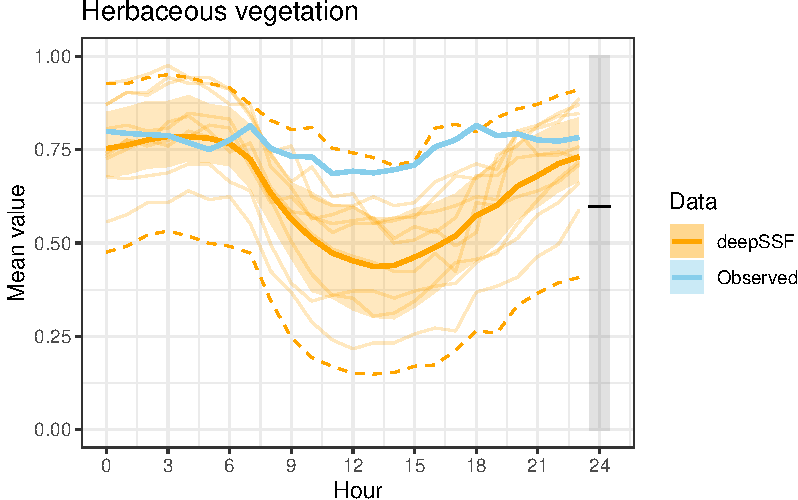
\includegraphics[keepaspectratio]{deepSSF_assessing_trajectories_files/figure-pdf/unnamed-chunk-26-1.pdf}}

\subsection{Slope}

\begin{Shaded}
\begin{Highlighting}[]
\NormalTok{hourly\_path\_slope\_plot }\OtherTok{\textless{}{-}} \FunctionTok{ggplot}\NormalTok{() }\SpecialCharTok{+}
  
  \FunctionTok{geom\_ribbon}\NormalTok{(}\AttributeTok{data =}\NormalTok{ covariate\_summaries\_hourly,}
              \FunctionTok{aes}\NormalTok{(}\AttributeTok{x =}\NormalTok{ hour\_t1, }\AttributeTok{ymin =}\NormalTok{ slope\_q25, }\AttributeTok{ymax =}\NormalTok{ slope\_q75),}
              \AttributeTok{colour =} \StringTok{"lightgrey"}\NormalTok{, }\AttributeTok{alpha =} \FloatTok{0.15}\NormalTok{) }\SpecialCharTok{+}
  
  \CommentTok{\# geom\_path(data = covariate\_summaries\_hourly,}
  \CommentTok{\#           aes(x = hour\_t1, y = slope\_q025),}
  \CommentTok{\#           colour = "grey", linetype = "dashed") +}
  \CommentTok{\# }
  \CommentTok{\# geom\_path(data = covariate\_summaries\_hourly,}
  \CommentTok{\#           aes(x = hour\_t1, y = slope\_q975),}
  \CommentTok{\#           colour = "grey", linetype = "dashed") +}

  \FunctionTok{geom\_path}\NormalTok{(}\AttributeTok{data =}\NormalTok{ covariate\_summaries\_hourly,}
            \FunctionTok{aes}\NormalTok{(}\AttributeTok{x =}\NormalTok{ hour\_t1, }\AttributeTok{y =}\NormalTok{ slope\_mean),}
            \AttributeTok{colour =} \StringTok{"black"}\NormalTok{, }\AttributeTok{linetype =} \StringTok{"dashed"}\NormalTok{) }\SpecialCharTok{+}

  \FunctionTok{geom\_ribbon}\NormalTok{(}\AttributeTok{data =}\NormalTok{ hourly\_summary\_quantiles }\SpecialCharTok{\%\textgreater{}\%} 
                \FunctionTok{filter}\NormalTok{(Data }\SpecialCharTok{==} \StringTok{"Buffalo"} \SpecialCharTok{\&}\NormalTok{ variable }\SpecialCharTok{==} \StringTok{"slope\_mean"}\NormalTok{),}
              \FunctionTok{aes}\NormalTok{(}\AttributeTok{x =}\NormalTok{ hour\_t1, }\AttributeTok{ymin =}\NormalTok{ q25, }\AttributeTok{ymax =}\NormalTok{ q75, }\AttributeTok{fill =}\NormalTok{ Data),}
              \AttributeTok{alpha =}\NormalTok{ ribbon\_50\_alpha) }\SpecialCharTok{+}

  \FunctionTok{geom\_ribbon}\NormalTok{(}\AttributeTok{data =}\NormalTok{ hourly\_summary\_quantiles }\SpecialCharTok{\%\textgreater{}\%} 
                \FunctionTok{filter}\NormalTok{(}\SpecialCharTok{!}\NormalTok{Data }\SpecialCharTok{==} \StringTok{"Buffalo"} \SpecialCharTok{\&}\NormalTok{ variable }\SpecialCharTok{==} \StringTok{"slope\_mean"}\NormalTok{),}
              \FunctionTok{aes}\NormalTok{(}\AttributeTok{x =}\NormalTok{ hour\_t1, }\AttributeTok{ymin =}\NormalTok{ q25, }\AttributeTok{ymax =}\NormalTok{ q75, }\AttributeTok{fill =}\NormalTok{ Data),}
              \AttributeTok{alpha =}\NormalTok{ ribbon\_50\_alpha) }\SpecialCharTok{+}
  
  \FunctionTok{geom\_path}\NormalTok{(}\AttributeTok{data =}\NormalTok{ hourly\_habitat\_long }\SpecialCharTok{\%\textgreater{}\%} \FunctionTok{filter}\NormalTok{(id }\SpecialCharTok{\textless{}} \DecValTok{10}\NormalTok{) }\SpecialCharTok{\%\textgreater{}\%} 
              \FunctionTok{filter}\NormalTok{(}\SpecialCharTok{!}\NormalTok{Data }\SpecialCharTok{==} \StringTok{"Buffalo"} \SpecialCharTok{\&}\NormalTok{ variable }\SpecialCharTok{==} \StringTok{"slope\_mean"}\NormalTok{),}
                 \FunctionTok{aes}\NormalTok{(}\AttributeTok{x =}\NormalTok{ hour\_t1, }\AttributeTok{y =}\NormalTok{ value, }\AttributeTok{colour =}\NormalTok{ Data, }\AttributeTok{group =} \FunctionTok{interaction}\NormalTok{(id, Data)),}
                 \AttributeTok{alpha =}\NormalTok{ buff\_path\_alpha,}
              \AttributeTok{linewidth =}\NormalTok{ buff\_path\_linewidth) }\SpecialCharTok{+}
  
  \FunctionTok{geom\_path}\NormalTok{(}\AttributeTok{data =}\NormalTok{ hourly\_habitat\_long }\SpecialCharTok{\%\textgreater{}\%} 
              \FunctionTok{filter}\NormalTok{(Data }\SpecialCharTok{==} \StringTok{"Buffalo"} \SpecialCharTok{\&}\NormalTok{ variable }\SpecialCharTok{==} \StringTok{"slope\_mean"}\NormalTok{), }
                 \FunctionTok{aes}\NormalTok{(}\AttributeTok{x =}\NormalTok{ hour\_t1, }\AttributeTok{y =}\NormalTok{ value, }\AttributeTok{colour =}\NormalTok{ Data, }\AttributeTok{group =} \FunctionTok{interaction}\NormalTok{(id, Data)), }
                 \AttributeTok{alpha =}\NormalTok{ buff\_path\_alpha,}
              \AttributeTok{linewidth =}\NormalTok{ buff\_path\_linewidth) }\SpecialCharTok{+}

  \FunctionTok{geom\_path}\NormalTok{(}\AttributeTok{data =}\NormalTok{ hourly\_summary\_quantiles }\SpecialCharTok{\%\textgreater{}\%} 
              \FunctionTok{filter}\NormalTok{(}\SpecialCharTok{!}\NormalTok{Data }\SpecialCharTok{==} \StringTok{"Buffalo"} \SpecialCharTok{\&}\NormalTok{ variable }\SpecialCharTok{==} \StringTok{"slope\_mean"}\NormalTok{),}
              \FunctionTok{aes}\NormalTok{(}\AttributeTok{x =}\NormalTok{ hour\_t1, }\AttributeTok{y =}\NormalTok{ q025, }\AttributeTok{colour =}\NormalTok{ Data),}
            \AttributeTok{linetype =} \StringTok{"dashed"}\NormalTok{,}
              \AttributeTok{alpha =}\NormalTok{ path\_95\_alpha) }\SpecialCharTok{+}

  \FunctionTok{geom\_path}\NormalTok{(}\AttributeTok{data =}\NormalTok{ hourly\_summary\_quantiles }\SpecialCharTok{\%\textgreater{}\%} 
              \FunctionTok{filter}\NormalTok{(}\SpecialCharTok{!}\NormalTok{Data }\SpecialCharTok{==} \StringTok{"Buffalo"} \SpecialCharTok{\&}\NormalTok{ variable }\SpecialCharTok{==} \StringTok{"slope\_mean"}\NormalTok{),}
              \FunctionTok{aes}\NormalTok{(}\AttributeTok{x =}\NormalTok{ hour\_t1, }\AttributeTok{y =}\NormalTok{ q975, }\AttributeTok{colour =}\NormalTok{ Data),}
            \AttributeTok{linetype =} \StringTok{"dashed"}\NormalTok{,}
              \AttributeTok{alpha =}\NormalTok{ path\_95\_alpha) }\SpecialCharTok{+}
  
  \FunctionTok{geom\_path}\NormalTok{(}\AttributeTok{data =}\NormalTok{ hourly\_summary\_quantiles }\SpecialCharTok{\%\textgreater{}\%} 
              \FunctionTok{filter}\NormalTok{(Data }\SpecialCharTok{==} \StringTok{"Buffalo"} \SpecialCharTok{\&}\NormalTok{ variable }\SpecialCharTok{==} \StringTok{"slope\_mean"}\NormalTok{),}
              \FunctionTok{aes}\NormalTok{(}\AttributeTok{x =}\NormalTok{ hour\_t1, }\AttributeTok{y =}\NormalTok{ mean, }\AttributeTok{colour =}\NormalTok{ Data),}
              \AttributeTok{linewidth =} \DecValTok{1}\NormalTok{) }\SpecialCharTok{+}
  
  \FunctionTok{geom\_path}\NormalTok{(}\AttributeTok{data =}\NormalTok{ hourly\_summary\_quantiles }\SpecialCharTok{\%\textgreater{}\%}
              \FunctionTok{filter}\NormalTok{(}\SpecialCharTok{!}\NormalTok{Data }\SpecialCharTok{==} \StringTok{"Buffalo"} \SpecialCharTok{\&}\NormalTok{ variable }\SpecialCharTok{==} \StringTok{"slope\_mean"}\NormalTok{),}
              \FunctionTok{aes}\NormalTok{(}\AttributeTok{x =}\NormalTok{ hour\_t1, }\AttributeTok{y =}\NormalTok{ mean, }\AttributeTok{colour =}\NormalTok{ Data),}
              \AttributeTok{linewidth =} \DecValTok{1}\NormalTok{) }\SpecialCharTok{+}
    
  \FunctionTok{scale\_fill\_manual}\NormalTok{(}\AttributeTok{values =}\NormalTok{ colors) }\SpecialCharTok{+} 
  \FunctionTok{scale\_colour\_manual}\NormalTok{(}\AttributeTok{values =}\NormalTok{ colors) }\SpecialCharTok{+}
  \FunctionTok{scale\_y\_continuous}\NormalTok{(}\StringTok{"Mean value"}\NormalTok{) }\SpecialCharTok{+}
  \FunctionTok{scale\_x\_continuous}\NormalTok{(}\StringTok{"Hour"}\NormalTok{, }\AttributeTok{breaks =} \FunctionTok{seq}\NormalTok{(}\DecValTok{0}\NormalTok{,}\DecValTok{24}\NormalTok{,}\DecValTok{3}\NormalTok{)) }\SpecialCharTok{+}
  \FunctionTok{ggtitle}\NormalTok{(}\StringTok{"Slope"}\NormalTok{) }\SpecialCharTok{+}
  \FunctionTok{theme\_bw}\NormalTok{()}

\NormalTok{hourly\_path\_slope\_plot}
\end{Highlighting}
\end{Shaded}

\pandocbounded{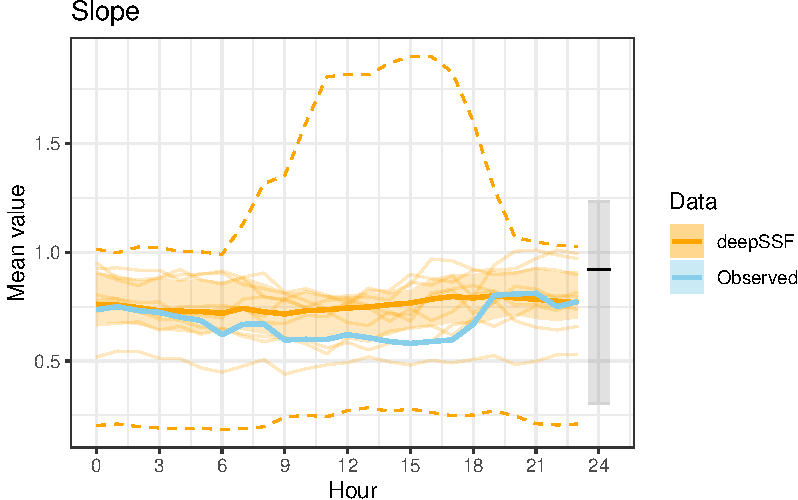
\includegraphics[keepaspectratio]{deepSSF_assessing_trajectories_files/figure-pdf/unnamed-chunk-27-1.pdf}}

\subsection{Combining the hourly
plots}\label{combining-the-hourly-plots}

\begin{Shaded}
\begin{Highlighting}[]
\FunctionTok{ggarrange}\NormalTok{(step\_lengths\_stationary,}
          
\NormalTok{          step\_lengths\_log,}

          \CommentTok{\# hourly\_path\_herby\_plot,}
          \CommentTok{\# }
          \CommentTok{\# hourly\_path\_canopy\_plot +}
          \CommentTok{\#   theme(axis.title.y = element\_blank()),}

          \AttributeTok{labels =} \FunctionTok{c}\NormalTok{(}\StringTok{"A"}\NormalTok{, }\StringTok{"B"}\NormalTok{),}
          \AttributeTok{ncol =} \DecValTok{1}\NormalTok{, }\AttributeTok{nrow =} \DecValTok{2}\NormalTok{,}
          \AttributeTok{legend =} \StringTok{"bottom"}\NormalTok{,}
          \AttributeTok{common.legend =} \ConstantTok{TRUE}\NormalTok{)}
\end{Highlighting}
\end{Shaded}

\begin{verbatim}
Warning: Removed 147 rows containing non-finite outside the scale range
(`stat_density()`).
\end{verbatim}

\begin{verbatim}
Warning: Removed 3703 rows containing non-finite outside the scale range
(`stat_density()`).
\end{verbatim}

\begin{verbatim}
Warning in scale_x_log10("log Step length (m)"): log-10 transformation
introduced infinite values.
\end{verbatim}

\begin{verbatim}
Warning: Removed 51 rows containing non-finite outside the scale range
(`stat_density()`).
\end{verbatim}

\begin{verbatim}
Warning: Removed 147 rows containing non-finite outside the scale range
(`stat_density()`).
\end{verbatim}

\begin{verbatim}
Warning: Removed 3703 rows containing non-finite outside the scale range
(`stat_density()`).
\end{verbatim}

\begin{verbatim}
Warning in scale_x_log10("log Step length (m)"): log-10 transformation
introduced infinite values.
\end{verbatim}

\begin{verbatim}
Warning: Removed 51 rows containing non-finite outside the scale range
(`stat_density()`).
\end{verbatim}

\pandocbounded{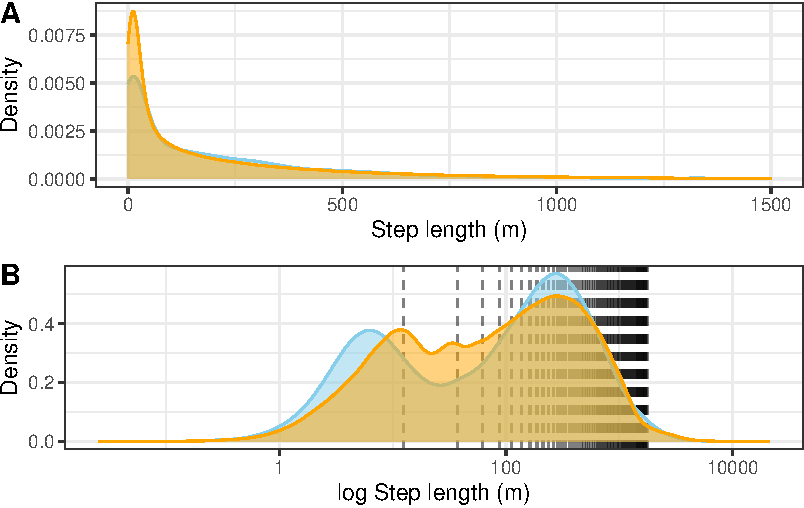
\includegraphics[keepaspectratio]{deepSSF_assessing_trajectories_files/figure-pdf/unnamed-chunk-28-1.pdf}}

\begin{Shaded}
\begin{Highlighting}[]
\FunctionTok{ggsave}\NormalTok{(}\FunctionTok{paste0}\NormalTok{(}\StringTok{"Python/outputs/model\_training/"}\NormalTok{,deepSSF\_dir,}\StringTok{"/step\_lengths\_stat\_log.png"}\NormalTok{), }\AttributeTok{width=}\DecValTok{170}\NormalTok{, }\AttributeTok{height=}\DecValTok{150}\NormalTok{, }\AttributeTok{units=}\StringTok{"mm"}\NormalTok{, }\AttributeTok{dpi =} \DecValTok{600}\NormalTok{)}
\end{Highlighting}
\end{Shaded}

\subsubsection{Step lengths instead of
slope}\label{step-lengths-instead-of-slope}

\begin{Shaded}
\begin{Highlighting}[]
\FunctionTok{ggarrange}\NormalTok{(hourly\_path\_sl\_plot }\SpecialCharTok{+}
            \FunctionTok{theme}\NormalTok{(}\AttributeTok{axis.title.x =} \FunctionTok{element\_blank}\NormalTok{(),}
                  \AttributeTok{axis.text.x =} \FunctionTok{element\_blank}\NormalTok{(),}
                  \AttributeTok{legend.title =} \FunctionTok{element\_blank}\NormalTok{()),}

\NormalTok{          hourly\_path\_ndvi\_plot }\SpecialCharTok{+}
            \FunctionTok{theme}\NormalTok{(}\AttributeTok{axis.title.x =} \FunctionTok{element\_blank}\NormalTok{(),}
                  \AttributeTok{axis.text.x =} \FunctionTok{element\_blank}\NormalTok{(),}
                  \AttributeTok{axis.title.y =} \FunctionTok{element\_blank}\NormalTok{()),}

\NormalTok{          hourly\_path\_herby\_plot,}

\NormalTok{          hourly\_path\_canopy\_plot }\SpecialCharTok{+}
            \FunctionTok{theme}\NormalTok{(}\AttributeTok{axis.title.y =} \FunctionTok{element\_blank}\NormalTok{()),}

          \AttributeTok{labels =} \FunctionTok{c}\NormalTok{(}\StringTok{"A"}\NormalTok{, }\StringTok{"B"}\NormalTok{, }\StringTok{"C"}\NormalTok{, }\StringTok{"D"}\NormalTok{),}
          \AttributeTok{ncol =} \DecValTok{2}\NormalTok{, }\AttributeTok{nrow =} \DecValTok{2}\NormalTok{,}
          \AttributeTok{legend =} \StringTok{"bottom"}\NormalTok{,}
          \AttributeTok{common.legend =} \ConstantTok{TRUE}\NormalTok{)}
\end{Highlighting}
\end{Shaded}

\pandocbounded{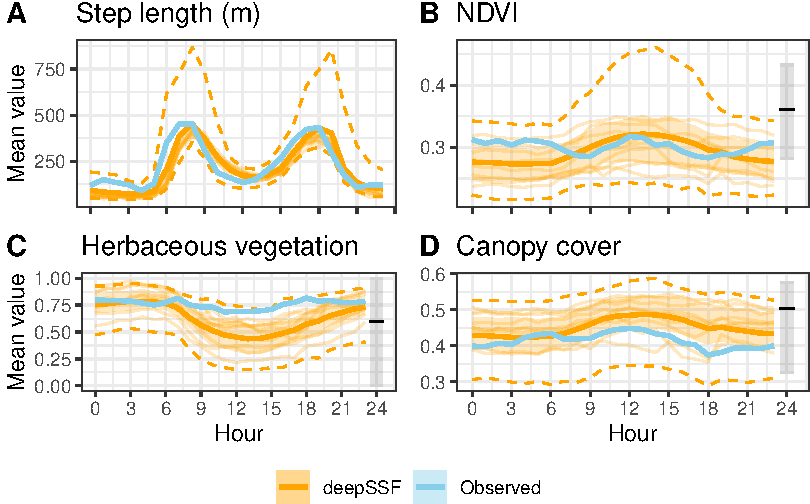
\includegraphics[keepaspectratio]{deepSSF_assessing_trajectories_files/figure-pdf/unnamed-chunk-29-1.pdf}}

\begin{Shaded}
\begin{Highlighting}[]
\FunctionTok{ggsave}\NormalTok{(}\FunctionTok{paste0}\NormalTok{(}\StringTok{"Python/outputs/model\_training/"}\NormalTok{,deepSSF\_dir,}\StringTok{"/hourly\_summaries\_step.png"}\NormalTok{), }\AttributeTok{width=}\DecValTok{180}\NormalTok{, }\AttributeTok{height=}\DecValTok{150}\NormalTok{, }\AttributeTok{units=}\StringTok{"mm"}\NormalTok{, }\AttributeTok{dpi =} \DecValTok{600}\NormalTok{)}
\end{Highlighting}
\end{Shaded}

\subsection{Slope instead of step
lengths}\label{slope-instead-of-step-lengths}

\begin{Shaded}
\begin{Highlighting}[]
\FunctionTok{ggarrange}\NormalTok{(hourly\_path\_ndvi\_plot }\SpecialCharTok{+} 
            \FunctionTok{theme}\NormalTok{(}\AttributeTok{axis.title.x =} \FunctionTok{element\_blank}\NormalTok{(),}
                  \AttributeTok{axis.text.x =} \FunctionTok{element\_blank}\NormalTok{(),}
                  \AttributeTok{legend.title =} \FunctionTok{element\_blank}\NormalTok{()), }
          
\NormalTok{          hourly\_path\_canopy\_plot }\SpecialCharTok{+} 
            \FunctionTok{theme}\NormalTok{(}\AttributeTok{axis.title.x =} \FunctionTok{element\_blank}\NormalTok{(),}
                  \AttributeTok{axis.text.x =} \FunctionTok{element\_blank}\NormalTok{(),}
                  \AttributeTok{axis.title.y =} \FunctionTok{element\_blank}\NormalTok{()), }
          
\NormalTok{          hourly\_path\_herby\_plot, }
          
\NormalTok{          hourly\_path\_slope\_plot }\SpecialCharTok{+}
            \FunctionTok{theme}\NormalTok{(}\AttributeTok{axis.title.y =} \FunctionTok{element\_blank}\NormalTok{()),}
          
          \AttributeTok{labels =} \FunctionTok{c}\NormalTok{(}\StringTok{"A"}\NormalTok{, }\StringTok{"B"}\NormalTok{, }\StringTok{"C"}\NormalTok{, }\StringTok{"D"}\NormalTok{),}
          \AttributeTok{ncol =} \DecValTok{2}\NormalTok{, }\AttributeTok{nrow =} \DecValTok{2}\NormalTok{,}
          \AttributeTok{legend =} \StringTok{"bottom"}\NormalTok{,}
          \AttributeTok{common.legend =} \ConstantTok{TRUE}\NormalTok{)}
\end{Highlighting}
\end{Shaded}

\pandocbounded{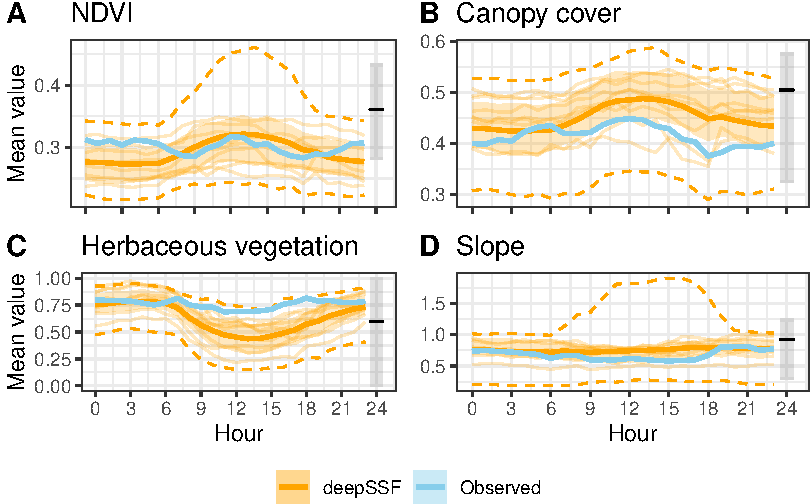
\includegraphics[keepaspectratio]{deepSSF_assessing_trajectories_files/figure-pdf/unnamed-chunk-30-1.pdf}}

\begin{Shaded}
\begin{Highlighting}[]
\FunctionTok{ggsave}\NormalTok{(}\FunctionTok{paste0}\NormalTok{(}\StringTok{"Python/outputs/model\_training/"}\NormalTok{,deepSSF\_dir,}\StringTok{"/hourly\_summaries.png"}\NormalTok{), }\AttributeTok{width=}\DecValTok{180}\NormalTok{, }\AttributeTok{height=}\DecValTok{150}\NormalTok{, }\AttributeTok{units=}\StringTok{"mm"}\NormalTok{, }\AttributeTok{dpi =} \DecValTok{600}\NormalTok{)}
\end{Highlighting}
\end{Shaded}





\end{document}
